\documentclass[twocolumn]{../../common/aa}
%\documentclass[referee]{aa}

\usepackage{graphicx}
\usepackage{amsmath,amsfonts,amssymb}
\usepackage[varg]{txfonts}
\usepackage{color}
\usepackage{natbib}
\usepackage{float}
%\usepackage{stfloats}
\usepackage{dblfloatfix}
\usepackage{afterpage}
\usepackage{ifthen}
\usepackage[morefloats=12]{morefloats}
\usepackage{placeins}
\usepackage{multicol}
\usepackage{multirow}
\bibpunct{(}{)}{;}{a}{}{,}
\usepackage[switch]{lineno}
\definecolor{linkcolor}{rgb}{0.6,0,0}
\definecolor{citecolor}{rgb}{0,0,0.75}
\definecolor{urlcolor}{rgb}{0.12,0.46,0.7}
\usepackage[breaklinks, colorlinks, urlcolor=urlcolor,
    linkcolor=linkcolor,citecolor=citecolor,pdfencoding=auto]{hyperref}
\hypersetup{linktocpage}
\usepackage{bold-extra}
\usepackage{xcolor}
\newcommand{\gray}[0]{\color{gray}}

\usepackage{lipsum}

%\usepackage[grid,
%  gridcolor=red!20,
%  subgridcolor=green!20,
%  gridunit=cm]{eso-pic}


%Planck style file, to be used with A&A style to produce Planck papers for publication.
%
% version 28 September 2010 --- useful macros --- CRL
% version 17 October 2010   --- first cut at important instrument values, from Daniele Mennella and
%                               Francois Bouchet, 13 October 2010 --- CRL
% version 18 October 2010   --- LFI FWHM changed to one value per feed, rather than M & S separately
%                               LFI FWHM uncertainties added for individual feeds.  Corrections made
%                               to LFI values. --- Andrea Zacchei
% version 24 October 2010   --- added to and corrected definitions.  No changes made to instrument
%                               quantities. --- CRL 
% version 31 October 2010   --- added definition of \muKHz. --- CRL
%
% version 15 November 2010  --- fixed conflict with aa.cls in definition of \endtable
%                               by naming the command below "\endPlancktable".  See section
%                               13.16 of the Style Guide.
%
% version 06 December 2010  --- Set up names with and without units.
%                               Add \allearlypapers command to ensure that all early papers are
%                               included in the reference list.
%                               Define macro for the name of the 4He JT cooler.
%
% version 07 December 2010  --- removed extraneous "planck2011-1.2" entry in \allearlypapers
%
% version 12 December 2010  --- added \endPlancktablewide command to set tablenotes to the full
%                               page width in the \begin{table*}...\end{table*} environment when
%                               the ``twocolumn'' option is specified in the \documentclass command.
%                               (It would be more elegant to extract the appropriate width from the
%                               aa.cls system at the time of execution, but that is buried more
%                               deeply in the system than I investigated.)
%
% version 05 January 2011   --- added unit \MJysr.  HFI performance values updated per FRB email
%                               01/05/2011 02:38-0800, and Brendan Crill email 01/05/2011 18:08 -0800.
%
% version 06 January 2011   --- changed \scriptscriptstyle primes to \scriptstyle, to better match the
%                               tx fonts used by A&A.
%
% version 07 January 2011   --- modified \allearlypapers to correspond with final early paper list.  
%                               Fixed 545 GHz center frequency.
%
% version 07 January 2011b  --- changed LFI white-noise sensitivity numbers to correct problem with units
%
% version 05 July 2011      --- added \Msol and \Lsol to get the symbols for solar mass and luminosity.
%                               Deleted previous definitions of \solar and \sol, which were equivalent
%                               to the new \Msol.
%
% version 16 August 2011    --- changed comments on \endPlancktable and \endPlancktablewide for clarity
%
% version 11 September 2011 --- changed definition of \tablenote to make footnote labels italic, as per A\&A
%
% version 26 April 2011     --- changed definition of \Planck to agree with what is said in the Style Guide (!)
%
% version 04 Dec 2013       --- included 2013 results references
%
% version 17 Jan 2014       --- included fix to bibtex file v4.3, i.e. \providecommand{\sorthelp}[1]{}
%
% version 26 Jul 2014       --- fixed incompatibility problem with aa.cls v8.0 and v8.2.  v8.2 should now be used
%                               for all Planck papers.
%                           --- fixed problem in definition of "\all2013resultspapers" that introduced a blanck
%                               into the reference to p06b.
%                           --- removed all the parameter definition stuff at the end.  We weren't using it, and
%                               it took up a lot of space.
%
% version 28 Jan 2015       --- added "\alltwentyfiftennresultspapers" and corrected "\all2013resultspapers" to
%                               "\all20thirteenresultspapers",
%
% Usage:  after the \documentclass[traditabstract]{aa} command in the La\TeX\ input file,
%         add this command:      \input Planck.tex


\def\setsymbol#1#2{\expandafter\def\csname #1\endcsname{#2}}
\def\getsymbol#1{\csname #1\endcsname}

%-----------------------------------------------------------------------
% Planck
%-----------------------------------------------------------------------
\def\Planck{\textit{Planck}}

%-----------------------------------------------------------------------
% The Planck Helium-4 JT cooler
%-----------------------------------------------------------------------
\def\HeJT{$^4$He-JT}

%-----------------------------------------------------------------------
% To include all Planck Early Results papers in the reference lists
%-----------------------------------------------------------------------
\def\allearlypapers{\nocite{planck2011-1.1, planck2011-1.3, planck2011-1.4, planck2011-1.5, planck2011-1.6, planck2011-1.7, planck2011-1.10, planck2011-1.10sup, planck2011-5.1a, planck2011-5.1b, planck2011-5.2a, planck2011-5.2b, planck2011-5.2c, planck2011-6.1, planck2011-6.2, planck2011-6.3a, planck2011-6.4a, planck2011-6.4b, planck2011-6.6, planck2011-7.0, planck2011-7.2, planck2011-7.3, planck2011-7.7a, planck2011-7.7b, planck2011-7.12, planck2011-7.13}}

%-----------------------------------------------------------------------
% To include all Planck 2013 Results papers in the reference lists
%-----------------------------------------------------------------------
\def\alltwentythirteenresultspapers{\nocite{planck2013-p01, planck2013-p02, planck2013-p02a, planck2013-p02d, planck2013-p02b, planck2013-p03, planck2013-p03c, planck2013-p03f, planck2013-p03d, planck2013-p03e, planck2013-p01a, planck2013-p06, planck2013-p03a, planck2013-pip88, planck2013-p08, planck2013-p11, planck2013-p12, planck2013-p13, planck2013-p14, planck2013-p15, planck2013-p05b, planck2013-p17, planck2013-p09, planck2013-p09a, planck2013-p20, planck2013-p19, planck2013-pipaberration, planck2013-p05, planck2013-p05a, planck2013-pip56, planck2013-p06b, planck2013-p01a}}

%-----------------------------------------------------------------------
% To include all Planck 2015 Results papers in the reference lists
%-----------------------------------------------------------------------
\def\alltwentyfifteenresultspapers{\nocite{planck2014-a01, planck2014-a03, planck2014-a04, planck2014-a05, planck2014-a06, planck2014-a07, planck2014-a08, planck2014-a09, planck2014-a11, planck2014-a12, planck2014-a13, planck2014-a14, planck2014-a15, planck2014-a16, planck2014-a17, planck2014-a18, planck2014-a19, planck2014-a20, planck2014-a22, planck2014-a24, planck2014-a26, planck2014-a28, planck2014-a29, planck2014-a30, planck2014-a31, planck2014-a35, planck2014-a36, planck2014-a37, planck2014-ES}}

%-----------------------------------------------------------------------
% Tables
%-----------------------------------------------------------------------
\newbox\tablebox    \newdimen\tablewidth
\def\leaderfil{\leaders\hbox to 5pt{\hss.\hss}\hfil}
%
% use the following definition of \endPlancktable for ApJ style notes to tables, set to the 
%         width of the table
% \def\endPlancktable{\tablewidth=\wd\tablebox 
%
% use the following definitions of \endPlancktable and \endPlancktablewide for A&A style notes 
% set to one-column  or full-page width, respectively
\def\endPlancktable{\tablewidth=\columnwidth 
    $$\hss\copy\tablebox\hss$$
    \vskip-\lastskip\vskip -2pt}
\def\endPlancktablewide{\tablewidth=\textwidth 
    $$\hss\copy\tablebox\hss$$
    \vskip-\lastskip\vskip -2pt}
\def\tablenote#1 #2\par{\begingroup \parindent=0.8em
    \abovedisplayshortskip=0pt\belowdisplayshortskip=0pt
    \noindent
    $$\hss\vbox{\hsize\tablewidth \hangindent=\parindent \hangafter=1 \noindent
    \hbox to \parindent{$^#1$\hss}\strut#2\strut\par}\hss$$
    \endgroup}
\def\doubleline{\vskip 3pt\hrule \vskip 1.5pt \hrule \vskip 5pt}

%-----------------------------------------------------------------------
% useful macros
%-----------------------------------------------------------------------
%
\def\L2{\ifmmode L_2\else $L_2$\fi}
%
\def\dtt{\Delta T/T}
\def\DeltaT{\ifmmode \Delta T\else $\Delta T$\fi}
\def\deltat{\ifmmode \Delta t\else $\Delta t$\fi}
\def\fknee{\ifmmode f_{\rm knee}\else $f_{\rm knee}$\fi}
\def\Fmax{\ifmmode F_{\rm max}\else $F_{\rm max}$\fi}
%
\def\solar{\ifmmode{\rm M}_{\mathord\odot}\else${\rm M}_{\mathord\odot}$\fi}
\def\Msolar{\ifmmode{\rm M}_{\mathord\odot}\else${\rm M}_{\mathord\odot}$\fi}
\def\Lsolar{\ifmmode{\rm L}_{\mathord\odot}\else${\rm L}_{\mathord\odot}$\fi}
%
\def\inv{\ifmmode^{-1}\else$^{-1}$\fi}
\def\mo{\ifmmode^{-1}\else$^{-1}$\fi}
\def\sup#1{\ifmmode ^{\rm #1}\else $^{\rm #1}$\fi}
\def\expo#1{\ifmmode \times 10^{#1}\else $\times 10^{#1}$\fi}
%
\def\,{\thinspace}
\def\lsim{\mathrel{\raise .4ex\hbox{\rlap{$<$}\lower 1.2ex\hbox{$\sim$}}}}
\def\gsim{\mathrel{\raise .4ex\hbox{\rlap{$>$}\lower 1.2ex\hbox{$\sim$}}}}
\let\lea=\lsim
\let\gea=\gsim
\def\simprop{\mathrel{\raise .4ex\hbox{\rlap{$\propto$}\lower 1.2ex\hbox{$\sim$}}}}
%
\def\deg{\ifmmode^\circ\else$^\circ$\fi}
\def\pdeg{\ifmmode $\setbox0=\hbox{$^{\circ}$}\rlap{\hskip.11\wd0 .}$^{\circ}
          \else \setbox0=\hbox{$^{\circ}$}\rlap{\hskip.11\wd0 .}$^{\circ}$\fi}
\def\arcs{\ifmmode {^{\scriptstyle\prime\prime}}
          \else $^{\scriptstyle\prime\prime}$\fi}
\def\arcm{\ifmmode {^{\scriptstyle\prime}}
          \else $^{\scriptstyle\prime}$\fi}
\newdimen\sa  \newdimen\sb
\def\parcs{\sa=.07em \sb=.03em
     \ifmmode \hbox{\rlap{.}}^{\scriptstyle\prime\kern -\sb\prime}\hbox{\kern -\sa}
     \else \rlap{.}$^{\scriptstyle\prime\kern -\sb\prime}$\kern -\sa\fi}
\def\parcm{\sa=.08em \sb=.03em
     \ifmmode \hbox{\rlap{.}\kern\sa}^{\scriptstyle\prime}\hbox{\kern-\sb}
     \else \rlap{.}\kern\sa$^{\scriptstyle\prime}$\kern-\sb\fi}
%
\def\ra[#1 #2 #3.#4]{#1\sup{h}#2\sup{m}#3\sup{s}\llap.#4}
\def\dec[#1 #2 #3.#4]{#1\deg#2\arcm#3\arcs\llap.#4}
\def\deco[#1 #2 #3]{#1\deg#2\arcm#3\arcs}
\def\rra[#1 #2]{#1\sup{h}#2\sup{m}}
%
\def\page{\vfill\eject}
\def\dots{\relax\ifmmode \ldots\else $\ldots$\fi}
%
%-----------------------------------------------------------------------
% units
%-----------------------------------------------------------------------
%
\def\WHzsr{\ifmmode $W\,Hz\mo\,sr\mo$\else W\,Hz\mo\,sr\mo\fi}
\def\mHz{\ifmmode $\,mHz$\else \,mHz\fi}
\def\GHz{\ifmmode $\,GHz$\else \,GHz\fi}
\def\mKs{\ifmmode $\,mK\,s$^{1/2}\else \,mK\,s$^{1/2}$\fi}
\def\muKs{\ifmmode \,\mu$K\,s$^{1/2}\else \,$\mu$K\,s$^{1/2}$\fi}
\def\muKRJs{\ifmmode \,\mu$K$_{\rm RJ}$\,s$^{1/2}\else \,$\mu$K$_{\rm RJ}$\,s$^{1/2}$\fi}
\def\muKHz{\ifmmode \,\mu$K\,Hz$^{-1/2}\else \,$\mu$K\,Hz$^{-1/2}$\fi}
\def\MJysr{\ifmmode \,$MJy\,sr\mo$\else \,MJy\,sr\mo\fi}
\def\MJysrmK{\ifmmode \,$MJy\,sr\mo$\,mK$_{\rm CMB}\mo\else \,MJy\,sr\mo\,mK$_{\rm CMB}\mo$\fi}
\def\microns{\ifmmode \,\mu$m$\else \,$\mu$m\fi}
\def\micron{\microns}
\def\muK{\ifmmode \,\mu$K$\else \,$\mu$\hbox{K}\fi}
\def\microK{\ifmmode \,\mu$K$\else \,$\mu$\hbox{K}\fi}
\def\muW{\ifmmode \,\mu$W$\else \,$\mu$\hbox{W}\fi}
\def\kms{\ifmmode $\,km\,s$^{-1}\else \,km\,s$^{-1}$\fi}
\def\kmsMpc{\ifmmode $\,\kms\,Mpc\mo$\else \,\kms\,Mpc\mo\fi}
%
%
%----------------------------------------------------------------------
% set up machinery to list Planck papers in roman numeral order.
%----------------------------------------------------------------------

\providecommand{\sorthelp}[1]{}


\def\WMAP{\emph{WMAP}}
\def\WMAPnine{\emph{WMAP9}}
\def\COBE{\emph{COBE}}
\def\wmap{\emph{WMAP}}
\def\planck{\emph{Planck}}
\def\Planck{\emph{Planck}}
\def\LCDM{$\Lambda$CDM}
\def\ffp{FFP6}
\def\unionmask{U73}
\def\nside{N_{\mathrm{side}}}

\def\healpix{\texttt{HEALPix}}
\def\commander{\texttt{Commander}}
\def\commanderone{\texttt{Commander1}}
\def\commandertwo{\texttt{Commander2}}
\def\commanderthree{\texttt{Commander3}}
\def\ruler{\texttt{Ruler}}
\def\comrul{\texttt{Commander-Ruler}}
\def\CR{\texttt{C-R}}
\def\nilc{\texttt{NILC}}
\def\gnilc{\texttt{GNILC}}
\def\sevem{\texttt{SEVEM}}
\def\smica{\texttt{SMICA}}
\def\CamSpec{\texttt{CamSpec}}
\def\Plik{\texttt{Plik}}
\def\XFaster{\texttt{XFaster}}
\def\sroll2{\texttt{SRoll2}}

\newcommand{\phm}{\phantom{-}}
\newcommand{\dv}[0]{\vec{d}}
\renewcommand{\t}[0]{\vec{t}}
\newcommand{\A}[0]{\mathrm{A}}
\newcommand{\B}[0]{\mathrm{B}}
\newcommand{\Y}[0]{\tens{Y}}
\newcommand{\n}[0]{\vec{n}}
\newcommand{\red}[0]{\color{red}}
\newcommand{\green}[0]{\color{green}}
\newcommand{\s}[0]{\vec{s}}
\renewcommand{\a}[0]{\vec{a}}
\newcommand{\m}[0]{\vec{m}}
\newcommand{\bv}[0]{\vec{b}}
\newcommand{\f}[0]{\vec{f}}
\newcommand{\F}[0]{\tens{F}}
\newcommand{\T}[0]{\tens{T}}
\newcommand{\Cp}[0]{\tens{C}}
\renewcommand{\L}[0]{\tens{L}}
\newcommand{\g}[0]{\vec{g}}
\newcommand{\N}[0]{\tens{N}}
\newcommand{\M}[0]{\tens{M}}
\newcommand{\iN}[0]{\tens{N}^{-1}}
\newcommand{\iM}[0]{\tens{M}^{-1}}
\newcommand{\w}[0]{\vec{w}}
\renewcommand{\S}[0]{\tens{S}}
\renewcommand{\r}[0]{\vec{r}}
\renewcommand{\u}[0]{\vec{u}}
\newcommand{\q}[0]{\vec{q}}
\renewcommand{\v}[0]{\vec{v}}
\renewcommand{\P}[0]{\tens{P}}
\newcommand{\dt}[0]{d_t}
\newcommand{\di}[0]{d_i}
\newcommand{\nt}[0]{n_t}
\newcommand{\st}[0]{s_t}
\newcommand{\mt}[0]{m_t}
\newcommand{\ft}[0]{f_t}
\newcommand{\Te}[0]{T_{\rm e}}
\newcommand{\EM}[0]{\rm EM}
\newcommand{\mathsc}[1]{{\normalfont\textsc{#1}}}
\newcommand{\hi}{\ensuremath{\mathsc {Hi}}}
\newcommand{\bpbold}{\bfseries{\scshape{BeyondPlanck}}}
\newcommand{\BP}{\textsc{BeyondPlanck}}
\newcommand{\bp}{\textsc{BeyondPlanck}}
\newcommand{\cosmoglobe}{\textsc{Cosmoglobe}}
\newcommand{\Cosmoglobe}{\textsc{Cosmoglobe}}
\newcommand{\lfi}[0]{LFI}
\newcommand{\hfi}[0]{HFI}
\newcommand{\npipe}[0]{\texttt{NPIPE}}
\newcommand{\K}[0]{\textsl K}
\newcommand{\Ka}[0]{\textsl{Ka}}
\newcommand{\Q}[0]{\textsl Q}
\newcommand{\V}[0]{\textsl V}
\newcommand{\W}[0]{\textsl W}
\newcommand{\e}{\mathrm e}
\newcommand{\cvar}{\ensuremath{c(\vartheta, \varphi, \psi)}}


\def\Tcmb{\ifmmode T_\mathrm{CMB}\else $T_{\mathrm{CMB}}$\fi}
\def\Tdust{\ifmmode T_\mathrm{d}\else $T_{\mathrm{d}}$\fi}
\def\scmb{\ifmmode s_\mathrm{CMB}\else $s_{\mathrm{CMB}}$\fi}
\def\squad{\ifmmode s_\mathrm{quad}\else $s_{\mathrm{quad}}$\fi}
\def\ssynch{\ifmmode s_\mathrm{s}\else $s_\mathrm{s}$\fi}
\def\sdust{\ifmmode s_\mathrm{d}\else $s_{\mathrm{d}}$\fi}
\def\ssdust{\ifmmode s_\mathrm{sd}\else $s_{\mathrm{sd}}$\fi}
\def\same{\ifmmode s_\mathrm{ame}\else $s_{\mathrm{ame}}$\fi}
\def\ssrc{\ifmmode s_\mathrm{src}\else $s_{\mathrm{src}}$\fi}
\def\sco{\ifmmode s_\mathrm{CO}\else $s_{\mathrm{CO}}$\fi}
\def\sff{\ifmmode s_\mathrm{ff}\else $s_{\mathrm{ff}}$\fi}
\def\gff{\ifmmode g_\mathrm{ff}\else $g_{\mathrm{ff}}$\fi}
\def\fsynch{\ifmmode f_\mathrm{s}\else $f_{\mathrm{s}}$\fi}
\def\fsd{\ifmmode f_\mathrm{sd}\else $f_{\mathrm{sd}}$\fi}
\def\fame{\ifmmode f_\mathrm{ame}\else $f_{\mathrm{ame}}$\fi}
\def\alphasrc{\ifmmode \alpha_\mathrm{src}\else $\alpha_{\mathrm{src}}$\fi}
\def\bdust{\ifmmode \beta_\mathrm{d}\else $\beta_{\mathrm{d}}$\fi}
\def\bsynch{\ifmmode \beta_\mathrm{s}\else $\beta_{\mathrm{s}}$\fi} 
\def\bsun{\ifmmode \beta_\mathrm{sun}\else $\beta_{\mathrm{sun}}$\fi} 
\def\nuzeros{\ifmmode \nu_{0,\mathrm{s}}\else $\nu_{0,\mathrm{s}}$\fi} 
\def\nuzeroff{\ifmmode \nu_{0,\mathrm{ff}}\else $\nu_{0,\mathrm{ff}}$\fi} 
\def\nuzerod{\ifmmode \nu_{0,\mathrm{d}}\else $\nu_{0,\mathrm{d}}$\fi} 
\def\nuzeroame{\ifmmode \nu_{0,\mathrm{ame}}\else $\nu_{0,\mathrm{ame}}$\fi} 
\def\nuzerosd{\ifmmode \nu_{0,\mathrm{}}\else $\nu_{0,\mathrm{sd}}$\fi} 
\def\nuzerosrc{\ifmmode \nu_{0,\mathrm{src}}\else $\nu_{0,\mathrm{src}}$\fi} 
\def\nup{\ifmmode \nu_{\mathrm{p}}\else $\nu_{\mathrm{p}}$\fi} 
\def\alphasd{\ifmmode \alpha_{\mathrm{sd}}\else $\alpha_{\mathrm{sd}}$\fi} 
\def\Te{\ifmmode T_{\mathrm{e}}\else $T_{\mathrm{e}}$\fi} 
\def\kB{\ifmmode k_\mathrm{B}\else $k_{\mathrm{B}}$\fi} 



\usepackage[T1]{fontenc}


\def\bC{\tens{C}}
\def\ba{\vec{a}}
\def\ncha{N_\mathrm{cha}}
\def\nfg{N_\mathrm{fg}}

\newcommand{\ncorr}{\vec n_\mathrm{corr}}
\newcommand{\data}{\vec d}
\newcommand{\Dbp}{\Delta_\mathrm{bp}}

%\modulolinenumbers[5]
%\linenumbers

\newcommand{\includegraphicsdpi}[3]{
    \pdfimageresolution=#1  % Change the dpi of images
    \includegraphics[#2]{#3}
    \pdfimageresolution=72  % Change it back to the default
}

\renewcommand{\topfraction}{1.0}	% max fraction of floats at top
    \renewcommand{\bottomfraction}{1.0}	% max fraction of floats at bottom
    %   Parameters for TEXT pages (not float pages):
    \setcounter{topnumber}{2}
    \setcounter{bottomnumber}{2}
    \setcounter{totalnumber}{4}     % 2 may work better
    \setcounter{dbltopnumber}{2}    % for 2-column pages
    \renewcommand{\dbltopfraction}{0.9}	% fit big float above 2-col. text
    \renewcommand{\textfraction}{0.04}	% allow minimal text w. figs
    %   Parameters for FLOAT pages (not text pages):
    \renewcommand{\floatpagefraction}{0.9}	% require fuller float pages
	% N.B.: floatpagefraction MUST be less than topfraction !!
    \renewcommand{\dblfloatpagefraction}{0.9}	% require fuller float pages

\def\adj{^{\dagger}}
\def\tp{^{\rm T}}
\def\inv{^{-1}}
\def\lm{{\ell m}}

\begin{document}

\title{\bfseries{\Cosmoglobe\ DR 1. I. Improved \emph{Wilkinson Microwave Anisotropy Probe} frequency maps by Bayesian end-to-end analysis}}
%This author list corresponds to \title{Author list for L04\_CMB\_Foregrounds\_Extraction}
%Prepared by M. Lopez-Caniego (Marcos.Lopez.Caniego@sciops.esa.int), ESAC/ESA
%This version is from Thu Jul 12 18:11:48 2018 CET
%\subtitle{There are 152 co-authors in this list}
\newcommand{\oslo}[0]{1}
\newcommand{\iiabangalore}[0]{2}

\author{\small
D.~J.~Watts\inst{\ref{uio}}\thanks{Corresponding author: D.~J.~Watts; \url{duncanwa@astro.uio.no}}
\and
A.~Basyrov\inst{\ref{uio}}
\and
H.~T.~Ihle\inst{\ref{uio}}
\and
S.~Paradiso\inst{\ref{waterloo}}
\and
F.~Rahman\inst{\ref{iiabangalore}}
\and
H.~Thommesen\inst{\ref{uio}}
\and
M.~Bersanelli\inst{\ref{milan}}
\and
L.~A.~Bianchi\inst{\ref{milan}}
\and
M.~Brilenkov\inst{\ref{uio}}
\and
L.~P.~L.~Colombo\inst{\ref{milan}}
\and
H.~K.~Eriksen\inst{\ref{uio}}
\and
J.~R.~Eskilt\inst{\ref{uio},\ref{imperial}}
\and
K.~S.~F.~Fornazier\inst{\ref{saopaulo}}
\and
C.~Franceschet\inst{\ref{milan}}
\and
U.~Fuskeland\inst{\ref{uio}}
\and
M.~Galloway\inst{\ref{uio}}
\and
E.~Gjerl\o w\inst{\ref{uio}}
\and
B.~Hensley\inst{\ref{princeton}}
\and
L.~T.~Hergt\inst{\ref{ubc}}
\and
D.~Herman\inst{\ref{uio}}
\and
G.~A.~Hoerning\inst{\ref{saopaulo}}
\and
K.~Lee\inst{\ref{uio}}
\and
J.~G.~S.~Lunde\inst{\ref{uio}}
\and
A.~Marins\inst{\ref{saopaulo},\ref{ustofc}}
\and
S.~K.~Nerval\inst{\ref{dunlap1},\ref{dunlap2}}
\and
S.~K.~Patel\inst{\ref{iit_bhu}}
\and
M.~Regnier\inst{\ref{apc}}
\and
M.~San\inst{\ref{uio}}
\and
S.~Sanyal\inst{\ref{iit_bhu}}
\and
N.-O.~Stutzer\inst{\ref{uio}}
\and
A.~Verma\inst{\ref{iit_bhu}}
\and
I.~K.~Wehus\inst{\ref{uio}}
\and
Y.~Zhou\inst{\ref{berkeley}}
}
\institute{\small
Institute of Theoretical Astrophysics, University of Oslo, Blindern, Oslo, Norway\label{uio}
\and
Waterloo Centre for Astrophysics, University of Waterloo, Waterloo, ON N2L 3G1, Canada\label{waterloo}
\and
Indian Institute of Astrophysics, Koramangala II Block, Bangalore, 560034, India\label{iiabangalore}
\and
Dipartimento di Fisica, Università degli Studi di Milano, Via Celoria, 16, Milano, Italy\label{milan}
\and
Imperial Centre for Inference and Cosmology, Department of Physics, Imperial College London, Blackett Laboratory, Prince Consort Road, London SW7 2AZ, United Kingdom\label{imperial}
\and
Instituto de Física, Universidade de São Paulo - C.P. 66318, CEP: 05315-970, São Paulo, Brazil\label{saopaulo}
\and
Department of Astrophysical Sciences, Princeton University, 4 Ivy Lane, Princeton, NJ 08540\label{princeton}
\and
Department of Physics and Astronomy, University of British Columbia, 6224 Agricultural Road, Vancouver BC, V6T1Z1, Canada\label{ubc}
\and
Department of Astronomy,  University of Science and Technology of China, Hefei, China\label{ustofc}
\and
David A. Dunlap Department of Astronomy \& Astrophysics, University of Toronto, 50 St. George Street, Toronto, ON M5S 3H4, Canada\label{dunlap1}
\and
Dunlap Institute for Astronomy \& Astrophysics, University of Toronto, 50 St. George Street, Toronto, ON M5S 3H4, Canada\label{dunlap2}
\and
Department of Physics, Indian Institute of Technology (BHU), Varanasi - 221005, India\label{iit_bhu}
\and
Laboratoire Astroparticule et Cosmologie (APC), Université Paris-Cité, Paris, France\label{apc}
\and
Department of Physics, UC Berkeley\label{berkeley}
}

 %\author{V.~Arsenijevic\inst{\ref{inst1}}\and S.~Fabbro\inst{\ref{inst2}}\and
%A.~M.~Mour\~ao\inst{\ref{inst3}}\and A.~J.~Rica da Silva\inst{\ref{inst1}}}
%
%\institute{Multidisciplinar de Astrof\'{\i}sica, IST, Avenida Rovisco Pais, 1049
%Lisbon, Portugal\email{...}\label{inst1} \and < Multidisciplinar de Astrof\'{\i}sica, IST, Avenida Rovisco Pais, 1049 Lisbon, Portugal\email{...}\label{inst2}
%\and
%Multidisciplinar de Astrof\'{\i}sica, IST, Avenida Rovisco Pais, 1049
%Lisbon, Portugal\email{...}\label{inst3}
%} 

%\authorrunning{From BeyondPlanck to Cosmoglobe}
\authorrunning{Watts et al.}
\titlerunning{\cosmoglobe\ \wmap{}  analysis}

\abstract{
  We present the first joint analysis of \textit{WMAP} and \textit{Planck} LFI time-ordered data, processed within the Bayesian end-to-end \commander\ framework. This framework builds directly on a similar analysis of the LFI measurements by the \BP\ collaboration, and approaches the CMB analysis challenge through Gibbs sampling of a global posterior distribution. The computational cost of producing one complete \WMAP+LFI Gibbs sample is 581\,CPU-hr, including calibration, mapmaking, and component separation, of which 389\,CPU-hr is spent on \WMAP\ low-level processing; this demonstrates that end-to-end Bayesian analysis of the \WMAP\ data is computationally feasible. We find that our \WMAP\ posterior mean temperature sky maps are largely consistent with the official maps, and the resulting CMB power spectrum is in excellent agreement with previous results. The most notable difference is a slightly lower CMB quadrupole amplitude of $\sigma_2 = 120\pm65\muK^2$, as compared to $\sigma_2 = 229\pm97\muK^2$ in the \BP\ analysis. In contrast, our \WMAP\ polarization maps differ more notably from the official results, and in general they exhibit  lower large-scale residuals, most likely attributable to a better constrained gain and transmission imbalance model; it is particularly noteworthy that our \W-band sky maps appear statistically consistent with the \V-band maps. For the first time, \WMAP-minus-LFI frequency map differences appear visually consistent with instrumental noise over most of the sky. Still, we identify three specific issues that require additional work, namely 1) low-level noise modeling, 2) quadrupole residuals in the $V$- and $W$-band temperature maps at the 2\muK\ level; and 3) a strong degeneracy between the absolute $K$-band calibration and the dipole of the anomalous microwave emission component. Nevertheless, we believe that the reprocessed \WMAP\ maps presented here are significantly cleaner in terms of systematic uncertainties than the official \WMAP\ maps. Both sky maps and the associated code are made publicly available through the \cosmoglobe\ web page. 
}

\keywords{ISM: general -- Cosmology: observations, polarization,
    cosmic microwave background, diffuse radiation -- Galaxy:
    general}

\maketitle

%\hypersetup{linkcolor=black}
\tableofcontents
%\hypersetup{linkcolor=red} 




\section{Introduction}
\label{sec:introduction}

%\textbf{Describe WMAP highlights, establishment of firm LCDM model. Brief summary of Planck, Commander, BeyondPlanck, and then Cosmoglobe; WMAP is first major extension of the end-to-end framework, and marks the transition from classical single-experiment TOD analysis to multi-experiment TOD analysis. A brave new world.}

The discovery of the cosmic microwave background (CMB) by \citet{penzias:1965} marked a paradigm shift in the field of cosmology, providing direct evidence that the Universe was once much hotter than it is today, effectively ruling out the steady-state theory of the universe \citep{dicke:1965}. This discovery spurred a series of ground-breaking cosmological experiments, including the Nobel Prize-winning measurements by \COBE-FIRAS that confirmed the blackbody nature of the CMB \citep{mather:1994} and \COBE-DMR that measured temperature variations from the primordial gravitational field \citep{smoot:1992}.

The NASA-funded \textit{Wilkinson Microwave Anisotropy Probe} (\WMAP; \citealp{bennett2003:MAP}) mission was launched a decade after \COBE-DMR, and mapped the microwave sky with 45 times higher sensitivity and 33 times higher angular resolution, and thereby revolutionizing our understanding of early universe physics \citep{bennett2003:MAP}. As quantified by \citet{bennett2012}, the permissable parameter space volume for a standard $\Lambda$CDM model was decreased by a factor of 68,000 by \WMAP, and the best pre-\WMAP\ determination of the age of the universe was $t_0<14\,\mathrm{Gyr}$ from Boomerang \citep{lange:2001}, with best-fit values of 9--11\,Gyr; the latter values in apparent contradiction with direct measurements of the oldest globular clusters \citep{hu:2001}.

The ESA-led \Planck\ satellite \citep{planck2016-l01} was developed concurrently with \WMAP, and their operation lifetimes briefly overlapped, with \Planck\ observing from 2009--2013 and \WMAP\ from 2001--2011. \Planck's stated goal was to fully characterize the primary CMB temperature fluctuations from recombination, as well as to characterize the polarized microwave sky on large angular scales.  Overall, \Planck's raw CMB sensitivity was an order of magnitude higher than \WMAP's, and its angular resolution three times higher. Today, \Planck\ represents the state-of-the-art in terms of full-sky microwave sky measurements.

\Planck\ comprised two independent experiments, namely the Low Frequency Instrument (LFI; \citealp{planck2016-l02}) and High Frequency Instrument (HFI; \citealp{planck2016-l03}), respectively. The LFI detectors were based on HEMT (high electron mobility transistor) amplifiers, spanning three frequency channels between 30 and 70\,GHz, while the HFI detectors were based on TES (transition edge sensitive) bolometers, and spanned six frequency channels between 100 and 857\,GHz. For comparison, \WMAP\ was also HEMT-based, with comparable sensitivity to LFI alone, and spanned five frequencies between 23 and 94\,GHz. At the same time, the two experiments implemented very different scanning strategies, and as a result they are highly complementary and synergistic; together they provide a clearer view of the low-frequency microwave sky than either can alone.

%As opposed to \WMAP, which used minimal \COBE\ data in its fiducial analysis, \Planck's initial release calibrated off of \WMAP's Solar dipole solution, and the Galactic component separation solution found in  \citet{planck2014-a12} by \commander\ \citep{jewell2004,eriksen:2004,eriksen2006,eriksen2008} made use of \WMAP\ frequency maps. Most crucially, the \Planck\ and \WMAP\ maps are of similar quality that meaningful comparisons can be made between them. This last aspect has been critical, especially for the \Planck\ Low Frequency Instrument (LFI), whose channels lie between those of \WMAP.

Towards the end of the \Planck\ analysis phase it became clear that the interplay between instrument calibration and astrophysical component separation represented a main limiting factor in terms of systematic effects for high signal-to-noise measurements \citep{planck2016-l02}. Specifically, in order to calibrate the instrument to sufficient precision, it became clear that it was necessary to know the true sky to a comparably high precision -- but to know the sky, it was also necessary to know the instrumental calibration. The data analysis is thus fundamentally circular and global in nature. The final official \Planck\ LFI analysis performed four complete iterations between calibration and component separation \citep{planck2016-l02}, aiming to probe this degeneracy. However, it was clearly recognized that this was not sufficient to reach full convergence, and this sub-optimality led to the \BP\ project \citep{bp01}, which aimed to perform thousands of complete analysis cycles, as opposed to just a handful. This framework was implemented using the \commanderthree\ \citep{bp03} code, a CMB Gibbs sampler that performs integrated high-level and low-level parameter estimation in a single integrated framework. This analysis demonstrated the feasibility of a full end-to-end Gibbs sampling analysis in the CMB framework, while providing the highest-quality LFI maps to date.

Rather than simply probing the degeneracy between instrument calibration and component separation, a better solution is to actually break it. The optimal approach to do so is by jointly analyzing complementary datasets, each of which provide key information regarding the full system. This insight led to the \cosmoglobe\footnote{\url{https://cosmoglobe.uio.no}} initiative, which is an Open Source and community-wide effort that aims to derive a single joint model of the radio, microwave, and sub-millimeter sky by combining all available state-of-the-art experiments. An obvious first extension of the LFI-oriented \BP\ project is to analyze the \WMAP\ measurements in the same framework. Indeed, already as part of the \BP\ suite of papers, \citet{bp17} integrated \WMAP\ \Q-band time-ordered data (TOD) into the \commanderthree\ framework, calibrated off of the \BP\ sky model.
%Beyond demonstrating that \commanderthree\ can be applied to non-\Planck\ data, this analysis uncovered an instrumental effect not previously described in the literature, namely a spurious polarization signal induced by the coupling of the Solar dipole, sidelobes, and horn transmission imbalance. 

In this paper, we present the first end-to-end Bayesian analysis of the full \WMAP\ TOD, processed within the \commander\ framework, and this constitutes the first \cosmoglobe\ Data Release (DR1). In doing so, this paper in fact also presents the first ever joint analysis of two major CMB experiments (LFI and \WMAP) at the lowest possible level, and it therefore constitutes a major milestone of the \cosmoglobe\ initiative. In the future, many more datasets will be added, gradually providing stronger and stronger constraints on the true astrophysical sky. Each new experiment will then also in turn improve the instrumental calibration of all previous experiments. 

The rest of this paper is organized as follows. In Sect.~\ref{sec:methods}, we provide a brief review of the Bayesian end-to-end statistical framework used in this work, before describing the underlying data and computational expenses in Sect.~\ref{sec:data}. The main results, as defined by the global posterior distribution, are described in Sects.~\ref{sec:instrument}--\ref{sec:astrophysics}, summarizing instrumental parameters, frequency sky maps, and astrophysical results, respectively. In Sect.~\ref{sec:systematics} we quantify the systematic error budget for this analysis, while we address a few minor unresolved issues in Sect.~\ref{sec:issues} that should be addressed in future work. We conclude in Sect.~\ref{sec:conclusions}, and lay a path forward for the \cosmoglobe\ project.


% A to-do list:
% 
% \begin{itemize}
%	\item Find the time it takes for each beam to cross itself.
%	\item Fix AME model (\textit{I'm not sure what motivated this, perhaps not necessary?}
%	\item Fix noise model (\textit{Explained because of the Bessel filter plus linear trend})
% \end{itemize}
% 
% A table to include
% \begin{itemize}
%	\item Spin rate -- 0.464\,rpm (7.57 mHz), but translations to $2.6$ degrees per second in boresight?
%	\item Precession -- 1 rev/hour (0.3 mHz)
%	\item Signal bandwidth extends from 0.008--8 Hz \citep{jarosik2003a}
%	\item Beam size in degrees -- 0.88, 0.66, 0.51, 0.35, 0.22.
% \end{itemize}


%The cosmic microwave background (CMB) is the most direct probe of the initial state of the Universe. Since the initial discovery of the CMB \citep{penzias:1965}, subsequent experiments have continually refined the measurements, to the extent that the \WMAP\ results are generally considered bringing cosmology into the regime of precision science \citep{bennett2012}. Prior to \WMAP, it was common for CMB experiments to be superseded by more sensitive successors, with the noteworthy exceptions of \COBE/FIRAS and \COBE/DIRBE.
%
%The \planck\ experiment, rather than superseding \WMAP, consistently used \WMAP\ data in its calibration, component separation, and cosmological analyses. The most direct comparison between \WMAP\ and \Planck\ is through analysis of the two experiments' frequency maps, as \WMAP's \K, \Ka, \Q, \V, and \W\ maps are interleaved by the \Planck\ LFI's 30, 44, and 70\,GHz bands. Since the initial \Planck\ data release, there have been several analyses comparing the two experiments by members of the \WMAP\ team \citep{larson2014,addison:2016,huang:2018,weiland:2018,weiland:2022} and by the \Planck\ team \citep{planck2014-a13,planck2016-l06,planck2016-l05}.
%
%While the \WMAP\ low-level analysis has remained stable since \citet{bennett2012}, there has been continued work on \Planck\ time-ordered data processing, notably \bp\ for the LFI instrument \citep{bp01}, \sroll2\ for the HFI instrument \citep{delouis:2019}, and \Planck\ DR4 for both LFI and HFI \citep[\npipe,][]{npipe}. The LFI instrument in particular has had several systematics mitigated by improved analysis, particularly a smoothed gain solution and an improved noise model \citep{npipe,bp06,bp07,bp10}. When comparing \WMAP\ \K-band with the \Planck\ LFI data, the residuals are mainly characterized by \WMAP's poorly measured modes, which can be seen clearly in Figures 50 and 51 of \citet{npipe} and Figures 4 and 7 of \citet{bp14}.
%
%One of the primary outcomes of the \BP\ project is that end-to-end analysis of a dataset with poorly measured modes can be mitigated by a joint analysis with another dataset that measures these modes well. In particular, \Planck\ LFI had large scale polarizated modes aligned with the instrument's scan strategy, induced by relative errors between different polarization-sensitive radiometers \citep{bp07}. The \bp\ project mitigated this by using \WMAP's polarized \Ka--\V\ maps for component separation, where these modes were well-measured. In order to properly combine these datasets, the polarized maps were the $N_\mathrm{side}=16$ \healpix\footnote{\url{http://healpix.sourceforge.net} \citep{gorski2005}} products with a pixel-pixel covariance matrix that explicitly projected out the poorly measured modes.
%
%In principle, the \Planck\ experiment can be used to identify \WMAP's poorly measured modes in the same way that \WMAP\ removed \Planck's poorly measured modes. This was shown in \citet{bp17}, in which \WMAP\ data was calibrated against the \bp\ sky model, and the resulting maps differed from the \WMAPnine\ products mainly through the lack of the poorly measured modes. This work mainly functioned as a demonstration that the \commanderthree\ framework could be applied to the \WMAP\ dataset, and was not a true end-to-end analysis.
%
%In this work, we present the first joint TOD analysis in the \cosmoglobe\footnote{\url{cosmoglobe.uio.no}} framework, in which we analyze the full \WMAP\ dataset along with time-ordered \Planck\ LFI data. In Sect.~\ref{sec:methods}, we review the \cosmoglobe\ statistical framework and the data processing for \Planck\ LFI and \WMAP\ in the \commanderthree\ pipeline. In Sect.~\ref{sec:freqmaps}, we present the \Planck\ and \WMAP\ joint frequency maps, and compare these frequency maps with the fiducial analyses in Sect.~\ref{sec:comparison}. We discuss outstanding systematic errors and the propagation of uncertainty in Sect.~\ref{sec:systematics}. We summarize our results and lay a path forward in Sect.~\ref{sec:conclusions}.


\section{End-to-end Bayesian CMB analysis}
\label{sec:methods}

The general computational analysis framework used in this work has been described in detail by \citet{bp01} and \citet{bp17} and references therein. In this section, we give a brief summary of the main points, and emphasize in particular the differences with respect to earlier work. 
%In particular, Sect.~\ref{sec:lfi_bp} gives an overview of the \bp\ project's reanalysis of \Planck\ LFI data, Sect.~\ref{sec:official_pipeline} provides a brief overview of the official \WMAP\ pipeline, and Sect.~\ref{sec:wmap_instmodel} details the data model that is used in the current LFI+\WMAP\ end-to-end Gibbs sampling analysis.

\subsection{LFI and \bp}
\label{sec:lfi_bp}

The \bp\ project \citep{bp01} was the first true application of end-to-end Gibbs sampling in the framework of CMB data analysis. The \Planck\ LFI data had been gradually improved through each \Planck\ data release, specifically  PR1 \citep{planck2014-a03}, PR2 \citep{planck2014-a03}, PR3 \citep{planck2016-l02}, and PR4 \citep{planck2014-a03}. Even after PR4, however, the final LFI maps still failed significant polarization null tests (in particular for the 44\,GHz frequency channel), in particular due to contained poorly measured realtive gain uncertainty modes. Indeed, already the PR3 analysis noted a strong degeneracy between the LFI gain solution and the astrophysical foreground model, and to break these the \Planck\ LFI Data Processing Center (DPC) implemented an iterative scheme in which the various low-level processing and component separation operations were performed sequentially and repeatedly. However, because these iterations were performed manually with significant amounts of human interactions, these scheme was very slow, and only four full cycles were completed before the \Planck\ collaboration ended. A main motivation for the \BP\ project was to automate this process, and perform thousands of such iterations, rather than just four. 

This work was highly successful, and the \bp\ collaboration was able to generate the first LFI maps with true joint estimation of sky components and underlying instrumental parameters through a statistical process called Gibbs sampling \citep{bp01,bp03,bp10}. The code used for this process was called \commanderthree\ \citep{bp03}. The resulting Gibbs chains allowed for data-driven estimates of the instrumental properties to be determined by exploring the degeneracies between the low-level instrumental parameters themselves and our knowledge of the sky \citep{bp13,bp14}, and in doing so resulted in new state-of-the-art and low-systematics LFI maps.

\subsection{Official \WMAP\ instrument model and analysis pipeline}
\label{sec:official_pipeline}

The main goal of the current paper is to perform a similar analysis with the \WMAP\ time-ordered data, and thereby solve some of the long-standing unresolved issues with the official maps, in particular related to poorly constrained large-scale polarization modes. Before presenting our algorithm, however, it is useful for reference purposes to briefly review the official \WMAP\ instrument model and analysis pipeline, which improved gradually over a total of five data releases, often referred to as the 1-, 3-, 5-, 7, and 9-year data releases, respectively. Unless otherwise noted, we will refer to the final 9-year results in the following. The official \WMAP\ results delivered by \citet{bennett2012} will be referred to by \WMAPnine.

The \WMAP\ satellite carried forty differential polarization-sensitive radiometers grouped as differencing assemblies (DAs), where one pair was sensitive to the difference in signal at one polarization orientation and the other pair sensitive to the orthogonal polarization. In total, there were ten DAs, which were distributed as one \K-band (23\,GHz), one \Ka-band (33\,GHz), two \Q-band (41\,GHz), two \V-band (61\,GHz), and four \W-band (94\,GHz) DAs.  Each DA is labelled, \textsl{Xn}, where \textsl{X} is the band label and \textsl{n} is index of the DA in question, e.g., \K1 or \W3. A second digit \textsl{m} is used to denote whether which linear polarization, ``1'' or ``2'', the radiometer is sensitive to. Additionally, each detector is a two-channel device that is internally left or right ``jammed'' with a $180^\circ$ phase lag in the electronics \citep{jarosik2003:MAP}. These datastreams are further labeled by an integer \textsl{k} that takes values ``3'' or ``4'' \citep{hinshaw2003a}. For example, the label \Q223 refers to the second \Q-band DA with corresponding to the second polarization orientation's first channel.

The \WMAP\ bandpasses were measured pre-launch on ground, sweeping a signal source through 201 frequencies and recording the output \citep{jarosik2003:MAP}. The bandpass responses have not been updated since the initial data release. However, as noted in \citet{bennett2012}, there has been an observed drift in the center frequency of \K, \Ka, \Q, and \V-band corresponding to a $\sim$$\,0.1\,\%$ decrease over time. In practice, this did not affect the \WMAP\ data processing because each year was mapped separately and co-added afterwards. An effective frequency calculator was delivered in the DR5 release as part of the IDL library to mitigate this effect during astrophysical analyses.\footnote{\url{https://lambda.gsfc.nasa.gov/product/wmap/dr5/m_sw.html}}

The beams were characterized in the form of maps, with separate products for the near-field and far-field. The main beam and near sidelobes were characterized using a combination of physical optics codes and observations of Jupiter for each horn separately. The maps of Jupiter were then combined with the best-fit physical optics codes to create a map of the beam response \citep{hill2009,weiland2010,bennett2012}.
Far sidelobes were estimated using a combination of laboratory measurements and Moon data taken during the mission \citep{barnes2003}, as well as a physical optics model described by \citet{hinshaw2009}. To remove the far sidelobe  in the TOD, an estimate was calculated by convolving the intensity map and the orbital dipole signal with the measured sidelobe signal \citep{jarosik2007}. Although the sidelobe pickup was modeled by \citet{barnes2003}, it was determined that the results were small enough to be neglected and have not been explicitly reported in any of the subsequent \WMAP\ data releases.

The \WMAP\ pointing solution was determined using the boresight vectors of individual feedhorns in spacecraft coordinates, in combination with on-board star trackers. Thermal flexure of the tracking structure introduced small pointing errors, as discussed by \citet{jarosik2007}. Using the temperature variation measured by housekeeping data, the quaternion pointing solution was corrected using a linear model that depends on arcsecond per kelvin. The residual pointing errors were computed using observations of Jupiter and Saturn, and the reported upper limit was given as 10\arcsec\ \citep{bennett2012,wmapexsupp}.

The \WMAP\ data were calibrated by jointly estimating the time-dependent gains, $\g$, and baselines, $\bv$, as described by \citet{hinshaw2007}, \citet{hinshaw2009}, and \citet{jarosik2010}.
The TOD were intially modeled as having
constant gain and baseline for a 1--24\,hour period, with parameters that were fit to the orbital
dipole assuming $T_0$ from \citet{mather:1999} and a map made from a previous
iteration of the mapmaking procedure. Once the gain and baseline solution had
converged, the data were fit to a parametric form of the radiometer response
as a function of housekeeping data, given in Appendix~A of \citet{wmapexsupp}.

One unique feature of the \WMAP\ instrument is that it includes differential pointing. That is, \WMAP\ had two primary mirrors positioned on opposite sides of the vertical satellite axis, tilted approximately $19.5^\circ$ downwards. In total, when horn A was pointed at pixel $p_\A$, horn B was pointed at a pixel $p_\B$ approximately $141^\circ$ away \citep{page2003:MAP}. The incoming radiation was differenced in the electronics before being deposited on the detectors, essentially recording radiation proportional to $\boldsymbol m_\A-\boldsymbol m_\B$ and $\boldsymbol m_\B-\boldsymbol m_\A$ \citep{jarosik2003:MAP}. Each pair of radiometers had a partner pair of radiometers that observed the same pixels with sensitivity to the orthogonal polarization direction. Taking these effects all into account, the total data model for a single radiometer is given by
\begin{align}
	d_t^\mathrm{imbal}&\propto (1+x_\mathrm{im})T_{p_\A}-(1-x_\mathrm{im})T_{p_\B}
	\\
	&=(T_{p_\A}-T_{p_\B})+x_\mathrm{im}(T_{p_\A}+T_{p_\B}),
\end{align}
where $T_{p_\A}$ and $T_{p_\B}$ are the A- and B-side antenna temperatures. This effect is taken into account during mapmaking. However, inaccuracies in the determination of $x_\mathrm{im}$ will yield a spurious polarization component, and create artificial imbalance modes due to coupling with the sky signal, in particular with the bright Solar CMB dipole \citep{jarosik2007}. The \WMAP\ transmission imbalance factors were fit to the Solar dipole in TOD space, accounting for both common and differential modes \citep{jarosik2003a,jarosik2007}.



Data were flagged and masked before the final mapmaking step. In particular, station-keeping maneuevers, solar flares, and unscheduled events caused certain data to be unusable -- the full catalog of these events is listed in Table~1.8 of \citet{wmapexsupp}. In addition, data were masked depending on the channel frequency and the planet itself, with the full list of exclusion radii enumerated in Table~4 of \citet{bennett2012}.

To create the sky maps $\boldsymbol m$, the calibrated data were put into the asymmetric mapmaking equation,
\begin{equation}
	\mathsf P_\mathrm{am}^T\mathsf N^{-1}\mathsf P\boldsymbol m=\mathsf P^T_\mathrm{am}\mathsf N^{-1}\boldsymbol d,
\end{equation}
where $\mathsf N$ is the noise covariance matrix, and the pointing matrix $\mathsf P$ is implicitly defined for detectors $\boldsymbol d_1$ and $\boldsymbol d_2$ sensitive to different polarization orientations. For each side $\A/\B$, the maps are defined as a function of the Stokes parameters $T_{\A/\B}$, $Q_{\A/\B}$, and $U_{\A/\B}$, with polarization angle $\gamma_{\A/\B}$, such that
\begin{align}
	\boldsymbol d_1&=\mathsf P_1\boldsymbol m
	\nonumber
	\\
	&=(1+x_\mathrm{im})[T_\A+Q_\A\cos2\gamma_\A+U_\A\sin2\gamma_\A+S_\A]
	\nonumber
	\\
	&+(1-x_\mathrm{im})[-T_\B-Q_\B\cos2\gamma_\B-U_\B\sin2\gamma_\B-S_\B],
\end{align}
and
\begin{align}
	\\
	\boldsymbol d_2&=\mathsf P_2\boldsymbol m
	\nonumber
	\\
	&=(1+x_\mathrm{im})[T_\A-Q_\A\cos2\gamma_\A-U_\A\sin2\gamma_\A-S_\A]
	\nonumber
	\\
	&+(1-x_\mathrm{im})[-T_\B+Q_\B\cos2\gamma_\B+U_\B\sin2\gamma_\B+S_\B].
\end{align}
In this formalism, $S$ acts as an extra Stokes parameter that absorbs the effects of differing bandpass responses between radiometers $\boldsymbol d_1$ and $\boldsymbol d_2$ \citep{jarosik2007}.
The asymmetric mapmaking matrix, $\boldsymbol P_\mathrm{am}$, was used because, as noted in \citet{jarosik2010}, large signals observed in one beam could leak into the solution for the pixel observed by the other beam, leading to incorrect signals in the final map. The asymmetric mapmaking solution essentially works by only updating the matrix multiplication for beam A when beam A is in a high emission region and beam B is not, and vice versa. \citet{bennett2012} also identified that these effects are pronounced when there is a steep gradient in the emission across the $N_\mathrm{side}=512$ pixels within an $N_\mathrm{side}=16$ superpixel, leading to excesses $140^\circ$ away from the Galactic center.

An accurate noise model was necessary to perform the maximum likelihood mapmaking, as it required the evaluation of the dense time-space inverse noise covariance matrix  $\mathsf N^{-1}$. The time-space autocorrelation function was estimated for each year of data, which is then Fourier transformed, inverted, and Fourier transformed again to create an effective inverse noise operator $N_{tt'}^{-1}$. 
Finally, to create the sky maps themselves, the data are treated one year at a time, and the iterative Bi-conjugate Gradient Stabilized Method \citep[BiCG-STAB][]{bicgstab,bicgstab_template} is applied to the maps.


\subsection{Instrument model}
\label{sec:wmap_instmodel}

As opposed to the \WMAP\ pipeline, the \cosmoglobe\ approach uses a generative model for every aspect of the data, including the sky and instrumental effects at once.
In the \cosmoglobe\ paradigm, it is simplest to characterize the data's goodness-of-fit to a model,
\begin{equation}
	\label{eq:model}
	\boldsymbol d =\mathsf G\mathsf P[\mathsf B^\mathrm{symm}\mathsf M\boldsymbol a+\mathsf B^\mathrm{4\pi}(\boldsymbol s^\mathrm{orb}
	+\boldsymbol s^\mathrm{fsl})] + \boldsymbol s^\mathrm{inst}+\boldsymbol n^\mathrm{corr}+\boldsymbol n^\mathrm w,
\end{equation}
where $\mathsf G$ is the time-dependent gain in the form of the matrix $\mathrm{diag}(g_t)$, $\mathsf P$ is the $n_p\times n_t$ pointing matrix, where $n_p$ is the number of pixels and $n_t$ the number of TOD datapoints,
$\mathsf B^\mathrm{symm}$ and $\mathsf B^{4\pi}$ are the symmetrized and full asymmetric beam, respectively, $\mathsf M$ is the mixing matrix between a given component $c$ with spectral energy distribution $f_c(\nu/\nu_{0,c})$ and a detector $j$ with bandpass $\tau_j(\nu)$, given by
\begin{equation}
	\mathsf M_{cj}=\int d\nu\,\tau_j(\nu)f_c(\nu/\nu_{c,0}).
\end{equation}
The maps $\boldsymbol a$ are the component amplitudes, $\boldsymbol s^\mathrm{orb}$ is the orbital dipole induced by the motion of the telescope with respect to the Sun, and $\boldsymbol s^\mathrm{fsl}$ is the time-dependent far sidelobe signal. In the \commanderthree\ \citep{bp03} implementation, $\boldsymbol n^\mathrm{corr}$ is a realization of the correlated noise component whose power spectrum is parametrized by $P(f\mid\boldsymbol\xi_n)$, where $\boldsymbol\xi_n$ generally includes the knee frequency $f_\mathrm{knee}$, a slope $\alpha$, and an amplitude fixed by the white noise $\sigma_0$. 
Similarly, each experiment has particular signals that are specific to the instrument in question, e.g., the analog-to-digital converter nonlinearities \citep{bp25} and 1\,Hz spike in \Planck\ LFI or the large baseline in \WMAP, which can be modeled by $\boldsymbol s^\mathrm{inst}$. 

The bandpass mismatch is explicitly modeled in \commanderthree. Using the calibrated sky model, the expected calibrated sky signal is given by
\begin{equation}
	m_{p,j}=\mathsf B_{p,p'}\sum_c\mathsf M_{c,j}a^c_{p'}+n_{j,p}^\mathrm w.
\end{equation}
Since $\mathsf M_{c,j}$ encodes the bandpass response of every detector $j$ to every sky component $c$, the maps $\boldsymbol m_j$ will each be slightly different depending on their bandpass $\tau_j$. More importantly, differences in signal between different detectors can be attributed to a spurious polarization signal, giving spurious polarized maps. Therefore, before averaging different detectors together, \commanderthree\ estimates the average over all detectors in a given frequency channel $\boldsymbol m\equiv \langle \boldsymbol m_j\rangle$, and subtracts it directly in the timestream;
\begin{equation}
	\delta s_{t,j}^\mathrm{leak}=\mathsf P_{t,p}^j\mathsf B_{p,p'}^j\left(\boldsymbol m_{j,p'}-\boldsymbol m_{p'}\right).
\end{equation}
This leakage term uses the expected bandpass response to remove the expected component that deviates from the mean in the timestream, directly reducing polarization contamination.


The most unique feature of the \WMAP\ data is that it includes differential pointing.  \WMAP\ has two primary mirrors approximately reflected along the vertical satellite axis, and are tilted approximately $19.5^\circ$ downwards -- in total, when horn A is pointed at pixel $p_\A$, horn B is pointed at a pixel $p_\B$ that is approximately $141^\circ$ away \citep{page2003:MAP}. The incoming radiation is differenced in the electronics before being deposited on the detectors, essentially recording radiation proportional to $\boldsymbol m_\A-\boldsymbol m_\B$ and $\boldsymbol m_\B-\boldsymbol m_\A$ \citep{jarosik2003:MAP}. Each pair of radiometers has a partner pair of radiometers that observes the same pixels with sensitivity to the orthogonal polarization direction. Taking these effects all into account, the total data model for a single radiometer is given by
\begin{align}
	d_{t}&=g_{t}\mathsf P_{t,p}s_{p} + s^\mathrm{inst}_t+n_t
	\\
	&=g_t\Big[\alpha_\A(T_{p_\A(t)}+Q_{p_\A(t)}\cos2\gamma_\A(t) + U_{p_\A(t)}\sin2\gamma_\A(t))
	\nonumber
	\\
	&\phantom{g_t\Big[}-
	\alpha_\B(T_{p_\B(t)}+Q_{p_\B(t)}\cos2\gamma_\B(t) + U_{p_\A(t)}\sin2\gamma_\B(t))\Big]
	\nonumber
	\\
	&\phantom{g_t\Big[}
	+n_t,
\end{align}
where $s_p$ is the total sky signal $\mathsf B\mathsf M\boldsymbol a$, $\gamma_{\A/\B}$ are the time-dependent polarization angles, and $p_{\A/\B}$ are the A and B pixel locations. In this notation, $\alpha_{\A/\B}$ is the total optical power transmission for horn A and B.

For an ideal radiometer, $\alpha_B = \alpha_B$. However, for a real detectors the two transmissions vary slightly, and this effect is called ``transmission imbalance''. Defining the transmission imbalance for a given radiometer pair as $x_\mathrm{im}\equiv(\alpha_\A-\alpha_\B)/(\alpha_\A+\alpha_\B)$, and absorbing $\alpha_\A+\alpha_\B$ into the definition of $g_t$, allows the pointing operation to be written in terms of the deviation from ideality,
\begin{align}
	\mathsf P_{t,p}s_p
	&=(1+x_\mathrm{im})(T_{p_\A}+Q_{p_\A}\cos2\gamma_\A + U_{p_\A}\sin2\gamma_\A)
	\nonumber
	\\
	&
	-(1-x_\mathrm{im})(T_{p_\B}+Q_{p_\B}\cos2\gamma_\B + U_{p_\A}\sin2\gamma_\B).
\end{align}
It is important to note that inaccuracies in the determination of $x_\mathrm{im}$ will yield a spurious polarization component, effectively leaking the bright temperature signal into the polarization maps. In particular coupling with the bright Solar CMB dipole is an important effect that give rise to polarization-specific artefacts with a clear signature defined by relative orientation of the Solar dipole and the \WMAP\ scanning strategy \citep{jarosik2007}. To account for this effect, the \WMAP\ pipeline fit $x_\mathrm{im}$ to the Solar dipole in TOD space, while simultaneously accounting for both common and differential TOD modes \citep{jarosik2003a,jarosik2007}.

Data were flagged and masked before the final mapmaking step. In particular, station-keeping maneuevers, solar flares, and unscheduled events caused certain data to be unusable --- the full catalog of these events is listed in Table~1.8 of \citet{wmapexsupp}. In addition, observations near planets were masked depending on the channel frequency and the planet itself, with the full list of exclusion radii enumerated in Table~4 of \citet{bennett2012}.

To create the sky maps $\boldsymbol m$, calibrated data of the form $\dv = (\dv_{\mathrm{raw}}-\bv)/\g$ were fed into the asymmetric mapmaking equation,
\begin{equation}
	\mathsf P_\mathrm{am}^T\mathsf N^{-1}\mathsf P\boldsymbol m=\mathsf P^T_\mathrm{am}\mathsf N^{-1}\boldsymbol d,
\end{equation}
where $\mathsf N$ is the time-domain covariance matrix and $\mathsf P$ is the pointing matrix implicitly defined for detectors $\boldsymbol d_1$ and $\boldsymbol d_2$ sensitive to different polarization orientations as follows,
\begin{align}
	\boldsymbol d_1&=\mathsf P_1\boldsymbol m
	\nonumber
	\\
	&=(1+x_\mathrm{im})[T_\A+Q_\A\cos2\gamma_\A+U_\A\sin2\gamma_\A+S_\A]
	\nonumber
	\\
	&\quad+(1-x_\mathrm{im})[-T_\B-Q_\B\cos2\gamma_\B-U_\B\sin2\gamma_\B-S_\B],
\end{align}
and
\begin{align}
	\boldsymbol d_2&=\mathsf P_2\boldsymbol m
	\nonumber
	\\
	&=(1+x_\mathrm{im})[T_\A-Q_\A\cos2\gamma_\A-U_\A\sin2\gamma_\A-S_\A]
	\nonumber
	\\
	&\quad+(1-x_\mathrm{im})[-T_\B+Q_\B\cos2\gamma_\B+U_\B\sin2\gamma_\B+S_\B].
\end{align}
In this formalism, $S$ acts as an extra Stokes parameter that absorbs the effects of differing bandpass responses between radiometers $\boldsymbol d_1$ and $\boldsymbol d_2$ \citep{jarosik2007}.
The asymmetric mapmaking matrix, $\boldsymbol P_\mathrm{am}$, was used because, as noted in \citet{jarosik2010}, large gradients within a single pixel observed in one beam, for instance due to bright Galactic foregrounds or point sources, could leak into the solution for the pixel observed by the other beam, leading to artefacts in the final map. The asymmetric mapmaking solution essentially works by only updating the matrix multiplication for beam A when beam A is in a high emission region and beam B is not, and vice versa. %\citet{bennett2012} also identified that these effects are pronounced when there is a steep gradient in the emission across the $N_\mathrm{side}=512$ pixels within an $N_\mathrm{side}=16$ superpixel, leading to excesses $140^\circ$ away from the Galactic center.
The noise covariance matrix, $\mathsf N$, was modelled in terms of the autocorrelation function estimated separately for each year of data.
Finally, to create the sky maps themselves, the data were processed one year at a time, applying the iterative Bi-conjugate Gradient Stabilized Method \citep[BiCG-STAB][]{bicgstab,bicgstab_template} to solve for the actual maps.


\subsection{\cosmoglobe\ instrument model}
\label{sec:wmap_instmodel}

\begin{figure*}
	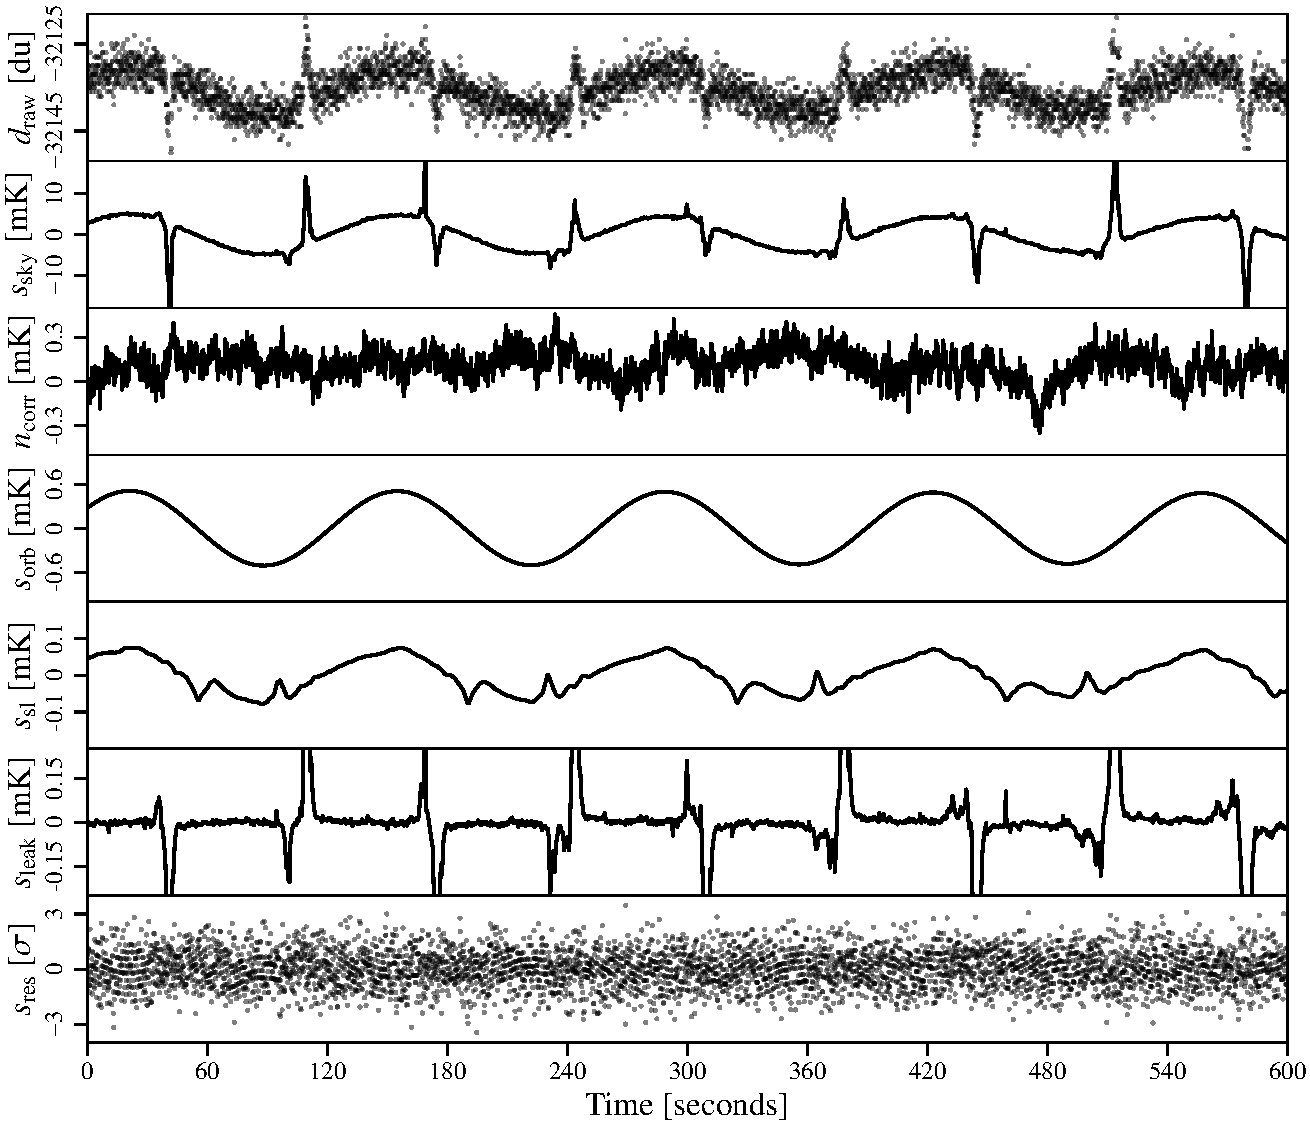
\includegraphics[width=\textwidth]{figures/K113_timestreams.pdf}
	\caption{Time-ordered data segment for the \K113 radiometer. From top to bottom, the panels show 1) raw uncalibrated TOD $\boldsymbol d$; 2) sky signal $\boldsymbol s_\mathrm{sky}$; 3) calibrated correlated noise $\boldsymbol n_\mathrm{corr}$; 4) orbital CMB dipole signal $\boldsymbol s_\mathrm{orb}$; 5) sidelobe correction $\boldsymbol s_\mathrm{sl}$; 6) bandpass leakage correction $\boldsymbol s_\mathrm{leak}$; and 7) residual TOD, $\boldsymbol d_\mathrm{res}=(\boldsymbol d -\boldsymbol n_\mathrm{corr}-\boldsymbol b)/g-\boldsymbol s_\mathrm{sky}-\boldsymbol s_\mathrm{orb}-\boldsymbol s_\mathrm{leak} -\boldsymbol s_\mathrm{sl}$, in units of $\sigma_0[\mathrm{du}]$ for this TOD segment. Note that the vertical range varies significantly from panel to panel.
		}
	\label{fig:timestreams}
\end{figure*}

Perhaps the most fundamental difference between the \commander\ and \WMAP\ (and those of most other CMB experiments) analysis pipelines is that while the \WMAP\ pipeline models each channel in isolation, the \cosmoglobe\ framework simultaneously considers all data, both internally within \WMAP, and also from all other sources, most notably also including \Planck. The main advantage of such a global approach is significantly reduced parameter degeneracies, as data from observations with different frequency coverages and instrumental designs break the same degeneracies. For this approach to be computationally tractable, one must establish a global parametric model that simultaneously accounts for both the astrophysical sky and all relevant instruments. For the current \WMAP+LFI oriented analysis, we adopt the following expression \citep{bp01},
\begin{equation}
	\label{eq:model}
	\boldsymbol d =\mathsf G\mathsf P[\mathsf B^\mathrm{symm}\mathsf M\boldsymbol a+\mathsf B^\mathrm{4\pi}(\boldsymbol s^\mathrm{orb}
	+\boldsymbol s^\mathrm{fsl})] + \boldsymbol s^\mathrm{inst}+ \boldsymbol n^\mathrm{corr}+\boldsymbol n^\mathrm w,
\end{equation}
where $\mathsf G$ is the time-dependent gain in the form of the matrix $\mathrm{diag}(g_t)$; $\mathsf P$ is the $n_p\times n_t$ pointing matrix, where $n_p$ is the number of pixels and $n_t$ the number of TOD datapoints;
$\mathsf B^\mathrm{symm}$ and $\mathsf B^{4\pi}$ are the symmetrized and full asymmetric beam, respectively; $\mathsf M$ is the mixing matrix between a given component $c$ with spectral energy distribution $f_c(\nu/\nu_{0,c})$ and a detector $j$ with bandpass $\tau_j(\nu)$, given by
\begin{equation}
	\mathsf M_{cj}=\int d\nu\,\tau_j(\nu)f_c(\nu/\nu_{c,0}).
\end{equation}
The maps $\boldsymbol a$ represent the Stokes parameters for each astrophysical component, while $\boldsymbol s^\mathrm{orb}$ is the orbital dipole induced by the motion of the telescope with respect to the Sun, and $\boldsymbol s^\mathrm{fsl}$ is the time-dependent far sidelobe signal. Following \citet{bp06}, we model the correlated noise component $\boldsymbol n^\mathrm{corr}$ in terms of a $1/f$ power spectral density (PSD), which explicitly takes the form $P_\mathrm{n}(f) = \sigma^2_0 (1 + (f/f_\mathrm{k})^\alpha)$, where $\sigma_0$ denotes the white noise amplitude, $f_\mathrm{knee}$ is the so-called $1/f$ knee frequency, and $\alpha$ is a free power law slope. For notational purposes, we denote the set of all correlated noise parameters by $\xi_{\mathrm{n}} = \{\sigma_0, f_{\mathrm{k}}, \alpha\}$. We note that this model represents a significant approximation, as the actual \WMAP\ noise is known to exhibit a significantly colored noise at high temporal frequencies. The main impact of this approximation is a worse-than-expected $\chi^2$ goodness-of-fit statistic. However, measured in absolute noise levels the effect is very small, and has very little if any impact on the final science results; for further discussion of this approximation, see Sect.~\ref{sec:noisemodel}. 

The term $\boldsymbol s^\mathrm{inst}$ denotes any instrument-specific terms that might be required for a given experiment. For instance, for LFI it is used to model the 1\,Hz spike contribution due to electronic cross-talk. For \WMAP, we use it for first-order baseline corrections, and set $s^\mathrm{WMAP}_t = b_0 + b_1\,t$, where $b_0$ and $b_1$ represent the mean and slope of the baselines over the data segment in question. We note that while the \WMAP\ team fitted a single constant baseline over either 1- or 24-hour periods, our data segments are typically about 3\,days long (corresponding to a number of samples that is an exact power of 2 to optimize Fourier transforms). A natural question is therefore whether non-linear baseline variations could induce artefacts. In this regard, it is important to note that the correlated noise component effectively acts as a single-sample baseline correction that can absorbe by far most such non-linearities, as long as their total effect on the power spectrum does not exceed that imposed by the $1/f$ model. In practice, that is a very mild constraint. At the same time, visual inspection of $\n^{\mathrm{corr}}$ projected into sky maps provides a very powerful check on any potential baseline residuals; these will appear as correlated stripes aligned with the \WMAP\ scanning path. In sum, it is important to note that \cosmoglobe\ model allows for a more flexible baseline behaviour than the \WMAP\ pipeline.

A third notable difference between the \WMAP\ and \cosmoglobe\ data models concerns bandpass mismatch. While the \WMAP\ pipeline simply projects out any bandpass difference from the polarization maps by solving for the spurious $S$ maps, we model it explicitly through the use of the global astrophysical sky model \citep{bp09}. Explicitly, the expected calibrated sky signal for radiometer $j$ is given by
\begin{equation}
	m_{p,j}=\mathsf B_{p,p'}\sum_c\mathsf M_{c,j}a^c_{p'}+n_{j,p}^\mathrm w.
\end{equation}
Since $\mathsf M_{c,j}$ encodes the bandpass response of every detector $j$ to every sky component $c$, the detector-specific maps, $\boldsymbol m_j$, will each be slightly different depending on their bandpass $\tau_j$. Therefore, before averaging different detectors together, we estimate the average over all detectors in a given frequency channel $\boldsymbol m\equiv \langle \boldsymbol m_j\rangle$, and subtracts it directly in the timestream;
\begin{equation}
	\delta s_{t,j}^\mathrm{leak}=\mathsf P_{t,p}^j\mathsf B_{p,p'}^j\left(\boldsymbol m_{j,p'}-\boldsymbol m_{p'}\right).
\end{equation}
This leakage term uses the expected bandpass response to remove the expected component that deviates from the mean in the timestream, directly reducing polarization contamination. 

To build intuition regarding this model, we plot in Fig.~\ref{fig:timestreams} both the TOD and the individual model components for an arbitrarily selected ten-minute segment for the \WMAP's \K113 radiometer. The uncalibrated data, $\boldsymbol d_\mathrm{raw}$, is displayed in the top panel, with the sky signal $\boldsymbol s_\mathrm{sky}=\mathsf P\mathsf B^\mathrm{symm}\mathsf M\boldsymbol a$ plotted directly underneath. The next four panels show the correlated noise realization $\boldsymbol n_\mathrm{corr}$, the orbital dipole $\boldsymbol s_\mathrm{orb}$, the far sidelobe contribution $\boldsymbol s_\mathrm{sl}$, and the bandpass leakage $\boldsymbol s_\mathrm{leak}$. Finally, we also plot the time-ordered residual for this segment of data, obtained by subtracting the model from the raw data, in units of the estimated white noise level. 


\subsection{Sky model}\label{subsec:sky_model}

Following \citet{bp01}, we assume that the sky (as defined by $\M\boldsymbol a$ in Eq.~\ref{eq:model}) across the \WMAP\ frequencies can be modeled as a linear combination of CMB fluctuations ($\vec{a}_{\mathrm{CMB}}$), synchrotron ($\vec{a}_{\mathrm{s}}$), free-free emission ($\vec{a}_{\mathrm{ff}}$), anomalous microwave emission ($\vec{a}_{\mathrm{ame}}$), thermal dust ($\vec{a}_{\mathrm{d}}$), and radio point sources ($\vec{a}_{j,\mathrm{src}}$). Explicitly, we assume that the astrophysical sky (in units of brightness temperature) may be modelled as follows,
\begin{align}
  \vec{s}_{\mathrm{RJ}} &= \left(\vec{a}_{\mathrm{CMB}}+\vec{a}_{\mathrm{quad}}(\nu)\right) \frac{x^2 \e^x}{(\e^x -1)^2}+\label{eq:cmb_astsky}\\
  &+ \vec{a}_{\mathrm{s}} \left(\frac{\nu}{\nuzeros}\right)^{\bsynch} + \label{eq:synch_astsky}\\
  &+ \vec{a}_{\mathrm{ff}} \left(\frac{\nuzeroff}{\nu}\right)^2 \frac{g_{\mathrm{ff}}(\nu;\Te) }{g_{\mathrm{ff}}(\nuzeroff;\Te)} +\label{eq:ff_astsky}\\
  %&+ \vec{a}_{\mathrm{ame}} \left(\frac{\nuzeroame}{\nu}\right)^2 \frac{f_{\mathrm{ame}} \left(\nu\cdot \frac{30.0\,\mathrm{GHz}}{\nup}\right)}{f_{\mathrm{ame}} \left(\nuzeroame\cdot \frac{30.0\,\mathrm{GHz}}{\nup}\right)}+\label{eq:ame_astsky}  \\
  &+ \vec{a}_{\mathrm{ame}} \e^{\beta_{\mathrm{AME}}(\nu-\nu_{0,\mathrm{ame}})}+\label{eq:ame_astsky}  \\
  &+ \vec{a}_{\mathrm{d}} \left(\frac{\nu}{\nuzerod}\right)^{\bdust+1} \frac{\e^{h\nuzerod/\kB\Tdust}-1}{\e^{h\nu/\kB\Tdust}-1}+ \label{eq:dust_astsky}\\
  &+ U_{\mathrm{mJy}} \sum_{j=1}^{N_{\mathrm{src}}} \vec{a}_{j,\mathrm{src}} \left(\frac{\nu}{\nuzerosrc}\right)^{\alpha_{j,\mathrm{src}}-2}, \label{eq:sum_ptsrc}
\end{align}
where $x=h\nu/kT_{\mathrm{CMB}}$; $\nu_{0,i}$ is a reference frequency for component $i$; $\beta_{\mathrm{s}}$ is a power-law index for synchrotron emission (which may take different values for temperature and polarization); $T_e$ is the electron temperature, and $g_{\mathrm{ff}}$ is the so-called Gaunt factor \citet{dickinson2003}; $\beta_{\mathrm{AME}}$ is an exponential scale factor for AME emission (see below); $\beta_{\mathrm{d}}$ and $T_{\mathrm{d}}$ are the emissitivity and temperature parameters for a single modified blackbody thermal dust model; $\alpha_{j,\mathrm{sr}}$ is the spectral index of point source $j$ relative to the same source catalog as used by \citet{planck2016-l04}; and $U_{\mathrm{mJy}}$ is the conversion factor between flux density (in millijansky) and brightness temperature (in $K_{\mathrm{RJ}}$) for the channel in question. Also, $\a_{\mathrm{quad}}$ accounts for a relativistic quadrupole correction due to the Earth's motion through space \citep{Notari:2015}.

In general, this model is nearly identical to the one adopted by \citet{bp01}. However, there is one notable exception, namely the spectral energy density (SED) for the AME component, $\boldsymbol s_0^\mathrm{sd}(\nu)$. In this current work, we adopt a simple exponential function for this component, as for instance proposed by \citet{hensley:2015}, which is notably different from the \texttt{SpDust2} model \citep{ali-haimoud:2009, ali-haimoud:2010, silsbee:2011} that was used in the \bp\ analysis. The motivation for this modification is discussed in detail by \citet{watts2023_ame}: First and foremost, the current combination of \WMAP\ and LFI data appears to prefer a higher signal amplitude at frequencies between 40 and 60\,GHz than can easily supported by \texttt{SpDust2}. This was first noted by \citet{planck2014-a11}, who solved this issue by introducing a second independent AME component. For the original \bp\ analysis, on the other hand, this excess was not statistically significant, simply because that analysis did not include the powerful \WMAP\ \K-band data. In the current analysis, the excess is obvious. The observation that a simple one-parameter exponential model fits the data as well as the complicated multi-parameter model of \citet{planck2014-a11} is a novel result from the current work. Indeed, it fits also about as well as the commonly used log-normal model derived by \citet{Stevenson_2014}, which also has one extra parameter. By virtue of having fewer degrees of freedom than any of the previous models, we adopt the exponential model in the following.

%, the simple exponential model has one fewer parameter than the often-used phenomenological log-normal model, while also appearing to perform at least roughly equally well for the current data. At the same time, it is obvious that the exponential model cannot be extrapolated to lower frequencies, and the \cosmoglobe\ model presented here is therefore only applicable to data at frequencies higher than 23\,\GHz. (For lower-frequency data used in the following, namely the Haslam 408\,MHz observations, we set the AME amplitude to zero by hand.)

%\citet{bp01} by a peak frequency $\nu_\mathrm p$ such that
%\begin{equation}
%	s^\mathrm{sd}_\mathrm{RJ}(\nu)\propto\nu^{-2}\boldsymbol s_0^\mathrm{sd}\left(\nu\cdot\frac{30\,\mathrm{GHz}}{\nu_\mathrm p}\right).
%\end{equation}
%In the \WMAP\ and LFI frequency range, the exponential model and the \texttt{SpDust2} are phenomenologically quite similar, despite their very different descriptions. 
%As we describe in (\ldots), 
%The exponential model is a simple fit with $\beta$ drawn from a prior value of $-3.57$, and is a clear parametric form that is easy to interpret. An alternative model is the two-parameter log-normal AME SED,
%\begin{equation}
%	\boldsymbol s_\mathrm{RJ}^\textrm{ame,log-N}=\boldsymbol a_\mathrm{ame}
%	\left(\frac{\nu}{\nu_\mathrm{ame}}\right)^{-2}\exp\left(-\frac12\left[\frac{\ln(\nu/\nu_\mathrm{ame})}{W_\mathrm{ame}}\right]^2\right),
%\end{equation}
%derived by \citet{Stevenson_2014} as an analytical approximation to the spinning dust emission. This has also been employed in the latest QUIJOTE analaysis, e.g., \citet{QUIJOTE_V}, as it allows for variation of the peak frequency $\nu_\mathrm{ame}$ and width $W_\mathrm{ame}$. Although this work is not dependent on the specific parametric form of the AME, we opt for the exponential form described above, as it provides an excellent fit to the diffuse AME with a single parameter.

%\begin{figure}
%	\centering
%	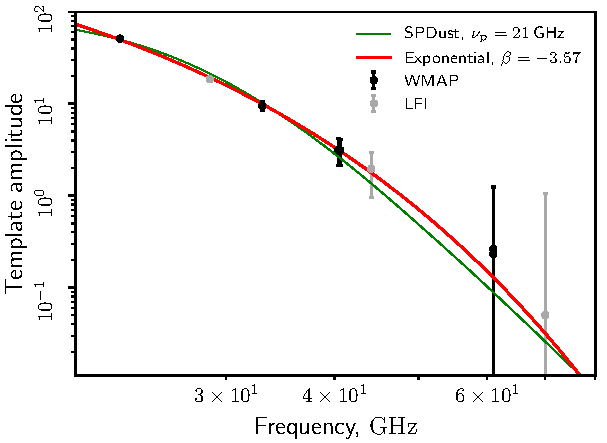
\includegraphics[width=\linewidth]{figures/tempfit_AME_single_v1.pdf}
%	\caption{AME exponential}
%\end{figure}

\subsection{Priors and poorly measured modes}
\label{sec:priors}

\begin{figure}
	\centering
	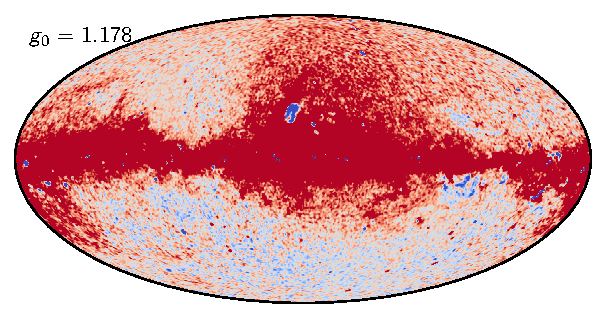
\includegraphics[width=\columnwidth]{figures/ame_g01_178.pdf}
	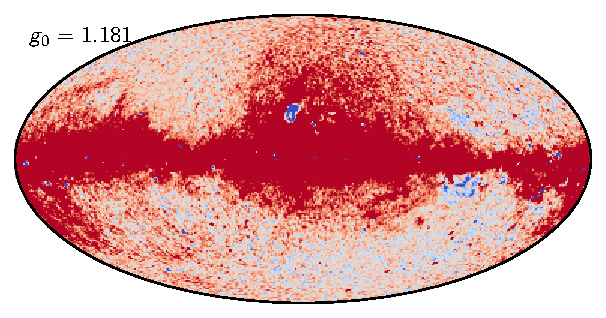
\includegraphics[width=\columnwidth]{figures/ame_g01_181.pdf}
	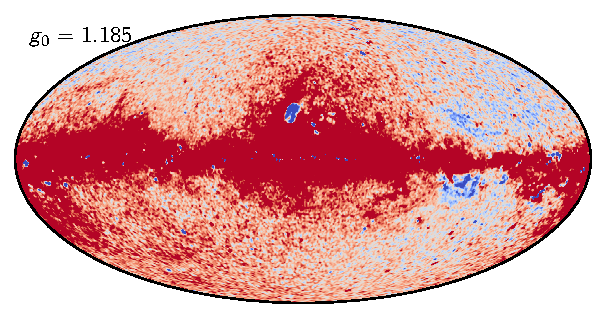
\includegraphics[width=\columnwidth]{figures/ame_g01_185.pdf}
	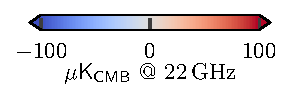
\includegraphics[width=0.5\columnwidth]{figures/cbar_100uK.pdf}
	\caption{Dependence on AME amplitude evaluated at 22\,GHz as a function of absolute calibration. Each map comes from the fifth iteration of a dedicated \commander\ run that fixed $g_0$ while letting all other TOD parameters be fit. The values of $g_0=1.178$ and $g_0=1.185$ represent $3.5\sigma$ draws from the prior distribution with mean $1.1815$ and standard deviation $0.001$. The dipole visible in the top and bottom panels is aligned perfectly with the Solar dipole, and is directly due to variations in the \K-band absolute calibration.}
	\label{fig:g0_ame}
\end{figure}

The model described in Sects.~\ref{sec:wmap_instmodel} and \ref{subsec:sky_model} is prone to several degeneracies, allowing for unphysical solutions to be explored in the Gibbs chain. Such unphysical degeneracies are highly undesirable for two main reasons. First, they increase the statistical uncertainties on most (if not all) other important parameters in the model --- sometimes to the point that the target quantity is rendered entirely unmeasurable. Secondly, and perhaps even more importantly, the data model described above is known to be a (sometimes crude) approximation to the real observations, and there will invariably be modelling errors. Degeneracies then generally tend to amplify their impact, in the sense that any unconstrained parameters will typically be used to fit such small modelling errors. For both these reasons, it is generally preferrable to impose either informative or algorithmic priors on the unconstrained parametes, rather than to leave them entirely unconstrained in the model.

An important example of an algorithmic prior is the foreground smoothing prior used by \citet{planck2016-l04,bp12}, which dictates that astrophysical foregrounds has to be smooth on small angular scales. This is justified by noting that the angular spectrum on large and intermediate scales typically falls as a power-law in multipole space; extrapolating this into the noise dominated regime prevents the overall foreground model from becoming degenerate at small scales.

Correspondingly, important examples of informative priors are the use of HFI constraints on the thermal dust SED parameters, $\beta_{\mathrm{d}}$ and $T_{\mathrm{d}}$ in \bp. Because that analysis only included the highest HFI frequency channels, they had very little constraining power on the thermal dust SED. Rather than trying to fit these directly from LFI \WMAP\ alone, they instead imposed informative Gaussian priors on each of these parameters, as derived from the HFI observations \citep{planck2016-l04}.

In the current analysis, and unless otherwise noted, we adopt the same algorithmic and informative priors as \citet{bp01}. However, there are three notable exceptions, as detailed below, all of which are dictated either by the fact that we include the \WMAP\ \K-band channel (which has a strong impact on the low-frequency foreground model), or by the fact that we now process the \WMAP\ data in time-domain, and therefore are subject to the same degeneracies as the official \WMAP\ low-level pipeline, and that were solved with similar implicit or explicit prior in the original analysis.

First and foremost, and as detailed in Sect.~\ref{sec:ame_Kband}, we observe in the current analysis a very strong degeneracy between the absolute calibration of the \K-band channel and the dipole of the AME map. This makes intuitively sense, since \K-band is by far the strongest channel in terms of AME signal-to-noise ratio, exceeding that of LFI 30\,GHz by about a factor of four; see Sect.~\ref{sec:s2n}. Effectively, a small variation in the absolute gain may be countered by subtracting corresponding CMB Solar dipole variation from the AME map, and end up with a nearly identical total $\chi^2$; the orbital CMB dipole is not bright enough at 23\,GHz relative to AME emission to break this degeneracy.

This is illustrated in Fig.~\ref{fig:g0_ame}, which shows the derived AME amplitude map for three different values of the mean \K-band gain, $g_0$, namely 1.178, 1.181, and $1.184\,\mathrm{du\,mK^{-1}}$; the extreme values differ only by 0.25\,\%. All of these three values appear equally acceptable from a pure $\chi^2$ point-of-view, relative to the noise level and modelling errors of these data. At the same time, it is obviously clear from visual inspection that only the middle value actually makes physical sense, as compared to what we know about the structure of the Milky Way. For this reason, we apply a Gaussian prior on the absolute \K-band gain of $g_0 \sim \mathcal N(1.181, 0.001^2)$ in the following, to regularize this issue. Thus, the extreme panels in Fig.~\ref{fig:g0_ame} represent $\pm2.5\,\sigma$ outliers, respectively, and will appear in our Markov chains with a frequency of about 1-in-100.

It is reasonable to ask why the \WMAP\ pipeline produced sensible results without applying such a prior during their calibration procedure. It is then important to recall the main difference between the two approaches: While \cosmoglobe\ attempts to fit a single overall parametric model to all data at once, the \WMAP\ pipeline calibrated each channel independently by co-adding data from one channel into a map; subtracting that map from the TOD; fitting the gain to the orbital dipole; and iterating until the solution became stable. An obvious advantage of such a single-channel approach is that the solution is independent of the assumed sky model. However, an equally obvious disadvantage is that it is impossible to break any potential inherent degeneracies with that approach; it cannot be combined with external observations in any meaningful way. And one important degeneracy for the \WMAP\ data is a strong degeneracy between the transmission imbalance factors and the polarized sky signal; it is exceedingly difficult to break this degeneracy using data from only one radiometer alone, and the resulting errors will propagate to most other aspects in the analysis. In the global approach, on the other hand, the polarization modes that are poorly measured by \WMAP\ alone are well measured by \Planck, and the result is an overall better fit. 

Second, as reported by \citet{bp14} for the \BP\ analysis, another important degeneracy in the current global model concerns the spectral index of polarized synchrotron emission versus the time-variable detector gain; when fitting both the polarized synchrotron amplitude and calibration freely without priors, the synchrotron spectral index at high Galactic latitudes tend to be biased toward unreasonably flat values, $\beta \lesssim -2.5$, which was likely due to a low level of unmodelled systematics, for instance temperature-to-polarization leakage, rather than true polarized synchrotron emission. In turn, this resulted in a clearly contaminated CMB sky map with a strong synchrotron morphology. To break this degeneracy, \citet{bp14} chose to marginalize the high-latitude synchrotron spectral index over a Gaussian prior of $N(-3.30,0.1^2)$, informed by \citet{planck2016-l05}, rather than estimate it from the data themselves. In the current analysis, we observe the same degeneracy, and the introduction of the \K-band data is not sufficient to break it on its own. For this reason, we choose to apply the same informative prior in the current analysis.

Third and finally, we also marginalize over the AME scale index with a prior of $\beta_{\mathrm{AME}}=N(3.56, 0.1)$. The parameters of these priors were determined by running a grid over $\beta_{\mathrm{AME}}$, and identifying the range that resulted in reasonable residuals near the Galactic plane, similar to that shown in Fig.~\ref{fig:g0_ame} for the absolute calibration of \K-band. We note that this prior should in principle be replaced with direct $\chi^2$-based posterior optimization, combined with a properly tailored analysis mask. However, the recent release of the QUIJOTE data \citep{QUIJOTE_IV}, which covers the all-important 11--19\,GHz frequency range, suggests that the entire AME model should be revisited in a future joint \WMAP+LFI+QUIJOTE analysis, and we therefore leave detailed prior and SED optimization to that work. For further information regarding AME modelling with the current dataset, we refer the interested reader to \citet{watts2023_ame}.

\subsection{Posterior distribution and Gibbs sampling}

As shown by \citet{bp01}, this joint parametric description of the instrumental effects and sky allows us to write down a total model for the data, $\boldsymbol d=\boldsymbol s^\mathrm{tot}(\boldsymbol\omega)+\boldsymbol n^\mathrm w$, where $\boldsymbol s^\mathrm{tot}$ encompasses all of the terms in Eq.~\eqref{eq:model} except for the white noise term. Assuming that all instrumental effects have been modeled adequately, and that the white noise is Gaussian distributed, the data should then also be Gaussian distributed with a mean of $\boldsymbol s^\mathrm{tot}(\boldsymbol\omega)$ and variance $\boldsymbol \sigma_0^2$. In general, the likelihood reads
\begin{equation}
	P(\boldsymbol d\mid\boldsymbol\omega)\propto\exp\left(-\frac12\sum_t\frac{(d_t-s^\mathrm{tot}_t(\boldsymbol\omega))^2}{\sigma_0^2}
	\right).
\end{equation}
If $\boldsymbol d\sim\mathcal N(\boldsymbol s^\mathrm{tot},\boldsymbol\sigma_0^2)$ is the correct model for the data, the argument of the exponent is proportional to a $\chi^2$-distribution with $n_\mathrm{TOD}$ degrees of freedom. In the limit of large $n$, a $\chi^2$ distribution is well-approximated by a Gaussian with mean $n$ and variance $2n$. Therefore we define and use in the following the reduced normalized $\chi^2$ statistic,
\begin{equation}
	\chi^2\equiv \frac{\sum_t((d_t-s_t^\mathrm{tot})^2/\sigma_0^2 - n_\mathrm{TOD}}{\sqrt{2n_\mathrm{TOD}}},
\end{equation}
which is approximately drawn from the standard normal distribution $\mathcal N(0,1)$.

Following \citet{bp01}, the \cosmoglobe\ Gibbs chain for this analysis is given by
\begin{alignat}{10}
\label{eq:gain_samp_dist}\g &\,\leftarrow          P(\g&\,               \mid \data, &\,    &          &\,\boldsymbol\xi_n,  &\,\boldsymbol s^\mathrm{inst}, &\,\boldsymbol\beta, &\,\boldsymbol a, &\,C_{\ell},&\,\boldsymbol\theta)\\
\label{eq:ncorr_samp_dist} \ncorr &\,\leftarrow    P(\ncorr&\,           \mid \data, &\,\g, &\,        &\,\boldsymbol\xi_n,  &\,\boldsymbol s^\mathrm{inst}, &\,\boldsymbol\beta, &\,\boldsymbol a, &\,C_{\ell},&\,\boldsymbol\theta)\\ 
\label{eq:xi_samp_dist} \boldsymbol\xi_n &\,\leftarrow        P(\boldsymbol\xi_n&\,            \mid \data, &\,\g, &\,\ncorr, &\,        &\,\boldsymbol s^\mathrm{inst}, &\,\boldsymbol\beta, &\,\boldsymbol a, &\,C_{\ell},&\,\boldsymbol\theta)\\
\label{eq:samp_inst}\boldsymbol s^\mathrm{inst} &\,\leftarrow                                 P(\boldsymbol s^\mathrm{inst}&\,             \mid \data, &\,\g, &\,\ncorr, &\,\boldsymbol\xi_n,  &\,      &\,\boldsymbol\beta, &\,\boldsymbol a, &\,C_{\ell},&\,\boldsymbol\theta)\\
\label{eq:beta_samp}\boldsymbol\beta &\,\leftarrow                     P(\boldsymbol\beta&\, \mid \data, &\,\g, &\,\ncorr, &\,\boldsymbol\xi_n,  &\,\boldsymbol s^\mathrm{inst}, &\,       &\,    &\,C_{\ell},&\,\boldsymbol\theta)\\
\boldsymbol a &\,\leftarrow                                   P(\boldsymbol a&\,               \mid \data, &\,\g, &\,\ncorr, &\,\boldsymbol\xi_n,  &\,\boldsymbol s^\mathrm{inst}, &\,\boldsymbol\beta, &\,    &\,C_{\ell},&\,\boldsymbol\theta)\\
C_{\ell} &\,\leftarrow                             P(C_{\ell}&\,         \mid \data, &\,\g, &\,\ncorr, &\,\boldsymbol\xi_n,  &\,\boldsymbol s^\mathrm{inst}, &\,\boldsymbol\beta, &\,\boldsymbol a,&\,\phantom{C_{\ell}}&\,\boldsymbol\theta)&\label{eq:cl_sampling}\\
\boldsymbol\theta &\,\leftarrow                             P(\boldsymbol\theta&\,         \mid \data, &\,\g, &\,\ncorr, &\,\boldsymbol\xi_n,  &\,\boldsymbol s^\mathrm{inst}, &\,\boldsymbol\beta, &\,\boldsymbol a,&\,C_\ell\phantom{,}&\,\phantom{\boldsymbol\theta})\label{eq:param_samp},
\end{alignat}
with each step requiring its own dedicated sampling algorithm. The \commanderthree\ pipeline is designed so that results of each Gibbs sample can be easily passed to each other, and that the internal calculations of each step do not directly depend on the inner workings of each other, which greatly increases modularity of the code. 

%MG: not sure this bit is particularily relevant for this paper, feel free to overrule me
%To add another data set to the Gibbs chain, one can either add a map or TODs. To add a TOD, one must implement Eqs.~\eqref{eq:gain_samp_dist}--\eqref{eq:samp_inst} for each instrument, as was done in \citet{bp01} and \citet{bp10} for \Planck\ LFI and in \citet{bp17} for \WMAP. To add a map, one must simply pass processed maps with beam, mask, and noise information to Eqs.~\eqref{eq:beta_samp}--\eqref{eq:param_samp}, as was done for the Haslam 408\,MHz map \citep{haslam1982,remazeilles2014} and the \Planck\ 353 and 857\,GHz maps.





\subsection{Sampling algorithms}
\label{sec:algorithms}

Before we discuss the results of this Gibbs chain as applied to the \Planck\ LFI and \WMAP\ data, we summarize the TOD processing steps in this section. Each step of the Gibbs chain requires its own conditional distribution sampling algorithm. In Sect.~\ref{ssec:oldsamplers} we review the sampling algorithms implemented in the \bp\ suite of papers, while Sects.~\ref{ssec:mapmaking}--\ref{ssec:baseline} provide an overview of the \WMAP-specific processing steps.

\subsubsection{Review of sampling algorithms}
\label{ssec:oldsamplers}


By far most of the techniques required for \WMAP\ data analysis have already been  described in the \bp\ project and implemented in \commanderthree. This section includes a summary of the algorithms that were used previously for the analysis of LFI data. In each of these cases, every part of the model not explicitly mentioned is held fixed unless specified otherwise.

Noise estimation and calibration are described by \citet{bp06} and \citet{bp07}, respectively. As noted in those works, these two steps are strongly correlated, simply because the timestream
\begin{equation}
	d_{t,i}=g_{q,i}s_{t,i}^\mathrm{tot}+n_{t,i}^\mathrm{corr}+n_{t,i}^\mathrm{wn}
\end{equation}
may be almost equally well fit by two solutions defined by $g'=gs^\mathrm{tot}/(s^\mathrm{tot})'$ or ${(n^\mathrm{corr})'=n^\mathrm{corr}+gs^\mathrm{tot}+g'(s^\mathrm{tot})'}$; the only thing that breaks this degeneracy is the noise PSD, which is a relatively loose constraint. A Gibbs sampler is by nature not very effective for nearly degenerate distributions, and we therefore instead define a joint sampling step for the correlated noise and gain. In practice, this is done by first drawing the calibration from its marginal distribution with respect to $\boldsymbol n^\mathrm{corr}$, and then drawing $\boldsymbol n^\mathrm{corr}$ from its conditional distribution with respect to $g$,
\begin{alignat}{10}
	\g&\,\leftarrow P(\g&\,\mid\data, &\, &\,&\,\boldsymbol\xi_n,\ldots)
	\label{eq:gmarg}
	\\
	\ncorr&\,\leftarrow P(\ncorr&\,\mid\data, &\,\g, &\,&\,\boldsymbol\xi_n,\ldots).
	\label{eq:ncorr_only}
\end{alignat}
It is easy to see that this is a valid sample from the joint distribution sipmly from the defintion of a conditional distribution, $P(\g,\ncorr\mid\boldsymbol\omega)=P(\ncorr\mid\g,\boldsymbol\omega)P(\g\mid\boldsymbol\omega)$. In practice, this simply means that when sampling for $\g$, the covariance matrix $\mathsf N=\mathsf N_\textrm{wn}+\mathsf N_\textrm{corr}$ must be used, rather than just $\mathsf N_\mathrm{wn}$.

\commanderthree\ models the gain at each timesteam $t$ for a detector $i$ as
\begin{equation}
	g_{t,i}=g_0+\Delta g_i+\delta g_{q,i}
\end{equation}
where $q$ labels the time interval for which we assume the gain is constant, typically a single scan. In order to sample the gain, we write down a generative model for the TOD,
\begin{equation}
	\dv_i=\g_{i}\s_{i}^\mathrm{tot} +\n_{i}^\mathrm{tot}\sim\mathcal N(\g_i\s_{i}^\mathrm{tot},\mathsf N_i).
\end{equation}
Since the $\dv_i$ is given as a linear combination of the fixed signal and the gains, a random sample of the gain can be drawn by solving\footnote{See, e.g., Appendix A.2 of \citet{bp01} for a derivation of this result.}
\begin{equation}
	\label{eq:gain_gauss_samp}
	[(\s_i^\mathrm{tot})^T\mathsf N_i^{-1}\s_i^\mathrm{tot}]\g_i
	=(\s_i^\mathrm{tot})^T\N^{-1}_i\dv_i
	+(\s_i^\mathrm{tot})^T\N^{-1/2}_i\boldsymbol\eta.
\end{equation}
Note that the $\mathsf N_i$ depends implicitly on the noise PSD $\boldsymbol \xi_n$, while the specific realization of $\ncorr$ is accounted for in the covariance matrix.
As detailed by \citet{bp07}, \commanderthree\ samples in practice $g_0$, $\Delta g_i$, and $\delta g_{q,i}$ in separate sampling steps. Specifically, the absolute calibration $g_0$ is for the CMB-dominated channels only fitted using the orbital dipole, while the relative calibrations, $\Delta g_i$, exploits the full sky signal. The same is true for the time-dependent gain fluctuations, $\delta g_{q,i}$, and in this casee an additional smoothness prior is applied through an effective Wiener filter. It is worth noting that the Gibbs chain is formally broken by fitting the absolute gain $g_0$ to the orbital dipole alone, as opposed to the full sky signal. However, this makes the sampling more robust with respect to unmodeled systematic effects, somewhat analogous to applying a confidence mask when estimating the CMB power spectrum.

The correlated noise sampling, described by \citet{bp06}, follows a similar procedure, except this now conditions upon the previous gain estimate, which is sampled immediately before the correlated noise component in the code. Similar to the gain case, we can write a generative model for the data,
\begin{equation}
	\dv_i=\g_i\s_i^\mathrm{tot}+\n_i^\mathrm{corr}+\n^\mathrm{wn}_i
	\sim\mathcal N(\g_i\s_i^\mathrm{tot},\N_{\mathrm{corr},i}+\N_{\mathrm{wn},i}).
\end{equation}
Given fixed $\boldsymbol r_i=\dv_i-\g_i\s_i^\mathrm{tot}$, we can again write a sampling equation, 
\begin{equation}
	\label{eq:ncorr_gauss_samp}
	(\N_{\mathrm{corr},i}^{-1}+\N_{\mathrm{wn},i}^{-1})
	\n^\mathrm{corr}_i
	=\N^{-1}_{\mathrm{wn},i}\boldsymbol r_i
	+\N^{-1/2}_{\mathrm{wn},i}\boldsymbol\eta_1
	+\N^{-1/2}_{\mathrm{corr},i}\boldsymbol\eta_2.
\end{equation}
This gives a sample of the underlying correlated noise. %In practice, this is equivalent to the destriping mapmaking algorithm \texttt{Madam}, and returns equivalent results to the classical method \citep{bp02}.

To sample the correlated noise parameters, we assume that the correlated noise is drawn from a correlated Gaussian and form the conditional posterior distribution,
\begin{equation}
	P(\boldsymbol\xi_n\mid\n^\mathrm{corr})\propto\frac{\exp{[-\frac12(\n^\mathrm{corr})^T\N_\mathrm{corr}^{-1}\n^\mathrm{corr}]}}
	{\sqrt{|\N_\mathrm{corr}|}}P(\boldsymbol\xi_n).
\end{equation}
The simplest and most commonly used parameterization for correlated noise is given by
\begin{equation}
	\mathsf N_\mathrm{corr}(f)=\sigma_0^2\left(\frac f{f_\mathrm{knee}}\right)^\alpha.
\end{equation}
This can in principal be modified, and for \Planck\ LFI a Gaussian log-normal bump was added at a late stage in the \bp\ analysis. Rather than sampling for $\sigma_0$, we effectively fix the white noise level to the noise level at the highest frequency, e.g.,
\begin{equation}
	\sigma_0^2\equiv\frac{\mathrm{Var}(r_{t+1}-r_t)}2,
\end{equation}
where $t$ and $t+1$ are consecutive time samples, and ${\boldsymbol r\equiv\boldsymbol d-\boldsymbol g\boldsymbol s^\mathrm{tot}
-\boldsymbol n^\mathrm{corr}}$. In practice, this makes $\sigma_0$ a deterministic function of the sampled sky and gain parameters. The parameters $\alpha$ and $f_\mathrm{knee}$ are not linear in the data, and they can be sampled efficiently using a standard inversion sampler (see, e.g., Appendix~A.3 of \citet{bp01} or Chapter~7.3.2 of \citet{numerical_recipes} for further details). In practice, this requires computing the posterior over a linear grid one parameter at a time.


Once the instrumental parameters have been sampled, \commanderthree\ computes the calibrated TOD for each band,
\begin{equation}
	r_{t,j}=\frac{d_{t,j}-n_{t,j}^\mathrm{corr}}{g_{t,j}}-\left(s_{t,j}^\mathrm{orb}
	+s_{t,j}^\mathrm{fsl}+\delta s_{t,j}^\mathrm{leak}+\vec{s}_{t,j}^\mathrm{inst}\right)
\end{equation}
where $\s^\mathrm{orb}$ is the orbital dipole \citep{bp07}, $\s^\mathrm{fsl}$ is the far sidelobe timestream \citep{bp08}, $\delta\s^\mathrm{leak}$ is the bandpass leakage \citep{bp09}, and $\s^\mathrm{inst}$ is some instrumental-specific contribution, e.g., the 1\,Hz electronic spike for LFI. With a correlated noise realization removed, one can perform simple binned mapmaking, weighting each pixel by the white noise amplitude.

% Component separation for intensity and polarization are described in \citet{bp13} and \citet{bp14}, respectively.

% Power spectrum estimation is described in \citet{bp12}.

% Cosmological parameter estimation is described in \citet{bp11}.


\subsubsection{Differential mapmaking}
\label{ssec:mapmaking}

The first additional algorithm that needs to be added to \commanderthree\ in order to process \WMAP\ TOD data is support for differential mapmaking \citep{bp17}. After calibration and correction for instrumental effects, the TOD can be modeled as
\begin{equation}
	\boldsymbol d=\mathsf P\boldsymbol m+\boldsymbol n^\mathrm{w},
\end{equation}
where
\begin{equation}
	\boldsymbol m=\mathsf B^\mathrm{symm}\mathsf M\boldsymbol a
\end{equation}
is the expected map for each detector after removing the orbital dipole, far sidelobe, baseline, and a realization of correlated noise. The differential pointing strategy can be represented in matrix form as 
\begin{align}
	\label{eq:wmap_pointing}
	\mathsf P_{tp}&=
	(1+x_\mathrm{im})(\delta_{p^I_{\phantom\A}p_\A^I}
	+\delta_{p^Q_{\phantom\A}p^Q_\A}\cos2\psi_\A
	+\delta_{p^U_{\phantom\A}p^U_\A}\sin2\psi_\A)
	\\
	&\quad-(1-x_\mathrm{im})(\delta_{p^I_{\phantom\B}p_\B^I}
	-\delta_{p^Q_{\phantom\A}p^Q_\B}\cos2\psi_\B
	-\delta_{p^U_{\phantom\A}p^U_\B}\sin2\psi_\B)\nonumber
\end{align}
where $p_\A$ and $p_\B$ are the time-dependent pointings for each DA. The maximum likelihood map can now in principle be derived using the usual mapmaking equation,
\begin{equation}
	\label{eq:mapmapking_eqn1}
	\mathsf P^T\mathsf N^{-1}\mathsf P\boldsymbol m=\mathsf P^T\mathsf N^{-1}\boldsymbol d.
\end{equation}
For a single-horn experiment, i.e., \Planck\ LFI, this reduces to a $3\times3$ matrix that can be inverted for each pixel independently. For the pointing matrix in Eq.~\eqref{eq:wmap_pointing}, this is no longer possible, as there is inherently coupling between horns A and B in the timestreams. The $3N_\mathrm{pix}\times3N_\mathrm{pix}$ matrix can be solved using an iterative algorithm, e.g., preconditioned conjugate gradients \citep{shewchuk:1994}.

\citet{jarosik2010} identified an issue where a large difference in the sky temperature values at pixel A versus pixel B induced artifacts in the mapmaking procedure. We adopt the procedure first described by \citet{hinshaw2003a} where only the pixel in a bright region, defined by a small processing mask \citep{bennett2012} is accumulated, thus modifying the mapmaking equation to
\begin{equation}
	\mathsf P^T_\mathrm{am}\mathsf N^{-1}\mathsf P\boldsymbol m
	=\mathsf P^T_\mathrm{am}\mathsf N^{-1}\boldsymbol d.
\end{equation}
This equation can be solved using the BiCG-STAB algorithm for a non-symmetric matrix $\mathsf A$ where $\mathsf A\boldsymbol x=\boldsymbol b$. We apply a preconditioner $\mathsf M$ by numerically inverting the same problem with $N_\mathrm{side}=16$ maps and applying a diagonal noise matrix. Numerically, we define convergence as when the residual $\boldsymbol r\equiv\boldsymbol b-\mathsf A\boldsymbol x$ satisfies $\boldsymbol r^T\mathsf M^{-1}\boldsymbol r/\boldsymbol b^T\mathsf M^{-1}\boldsymbol b<10^{-10}$, which typically takes about 20 iterations for producing frequency maps.


\subsubsection{Transmission imbalance estimation}
\label{ssec:imbalance}


Transmission imbalance, the differential power transmission of the optics and waveguide components, can be parameterized as
\begin{equation}
	d_{t,j}=g_{t,j}[(1+x_{\mathrm{im},j})s_{t,j}^\mathrm{tot,A}-(1-x_{\mathrm{im},j})s_{t,j}^\mathrm{tot,b}]+n_t.
\end{equation}
This can be decomposed into a differential (d) and common-mode (c) signal such that
\begin{equation}
	d_{t,j}=g_{t,j}[s_{t,j}^\mathrm d+x_{\mathrm{im},j}s_{t,j}^\mathrm c]+n_t.
\end{equation}
In this form, the imbalance parameters can be estimated by drawing Gaussian samples from the standard mean and standard deviation over the entire mission. To draw samples for $x_{\mathrm{im},j}$, we construct a sampling routine analogous to the gain estimation of Eq.~\eqref{eq:gain_gauss_samp} and correlated noise estimation of  \eqref{eq:ncorr_gauss_samp}, with $\boldsymbol r=\boldsymbol d-\boldsymbol g\boldsymbol s^\mathrm d$,
\begin{equation}
	[(\boldsymbol g\boldsymbol s^\mathrm c)^T\mathsf N^{-1}\boldsymbol g\boldsymbol s^\mathrm c]x_\mathrm{im}
	=(\boldsymbol g\boldsymbol s^\mathrm c)^T\mathsf N^{-1}\boldsymbol r+(\boldsymbol g\boldsymbol s^\mathrm c)^T\mathsf N^{-1/2}\boldsymbol\eta,
\end{equation}
essentially cross-correlating the common-mode signal with $\boldsymbol r$ with appropriate weights and adding a Gaussian random variable with the correct weighting. Note that we are marginalizing over the correlated noise here by using $\N=\N_\mathrm{wn}+\N_\mathrm{corr}$. This mitigates any baseline drifts being erroneusly attributed to the common-mode signal and biasing the estimate of $x_\mathrm{im}$.

The \WMAP\ procedure, described in \citet{jarosik2003a}, fit for common-mode and differential coefficients along with a cubic baseline over 10 precession periods at a time, corresponding to 10 hours of observation. The mean and uncertainty were then calculated by averaging and taking the standard deviation of these values. This approach has the benefit of allowing for the tracking of possible transmission imbalance variation throughout the mission. However, none of the \WMAP\ suite of papers have found evidence for this, and it has not arisen in our analysis, so we model this as an effect whose value is constant throughout the mission.

\subsubsection{Baseline sampling}
\label{ssec:baseline}

The data model adopted by \citet{hinshaw2003a} can be written in raw digital units (du) as
\begin{equation}
	\data = \mathsf{GPBM}\boldsymbol a+\boldsymbol n+\boldsymbol b,
\end{equation}
where $\boldsymbol b$ is the instrumental baseline and $\boldsymbol n$ is the
total instrumental noise. As noted above, \commanderthree\ divides
the noise into $\n=\n^\mathrm w+\n^\mathrm{corr}$, a white noise term and a
correlated noise term. By definition, the white noise does not have any
correlations between adjacent pixels, so that any pixel-pixel covariance should
be fully described by realizations of the $\n^\mathrm{corr}$ timestream.

\commander\ estimates the baseline using the full estimate of the current sky
model, $\boldsymbol r=\boldsymbol d-g\boldsymbol s^\mathrm{tot}=\boldsymbol
b+\boldsymbol n$. Modeling $\boldsymbol b=b_0+b_1\Delta t$, we solve for $b_0$
and $b_1$ using linear regression in each timestream while masking out samples
that lie within the processing mask. Strictly speaking, this is breaking the
Gibbs chain, as we are not formally sampling $b_0$ and $b_1$ for each TOD
chunk. In practice, baseline estimation uncertainty propagates to correlated
noise realizations and PSD parameters, as discussed below.

The approach detailed by \citet{hinshaw2003a} and the
\commander\ implementation differ mainly in two ways. First, the
assumed stable timescales are different --- the initial
\WMAP\ baseline is estimated over one hour timescales, and assumed to
be an actual constant, whereas \commander\ assumes constant values
throught the entire time chunk, which is 3--7 days depending on the
band in question, but allows a linear term in the baseline. Second,
the two methods differs in how they treat non-linear residuals in the
first-order baseline model.  As noted in \citet{hinshaw2003a},
residual baseline variations manifest as correlated noise stripes in
the final maps, and\WMAPnine\ solves this using a time-domain filter,
downweighting the data based off of the noise characterization. This
is fundamentally similar to the \commanderthree\ approach, which
accounts for this as part of the correlated noise component. The main
advantages of the latter is that it allows for proper error
propagation at all angular scales without the use of a dense
pixel-pixel noise covariance, and also that it provides a convenient
means for inspecting the residuals visually by binning the correlated
noise into a sky map.

\section{Data and data processing}
\label{sec:data}

\begin{table}
\caption{\cosmoglobe\ flagging statistics for each DA. The second column indicates the fraction of data that are removed by the official \WMAP\ flags, while the third column indicates the fraction that is additionally discarded in the current processing for computational reasons. The fourth column indicates the total fraction of data actually used to generate the final maps. }              % title of Table
\label{table:flagged_data}      % is used to refer this table in the text
\centering                                      % used for centering table
\begin{tabular}{c c c c}          % centered columns (4 columns)
\hline\hline                        % inserts double horizontal lines
	Band & Flagged (\%) & Discarded (\%) & Used (\%) \\    % table heading
\hline                                   % inserts single horizontal line
	\K  &  1.72 & 0.87 & 97.4\\
	\Ka &  1.64 & 0.88 & 97.5\\      % inserting body of the table
	\Q1 &  1.84 & 0.84 & 96.5\\
	\Q2 &  1.62 & 0.81 & 97.6\\
	\V1 &  1.62 & 1.10 & 97.3\\
	\V2 &  1.61 & 1.01 & 97.4\\
	\W1 &  1.76 & 1.03 & 97.2\\
	\W2 &  1.60 & 0.81 & 97.6\\
	\W3 &  1.61 & 0.87 & 97.5\\
	\W4 &  1.60 & 0.81 & 97.6\\
\hline                                             %inserts single line
\end{tabular}
\end{table}

\begin{table*}[t]
  \begingroup
  \newdimen\tblskip \tblskip=5pt
  \caption{Computational resources required for end-to-end
    \cosmoglobe\ processing. All times correspond to CPU hours, and all data volumes are reported in GB. Reported times are
    averaged over more than 100 samples, and vary by $\lesssim\,5\,\%$ from sample to
    sample. %\textbf{Preliminary numbers, not all accurate}
	}
  \label{tab:resources}
  \nointerlineskip
  \vskip -3mm
  \footnotesize
  \setbox\tablebox=\vbox{
    \newdimen\digitwidth
    \setbox0=\hbox{\rm 0}
    \digitwidth=\wd0
    \catcode`*=\active
    \def*{\kern\digitwidth}
    %
    \newdimen\signwidth
    \setbox0=\hbox{-}
    \signwidth=\wd0
    \catcode`!=\active
    \def!{\kern\signwidth}
    %
 \halign{
      \hbox to 5.0cm{#\leaderfil}\tabskip 1em&
      \hfil#\tabskip 1em&
      \hfil#\tabskip 1em&
      \hfil#\tabskip 1em&
      \hfil#\tabskip 1em&
      \hfil#\tabskip 1em&
      \hfil#\tabskip 1em&
      \hfil#\tabskip 1em&
      \hfil#\tabskip 1em&
      \hfil#\tabskip 1em&
      \hfil#\tabskip 1em&
      \hfil#\tabskip 1em&
      \hfil#\tabskip 1em&
      \hfil#\tabskip 1em&
      %\hfil#\tabskip 2em&
      #\tabskip 0em\hfil\cr
    \noalign{\doubleline}
      \omit\textsc{Item}\hfil&
      \omit\hfil\textsc{30}\hfil&
      \omit\hfil\textsc{44}\hfil&
      \omit\hfil\textsc{70}\hfil&
      \omit\hfil\K\hfil&
      \omit\hfil\Ka\hfil&
      \omit\hfil\Q1\hfil&
      \omit\hfil\Q2\hfil&
      \omit\hfil\V1\hfil&
      \omit\hfil\V2\hfil&
      \omit\hfil\W1\hfil&
      \omit\hfil\W2\hfil&
      \omit\hfil\W3\hfil&
      \omit\hfil\W4\hfil&
      \omit\hfil\textsc{Sum}\hfil\cr
      %\omit\hfil\textsc{Sum}\hfil&
      %\omit\hfil\textsc{Reference}\hfil\cr
      \noalign{\vskip 4pt\hrule\vskip 4pt}
      %\noalign{\vskip 8pt}
      \noalign{\vskip 5pt\hrule\vskip 5pt}
        \multispan5\textit{Data volume}\hfil\cr
        \noalign{\vskip 2pt}
        %\hskip 10pt Uncompressed TOD volume                 & {\gray 761 GB} &
        %{\gray 1\,633 GB} & {\gray 5\,522 GB} & {\gray 7\,915 GB}& \cr
	\hskip 10pt Compressed TOD volume & **86& *178& **597& **13& **12& **15& **15& **19& **18& **26&**26& **26& **26& 1\,053\cr
        %\hskip 10pt {\bf Total RAM requirements} &  &  &  & **{\bf1\,520}& \cr      
        \noalign{\vskip 2pt}      
      \multispan5\textit{Processing time (cost per run)}\hfil\cr
      \hskip 10pt TOD initialization/IO time                    &1.8& 2.5& 9.3& 0.3& 0.3& 0.4& 0.4& 0.4& 0.4& 0.5& 0.5& 0.5& 0.5& *17.8\cr
      \hskip 10pt Other initialization                                &  &  &  &  & & & & & & & & & & *13.4\cr
      \hskip 10pt {\bf Total initialization}                          &  &  &  &  & & & & & & & & & & {\bf *31.2}\cr
      \noalign{\vskip 2pt}      
      \multispan5\textit{Gibbs sampling steps (cost per sample)}\hfil\cr
      %\noalign{\vskip 2pt}
      \hskip 10pt Huffman decompression                            & 1.1& 2.1& 10.5& 0.9& 0.8& 1.0& 1.0& 1.3& 1.3& 1.8& 1.8& 1.8& 1.8& *27.2\cr
      \hskip 10pt TOD projection ($\P$ operation)                  & 0.4& 0.9&  4.2& 2.6& 2.6& 3.3& 3.4& 4.3& 4.3& 6.4& 6.3& 6.3& 6.4& *54.0\cr
      \hskip 10pt Sidelobe evaluation                              & 1.0& 2.1&  7.6& 2.9& 2.9& 3.5& 3.5& 4.7& 4.8& 7.0& 6.9& 6.9& 6.9& *60.7\cr
      \hskip 10pt Orbital dipole                                   & 0.9& 1.9& 7.1& 1.3& 1.3& 1.7& 1.7& 2.2& 2.3& 3.4& 3.3& 3.3& 3.3& *33.7\cr
      \hskip 10pt Gain sampling                                    & 0.5& 0.8& 1.9& 0.8& 0.8& 0.5& 0.5& 0.9& 0.9& 0.7& 0.7& 0.7& 0.7& *10.4\cr
      \hskip 10pt 1\,Hz spike sampling                             & 0.3& 0.4& 1.6& & & & & & & & & & & **2.4\cr      
      \hskip 10pt Correlated noise sampling                        & 2.0& 4.0& 21.7& 2.8& 2.9& 3.3& 3.6& 5.1& 5.4& 8.0& 7.7& 7.2& 8.5& *81.3\cr
      \hskip 10pt Correlated noise PSD sampling                    & 4.8& 5.9& 1.5& 0.2& 0.2& 0.3& 0.3 & 0.5& 0.4& 0.7& 0.6& 0.6& 0.7& *16.7\cr
      \hskip 10pt TOD binning ($\P^t$ operation)                   & 0.1& 0.1& 4.0& 0.5& 0.5& 0.7& 0.8& 0.8& 0.8& 1.2& 12& 1.2& 1.2& *13.1\cr
      \hskip 10pt Mapmaking                                        & & & & 6.4& 7.0& 8.9& 8.1& 11.1& 9.5& 14.4& 14.3& 15.3& 16.4& 119.5\cr
      \hskip 10pt Sum of other TOD processing                      & 4.4& 8.6& 44.4& 14.7& 4.6& 5.1& 5.0& 9.4& 7.7& 8.1& 6.8& 8.6& 8.7& 136.1\cr
      \hskip 10pt {\bf TOD processing cost per sample}             & {\bf 15.5}& {\bf 26.8}& {\bf 104.5}&  {\bf 23.0}& {\bf 24.1}& {\bf 27.6}& {\bf 27.9}& {\bf 40.3}& {\bf 37.4}& {\bf 51.7}& {\bf 50.6}& {\bf 51.9}& {\bf 54.6}& {\bf 535.9}\cr
      \noalign{\vskip 2pt}
      \hskip 10pt Amplitude sampling  &&&&&&&&&&&   &  &  & *14.0\cr
      \hskip 10pt Spectral index sampling  &&&&&&&&&&&   &  &  & *25.5\cr
      \noalign{\vskip 2pt}
      \hskip 10pt {\bf Total cost per sample}                  &&&&&&&&&& &   &  &  &  {\bf 581.2}\cr
      \noalign{\vskip 4pt\hrule\vskip 5pt} } }
  \endPlancktablewide \endgroup
\end{table*}

We describe the delivered \WMAP\ data in Sect.~\ref{sec:products}, then describe the treatment we apply it to make them compatible with \commanderthree\ in Sect.~\ref{sec:preprocessing}, then describe the computational requirements in Sect.~\ref{sec:resources}.


\subsection{Publicly available \WMAP\ products}
\label{sec:products}

The full \WMAP\ dataset is hosted at the Legacy Archive for Microwave Background Data Analysis (LAMBDA).\footnote{\url{https://lambda.gsfc.nasa.gov/product/wmap/dr5/m_products.html}} In addition to the primary scientific products, e.g., cosmological parameters, CMB power spectra and anisotropy maps, and frequency maps, the time-ordered data (TOD) can be downloaded, both in uncalibrated and calibrated form.\footnote{\url{https://lambda.gsfc.nasa.gov/product/wmap/dr5/tod_info.html}} In principle, thanks to these data and the explanatory supplements \citep{wmapexsupp}, the entire data analysis pipeline can be reproduced from TOD in digital units (du) to frequency maps.

For this analysis, we keep certain instrumental parameters fixed to the reported values. For example, we have made no attempts to rederive the pointing solutions, re-estimate the main beam response and far sidelobe pickup, or recover data that were flagged in the \WMAP\ event log. These and other analyses, such as estimating the bandpass shift over the course of the mission, are certainly possible within the larger Gibbs sampling framework. However, in this work we limit ourselves to recalibrating the TOD, estimating the noise properties, and applying bandpass corrections to the data before mapmaking.

\subsection{TOD pre-processing and data selection}
\label{sec:preprocessing}


The full nine-year \WMAP\ archive spans from 10 August 2001 to 10 August 2010, with the raw uncalibrated data comprising 626\,GB. A little over 1\,\% of the data were lost or rejected due to incomplete satellite telemetry, thermal disturbances, spacecraft anomalies, and station-keeping maneuvers, with an extra 0.1\,\% rejected due to planet flagging \citep{bennett2003a,hinshaw2007,hinshaw2009,bennett2012}. 
The final results reported by \citet{bennett2012} included roughly 98.4\,\% of the total data volume.
A full accounting of all data cuts can be found in Table~1.8 of \citet{wmapexsupp}. In this analysis we flag the same data indicated in the fiducial \WMAP\ analysis, and use the same planet flags.

As shown by \citet{bp03}, a large fraction of \commanderthree's computational time is spent performing FFTs on individual scans. Rather than truncating datastreams to have lengths equal to ``magic numbers'' for which \texttt{FFTW} \citep{FFTW05} is fastest, as was done in the \bp\ analysis, 
we redistribute the data into scans of length $2^N$, where $N=22$ for \K--\Q, $N=23$ for \V--\W. This yields scans with lengths of 6.21 days for \K- and \Ka-band, 4.97 days for \Q-band, 7.46 days for \V-band, and 4.97 days for \W-band.
These datastream lengths are short enough to be processed quickly and distributed efficiently across multiple processors, while being long enough to properly characterize the noise properties of the timestreams, whose $f_\mathrm{knee}$ values are on the order $1\,\mathrm{mHz}$. Most importantly, \texttt{FFTW} performs fastest when the datastream is of length $2^N$. 

When redistributing the data, timestreams of length $2^N$ were interrupted by events logged in Table~1.8 of \citet{wmapexsupp}.
When we encountered these events, interrupted TOD segments (as well as the final chunk) were appended to the previous TOD, in most cases creating TODs with lengths $>2^N$. We found that events of length $<2^N$ were too short to accurately estimate the noise PSD parameters. This criterion led us to discard these otherwise useful data. In addition, when $>10\%$ of the TOD are flagged, the large number of gaps in the data makes the constrained realizations computationally more expensive. Given that data near many large gaps may be more suspect than stable data, and they are more expensive to process, we chose to remove these from the analysis. Together, these two effects led to $\simeq1\%$ of the data to be discarded. We summarize the full flagging statistics for our maps in Table~\ref{table:flagged_data}. In total, the \Cosmoglobe\ maps use about 1\,\% less data than the \textit{WMAP9} official products. The total difference in data volume can be entirely accounted for by the cuts described in this paragraph.
%\textcolor{red}{What percentage of the chunks end up actually being $2^N$? Could that go in table 1?}



%Compare with Table 2 of \citet{bennett2003a}, Table 1 of \citet{hinshaw2007}, Table 2 of \citet{hinshaw2009}. Total observing efficiency was 98.4\% \citep{bennett2012}


\subsection{Computational resources and future analysis plan}
\label{sec:resources}


A key motivation of the current analysis is to evaluate whether it is feasible to perform a joint analysis of two datasets simultaneously, each with its own particular processing requirements and algorithmic treatment. One of the results from \citet{bp17} was that most of the data processing procedures for  \WMAP\ and \Planck\ LFI overlapped, with the notable exception of mapmaking. While the algorithmic requirements have been discussed in Sect.~\ref{sec:methods}, we have not yet quantified the requirements in terms of RAM and CPU hours. In Table~\ref{tab:resources}, we enumerate the RAM requirements and CPU time for each sampling step using a single AMD EPYC 7H12, 2.6\,GHz cluster node with 128~cores and 2\,TB of memory. As such, wall runtimes can be obtained by dividing all numbers in Table~\ref{tab:resources} by 128.

Despite the relatively small data volume spanned by \WMAP, the CPU time is comparable to each of the LFI channels.  The single largest reason for this is the mapmaking step, which requires looping over the entire dataset for each matrix multiplication, a process which must be repeated $\sim20$ times. As discussed in Sec. \ref{ssec:mapmaking}, this is vastly sped up by the use of a low resolution preconditioner, reducing the number of iterations by an order of magnitude.

%\textit{(One thing I would like to explain -- why does it take so much longer for TOD operations? My initial thought was that each timestream requires two timestreams for each horn, but that's not enough.)}

Additionally, operations that require creating timestreams for each detector, i.e., TOD projection, sidelobe evaluation, and orbital dipole projection, take much longer than expected from a pure data volume scaling. Part of this is due to each \WMAP\ radiometer needing to evaluate the sky in two pixels simultaneously, doubling the expected workload, but the other issue is that we are unable to benefit from the ring-clustering based TOD distribution scheme used for LFI. Due to \WMAP's more complex scan strategy and detector geometry, it is impossible to cluster scans with similar pixel coverage onto a single core, which makes pixel-space lookup operations less efficient in this case.

Gain sampling and correlated noise sampling include multiple FFTs. Typical LFI TODs are of length $\sim200\,000$, an order of magnitude smaller than the \WMAP\ TODs of length $\sim5\,000\,000$. Despite the TOD lengths being pre-determined to be $2^N$, this extra length still results in longer run times for equivalent data volumes, but does yield noise information on much longer time scales than we have for LFI.  

%\textit{(Need to expand ``other'')}


For the current analysis, which aims primarily to derive posterior-based \WMAP\ frequency maps, we produce a total of 500 main Gibbs samples, divided into two chains. Noting that the computational cost of the \W-channel carries almost half of the total expense of the \WMAP\ TOD processing, while being of less scientific importance than, say, the \K-band, we choose to only re-process this channel every fourth main sample. Likewise, we only reprocess the \V-band every other main sample, and the LFI 70\,GHz sample every fourth sample. The total cost for producing 500 \WMAP\ \K, \Ka, \Q, \Planck\ 30, and 44\,GHz samples, 250 \V-band samples, and 125 \W-band samples is 210k CPU-hrs, and the total walltime is 33 days. Noting that the \bp\ analysis required 4000 samples to reach full convergence in terms of the optical depth of reionization \citep{bp12}, a corresponding complete LFI+\WMAP\ analysis will cost about 1.7M CPU-hrs, and take about 9 months of continous runtime on two cluster nodes. While entirely feasible, this is sufficiently expensive that we choose to perform the analysis in two stages; first we present preliminary frequency maps in the current paper, and use these to identify potential outstanding issues, either in terms of data model or Markov chain stability. An important goal of this phase is also to invite the larger community to study these preliminary maps, and thereby identify additional problems that we may have missed. Then, when all issues appear to have been resolved, we will restart the process, and generate sufficient samples to achieve full convergence.











%\subsection{Calibration}

%In order to get the raw data into the sky units $\mathrm{mK_{CMB}}$, it is necessary to make a quantitative assessment of the data's goodness-of-fit. To do this, we use mapped time-domain residuals of the timestream based on an initial sky model. Following the procedure of \citet{bp06}, we create a smoothed map of the absolute deviation of the model from the sky signal. The residual maps were first smoothed to $3^\circ$, the absolute value was taken, and then the map was smoothed again with a $15^\circ$ beam. This procedure gave us an indication of the regions of the sky that are not fully characterized by the sky model. We then evaluated the \texttt{Cosmoglobe} Sky model\footnote{\url{cosmoglobe.readthedocs.io}} associated with the \BP\ data release\footnote{\url{beyondplanck.science}} to create a map of the expected thermal dust, AME, free-free, and radio emission at each \WMAP\ frequency. We thresholded using the 80th percentile of this map to match the residual map. The combination of this sky model-informed mask and the residual-informed mask formed the main processing mask for the calibration and correlated noise analysis.
%Outside of these mask, the data are fit will by the sky model, so the calibration and the correlated noise estimates should both be unbiased.


%\clearpage





%\subsection{Computational resources}
%\label{sec:resources}


%\section{Low-level posterior distributions}
%\label{sec:lowlevel}

%\clearpage


\section{Instrumental parameters}
\label{sec:instrument}

\begin{figure}[t]
	\centering
	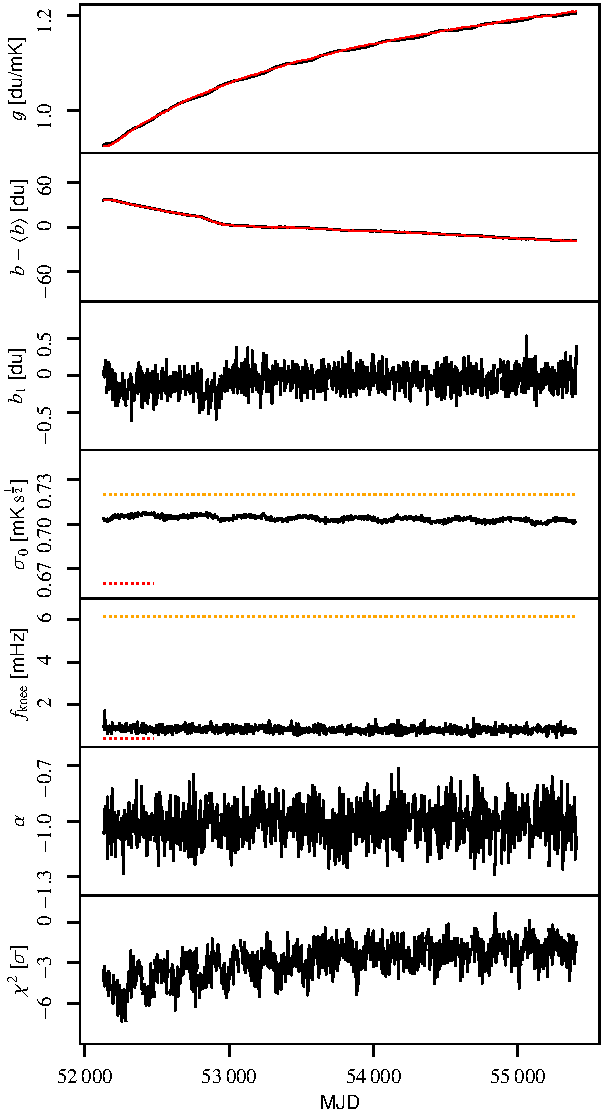
\includegraphics[width=\linewidth]{figures/instpar_CG_K113_v1.pdf}
	\caption{Overview of \K113. The red solid lines in first and second panel  are the regressed gain and baseline from \WMAPnine, while the black lines in all panels are samples from the \cosmoglobe\ Gibbs chain. The red dashed and yellow dashed lines are reported $\sigma_0$ and $f_\mathrm{knee}$ values from the first-year \WMAP\ data analysis and GSFC measurements, respectively.}
	\label{fig:inst_K113}
\end{figure}


\subsection{Trace plots and correlations}
\label{sec:traceplots}

%\lipsum[1]
To illustrate the dependence of the goodness-of-fit on the noise model,
we inspect the 50th TOD segment, corresponding to MJDs 52285.2--52290.6, as a
function of Gibbs iteration, in Fig.~\ref{fig:inst_K113_gibbs}. This is one of
the worst-fitting TOD segments of the entire mission, with a reduced relative
$\chi^2$ of $-7.5$, equivalent to $\chi^2/n=0.993$. The line plots demonstrate a strong correlation between the noise parameters and the $\chi^2$, while the gain itself is almost completely uncorrelated with the variations in the $\chi^2$. As $\sigma_0$ is not formally sampled in the Gibbs chain, it is weakly dependent on $f_\mathrm{knee}$ and $\alpha$, making it more likely that it is the driver of the correlations in this figure. 

\begin{figure}[t]
	\centering
	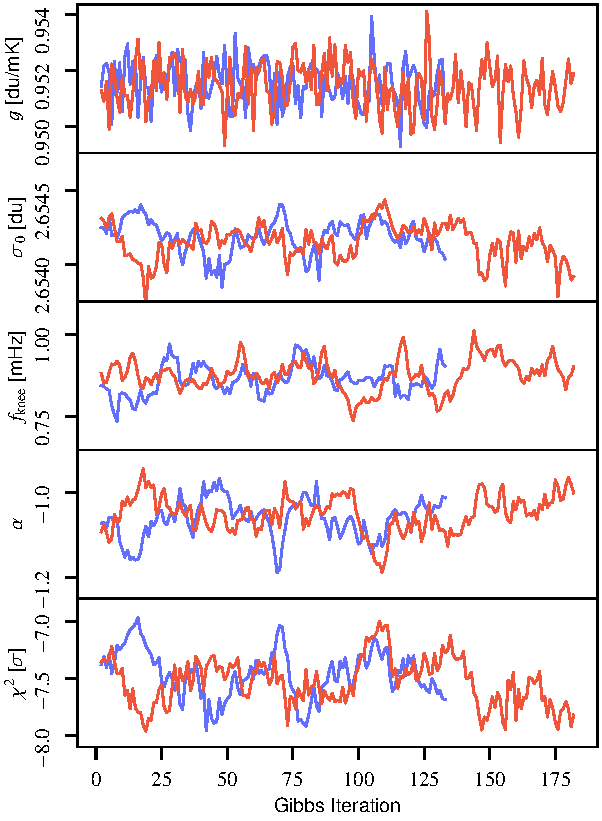
\includegraphics[width=\linewidth]{figures/instpar_CG_K113_samples_v1.pdf}
	\caption{Subset of \K113 Gibbs samples for both chains, arbitrarily colored red and blue. The parameters correspond to MJDs 52285.2--52290.6.}
	\label{fig:inst_K113_gibbs}
\end{figure}


%\subsection{Parameter correlations}
%\label{sec:correlations}

\begin{figure*}[t]
	\centering
	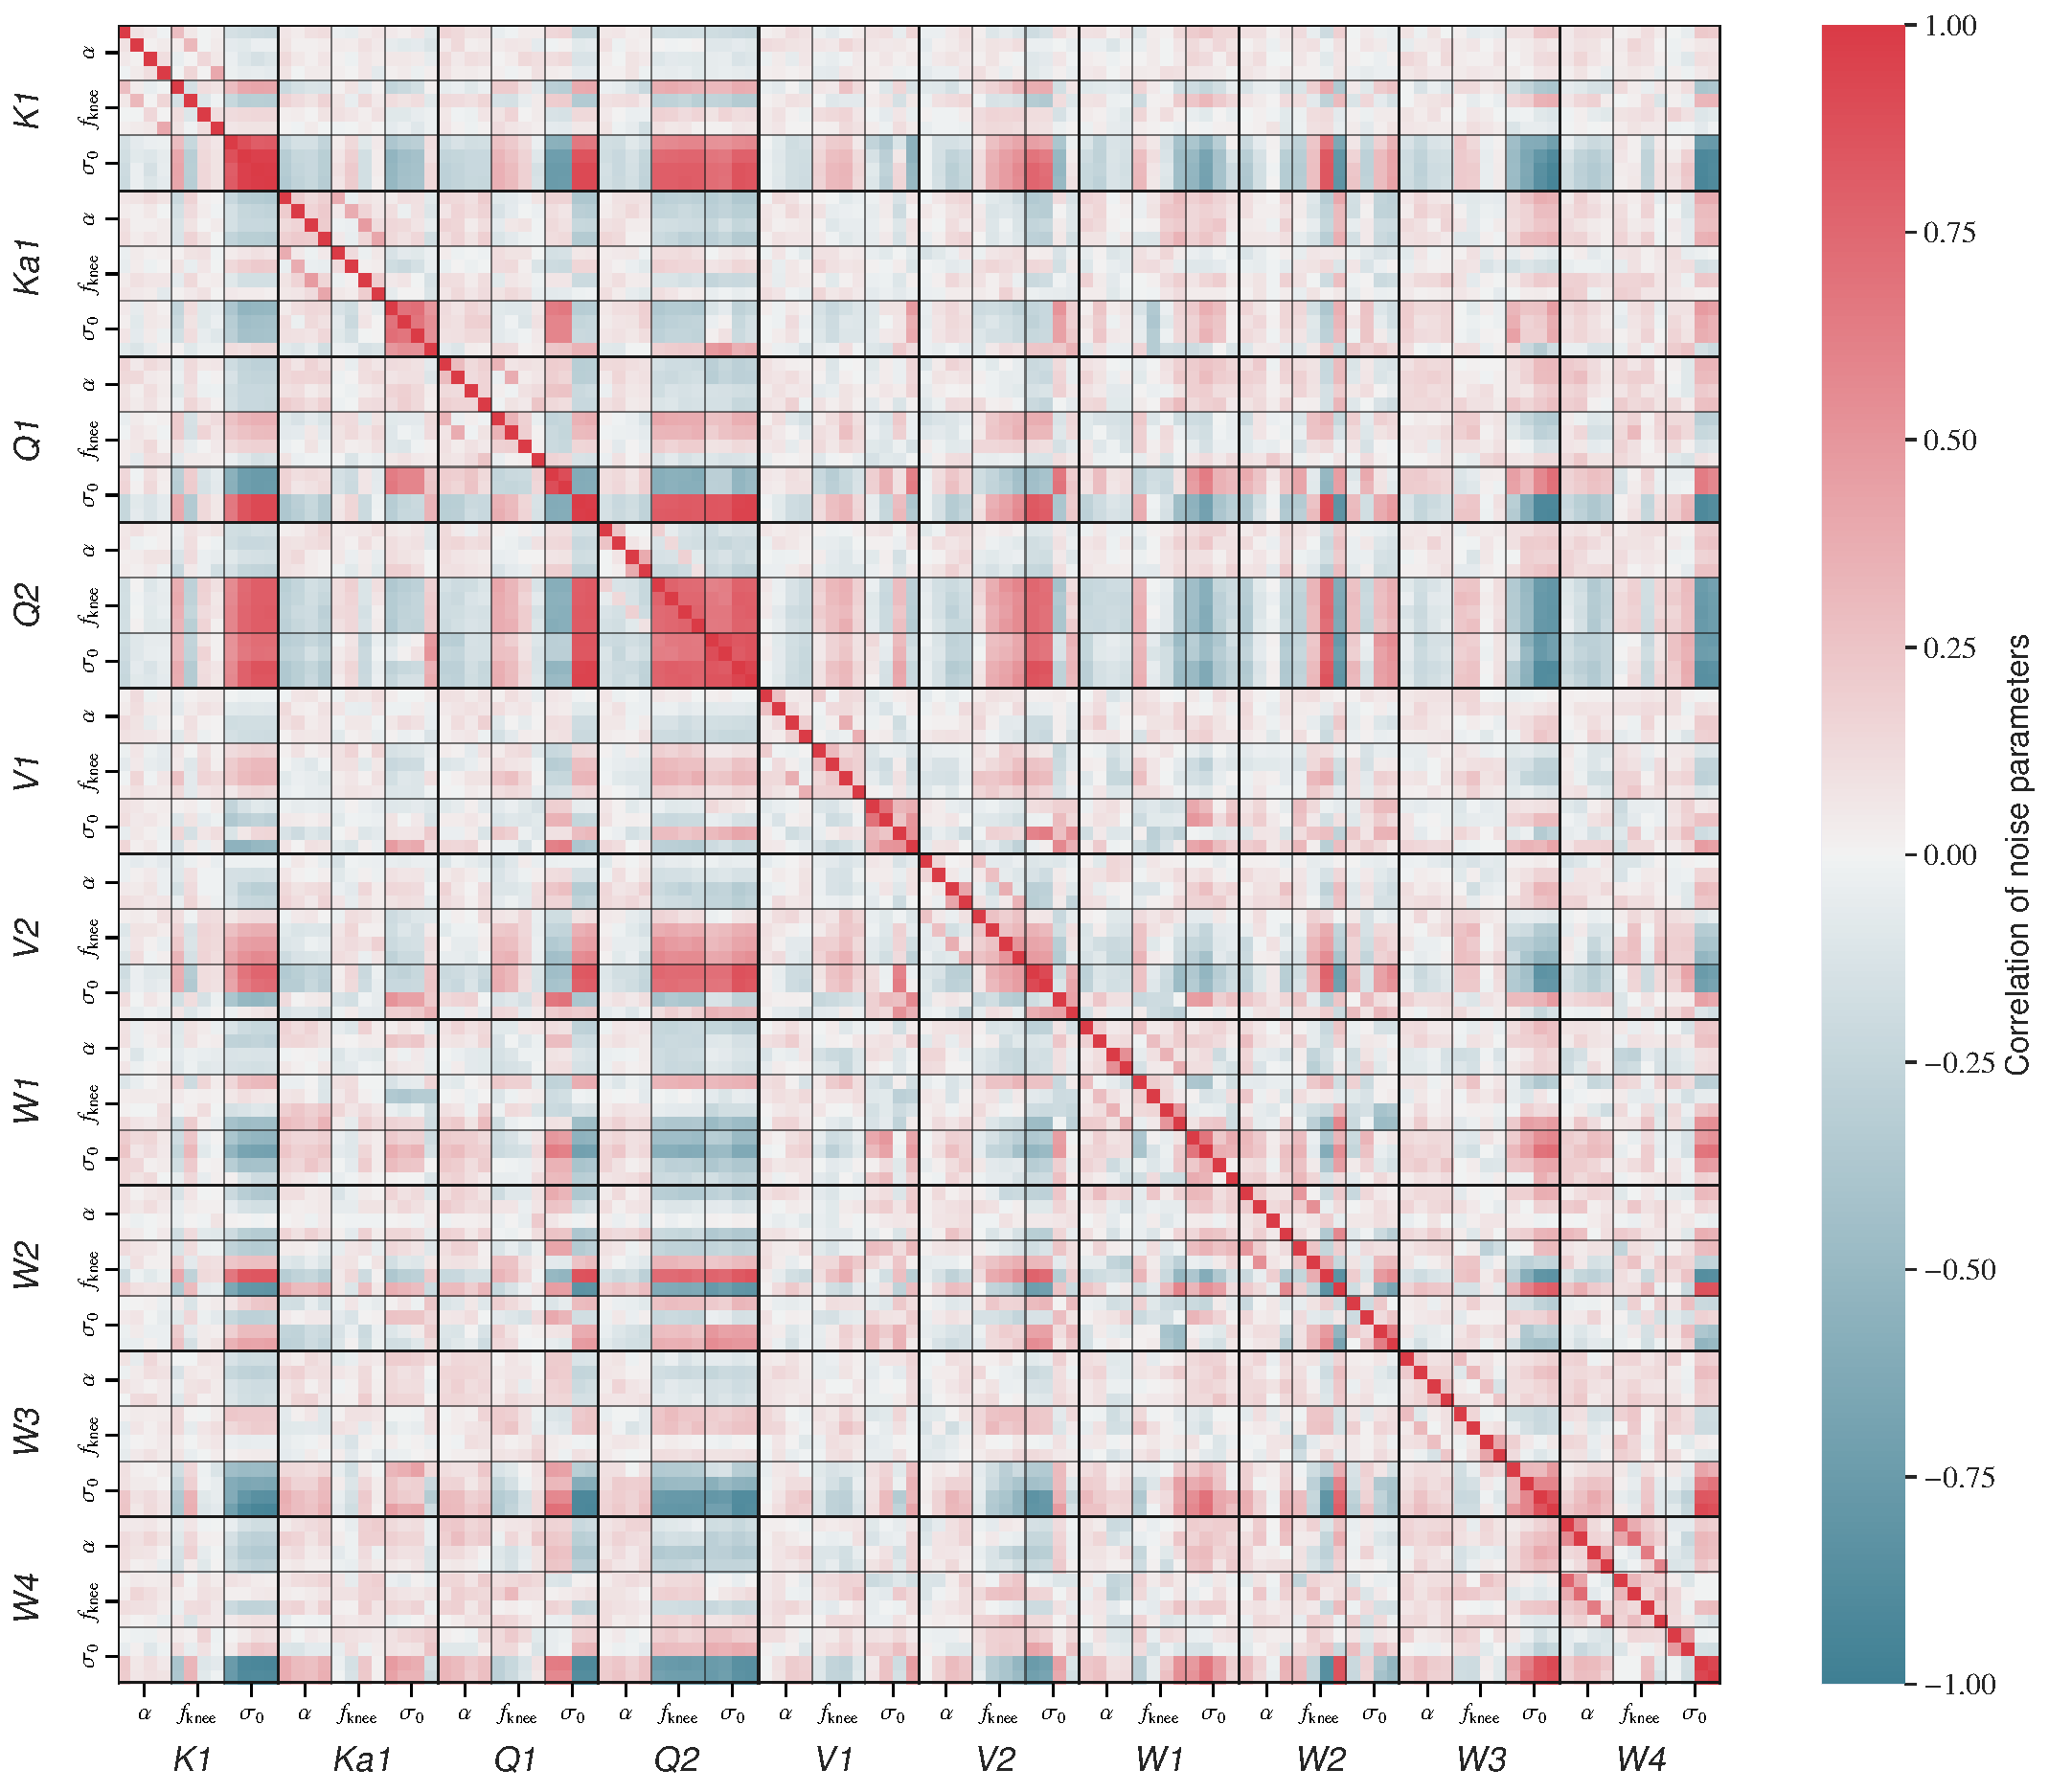
\includegraphics[width=\textwidth]{figures/noise_parameter_correlation.pdf}
	\caption{Noise parameter correlation matrix. We average over all Gibbs samples of the noise parameters $\xi^n=\{\alpha,f_\mathrm{knee},\sigma_0\}$ for each PID. We then find the correlation in time between these averages for the different bands and detector. The results here are for the calibrated white noise level, $\sigma_0[\mathrm{mK}]$. The values for each detector are ordered 13, 14, 23, and 24.}
	\label{fig:correlation}
\end{figure*}




\subsection{Gain and baselines}
\label{sec:gain}

\begin{figure}
	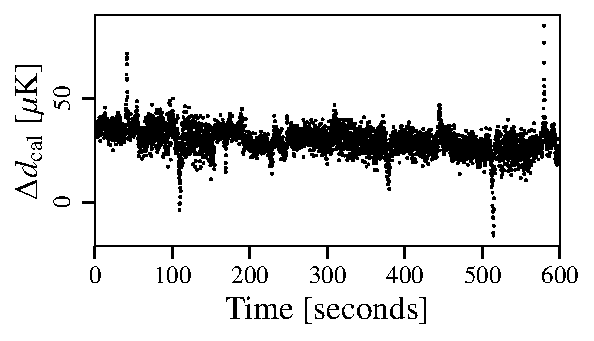
\includegraphics[width=\columnwidth]{figures/K113_TOD_diff_10min.pdf}
	\caption{Difference between the \cosmoglobe\ $\boldsymbol d_\mathrm{cal}=\boldsymbol d/g-\boldsymbol b - \boldsymbol s_\mathrm{sl}$ and the delivered calibrated TOD from \WMAP.}
	\label{fig:cal_comp_10min}
\end{figure}

\begin{figure}
	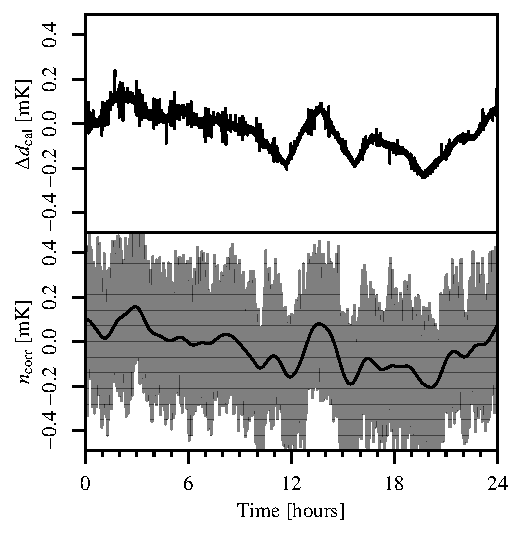
\includegraphics[width=\columnwidth]{figures/K113_TOD_diff_10hr.pdf}
	\caption{\textit{(top):} Difference between the \cosmoglobe\ $\boldsymbol d_\mathrm{cal}=\boldsymbol d/g-\boldsymbol b - \boldsymbol s_\mathrm{sl}$ and the delivered calibrated TOD from \WMAP. \textit{(Bottom):} Raw correlated noise (gray) and smoothed data with Gaussian kernel (black). This shows more clearly the hourly baseline subtraction from the \WMAP\ treatment.}
	\label{fig:cal_comp}
\end{figure}

To compare the calibrated TODs from \WMAP\ versus \cosmoglobe, it is  important to look at the \WMAP\ gain model,
\begin{equation}
	\label{eq:wmap_gain}
	g=\alpha\frac{\overline V-V_\circ-\beta(T_\mathrm{RXB}-290\,\mathrm K)}
	{T_\mathrm{FPA}-T_\circ}+(m\Delta t+c),
\end{equation}
where $\alpha$, $\V_\circ$, $\beta$, $T_\circ$, $m$, and $c$ are fit to a constant value across the mission for each radiometer. $\overline V$ represents the radio frequency bias powers per detector, and $T_\mathrm{RXB}$ and $T_\mathrm{FPA}$ are the receiver box and focal plane assembly temperatures, which are recorded every 23.04\,s. 
Evaluating the model as a function of $T_\mathrm{RXB}$ and $T_\mathrm{FPA}$ requires finding the housekeeping data for the thermistor that was physically closest to the relevant radiometer's focal plane on the satellite. As this requires detailed technical information about the specifications of the satellite's schematics layout that can easily be misunderstood, we do not attempt to reproduce the gain model given in Eq.~\eqref{eq:wmap_gain} in this work.
Although we are unable to reproduce the exact gain model parametrized in \citet{wmapexsupp}, the $23.04\,\mathrm s$ time dependence of the gain model on housekeeping data is a plausible explanation for the time-dependent noise variation in the different calibrated data solutions.

As reported in \citet{hinshaw2007}, the calibrated data archive has been calibrated using the procedure listed above, with a baseline subtracted each hour and the sidelobe subtracted. Figure~\ref{fig:cal_comp_10min} shows the \cosmoglobe\ timestream $\boldsymbol d/g-\boldsymbol s_\mathrm{sl}-\boldsymbol b$ with the \WMAP\ delivered calibrated signal subtracted. The most prominent feature is a $\sim25\,\mathrm{\mu K}$ offset, which is unsurprising, given the different treatment of baselines in our two pipelines. The second obvious difference is a series of spikes associated with Galactic plane crossings. The differences of order $50\,\mathrm{\mu K}$ correspond to sky brightness of order $10\,\mathrm{mK}$, equivalent to $\sim0.5\,\%$ deviations in the gain solution. This is twice as large as the 0.2\,\% uncertainty estimated in \citet{bennett2012} based on end-to-end simulations.

On longer timescales, as displayed in Figure~\ref{fig:cal_comp}, the most prominent feature is a varying signal of amplitude $0.2\,\mathrm{mK}$. This likely due to the hourly baseline subtraction mentioned above, which contrasts with the \cosmoglobe\ approach of assigning a linear baseline solution for the entire scan. The variations are commensurate with correlated noise, which for \K113 has ${f_\mathrm{knee}\sim0.5\,\mathrm{mHz}}$, corresponding to a little over half an hour. Therefore, the hourlong baseline subtraction essentially acts as a destriper, removing an estimate of the correlated noise. To test this hypothesis, we plot a realization of correlated noise generated by \commander, and find that the signals are very similar, both in amplitude and morphology.


We also compare the gain and baseline solutions throughout the course of the mission in Fig.~\ref{fig:inst_K113}. To recover the \WMAPnine\ gain solution, we directly compare the uncalibrated \WMAP\ data with the calibrated \WMAP\ data with a far sidelobe contribution convolved with the delivered \WMAPnine\ DA maps. We find that the calibrated and uncalibrated data can be related by
\begin{equation}
	d^\mathrm{raw}_t=g(d^\mathrm{cal}_t+s^\mathrm{sl}_t)+\sum_{i=0}^3c_i(t-t_0)^i,
\end{equation}
where the second term is a cubic polynomial with coefficients $c_i$ referenced to the time at the beginning of the scan $t_0$.
To calculate $s_t^\mathrm{sl}$, we convolve the \WMAP\ far sidelobes with \WMAPnine\ frequency maps with the Solar dipole from \citet{hinshaw2009} added back in.
We find that $d^\mathrm{raw}$ is consistent with the expression on the right at the level of $<0.1\,\mathrm{du}$ for all radiometers, suggesting that this estimate of $g$ and the baseline $c_0$ is a good approximation of the \WMAPnine\ calibration solution. An initial estimate using a linear baseline gave an unacceptably poor fit. Given that Eq.~(2) of \citet{jarosik2003a} employed a cubic baseline fit while fitting for transmission imbalance parameters, it is reasonable to assume that the official calibrated archive was created using a similar procedure.

The morphological characteristics of the \WMAPnine\ and \cosmoglobe\ gain solutions are similar, with a general trend to increase with time. Both solutions also follow a sinusoidal pattern, corresponding to temperature change due to L2's motion around the Sun \citep{wmapexsupp}. However, we do find the  \cosmoglobe\ \K-band gain has slightly more oscillatory features than the \WMAPnine\ solution. In general, the gains are consistent between \cosmoglobe\ and \WMAPnine\ within 1\,\%. For completeness, the full gain comparisons can be found in Fig.~\ref{fig:gain}. 



\subsection{Transmission imbalance}
\label{sec:xim}

The transmission imbalance parameters $x_\mathrm{im}$ are crucial to measure correctly because their misestimation can induce a large polarized signal that is coupled to the Solar dipole \citep{jarosik2007,bp17}. The uncertainty in $x_\mathrm{im}$ was quoted as the source of large-scale polarized features in the \WMAPnine\ maps, and a template of this effect was explicitly projected out in the pixel-space polarized covariance matrix. 

We find $x_\mathrm{im}$ values that are largely consistent with the values reported in \citet{bennett2012}, albeit with some outliers. We find in general that the 68\,\% confidence intervals from \cosmoglobe\ are smaller than the fiducial values, although we caution against a direct comparison of these values since such different procedures were used for estimating the uncertainties.

%\begin{figure}[t]
%	\centering
%	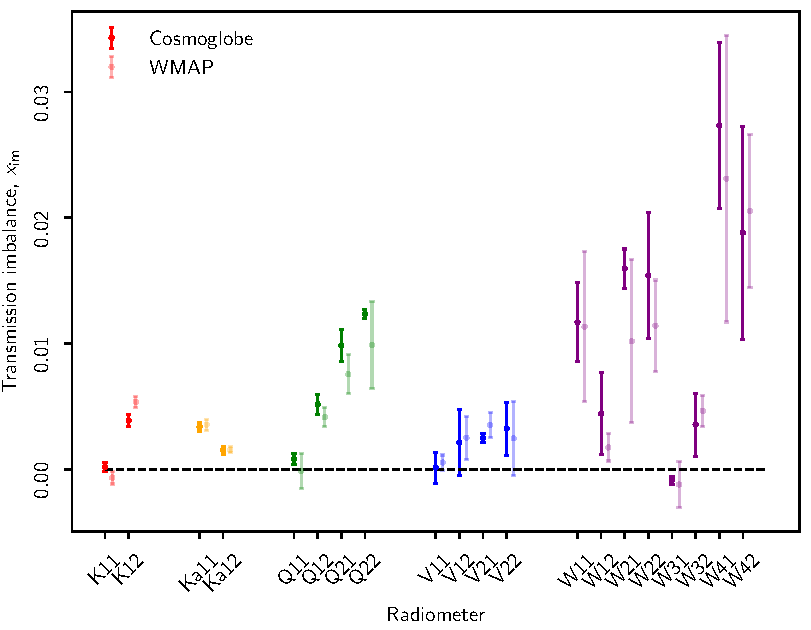
\includegraphics[width=\linewidth]{figures/x_im_CG_v1.pdf}
%	\caption{Transmission imbalance}
%	\label{fig:x_im}
%\end{figure}

%\begin{table}
%\newdimen\tblskip \tblskip=5pt
%\caption{Transmission imbalance parameters for each \WMAP\ radiometer as estimated in the current analysis (\emph{second column}) and in the official 9-year \WMAP\ analysis (\emph{third column}). Our uncertainties indicate $1\,\sigma$ marginal posterior standard deviations. }
%\label{tab:dipole}
%\vskip -8mm
%\footnotesize
%\setbox\tablebox=\vbox{
% \newdimen\digitwidth
% \setbox0=\hbox{\rm 0}
% \digitwidth=\wd0
% \catcode`*=\active
% \def*{\kern\digitwidth}
%%
%  \newdimen\dpwidth
%  \setbox0=\hbox{.}
%  \dpwidth=\wd0
%  \catcode`!=\active
%  \def!{\kern\dpwidth}
%%
%  \halign{\hbox to 1.8cm{#\leaderfil}\tabskip 2em&
%    \hfil$#$\hfil \tabskip 2em&
%    \hfil$#$\hfil \tabskip 0em\cr
%\noalign{\doubleline}
%\omit\hfil\sc Radiometer \hfil& x_{\mathrm{im}}^{\mathrm{CG}}& x_{\mathrm{im}}^{\mathrm{WMAP}}\cr
%\noalign{\vskip 3pt\hrule\vskip 5pt}
%K11 &   0.00018 \pm  0.00013  &  -0.00067 \pm  0.00017 \cr
%K12 &   0.00388 \pm  0.00015  &   0.00536 \pm  0.00014 \cr
%Ka11 &   0.00339 \pm  0.00012  &   0.00353 \pm  0.00017 \cr
%Ka12 &   0.00150 \pm  0.00010  &   0.00154 \pm  0.00008 \cr
%Q11 &   0.00081 \pm  0.00016  &  -0.00013 \pm  0.00046 \cr
%Q12 &   0.00517 \pm  0.00027  &   0.00414 \pm  0.00025 \cr
%Q21 &   0.00985 \pm  0.00042  &   0.00756 \pm  0.00052 \cr
%Q22 &   0.01235 \pm  0.00011  &   0.00986 \pm  0.00115 \cr
%V11 &   0.00012 \pm  0.00041  &   0.00053 \pm  0.00020 \cr
%V12 &   0.00212 \pm  0.00089  &   0.00250 \pm  0.00057 \cr
%V21 &   0.00246 \pm  0.00012  &   0.00352 \pm  0.00033 \cr
%V22 &   0.00323 \pm  0.00070  &   0.00245 \pm  0.00098 \cr
%W11 &   0.01169 \pm  0.00105  &   0.01134 \pm  0.00199 \cr
%W12 &   0.00442 \pm  0.00109  &   0.00173 \pm  0.00036 \cr
%W21 &   0.01595 \pm  0.00052  &   0.01017 \pm  0.00216 \cr
%W22 &   0.01540 \pm  0.00167  &   0.01142 \pm  0.00121 \cr
%W31 &  -0.00089 \pm  0.00010  &  -0.00122 \pm  0.00062 \cr
%W32 &   0.00354 \pm  0.00084  &   0.00463 \pm  0.00041 \cr
%W41 &   0.02734 \pm  0.00219  &   0.02311 \pm  0.00380 \cr
%W42 &   0.01882 \pm  0.00282  &   0.02054 \pm  0.00202 \cr
%\noalign{\vskip 5pt\hrule\vskip 5pt}}}
%\endPlancktablewide
%\end{table}




\subsection{Instrumental noise and goodness-of-fit}
\label{sec:noise}

\begin{table*}
\newdimen\tblskip \tblskip=5pt
\caption{Summary of noise properties. }
\label{tab:noise}
\vskip -4mm
\footnotesize
\setbox\tablebox=\vbox{
 \newdimen\digitwidth
 \setbox0=\hbox{\rm 0}
 \digitwidth=\wd0
 \catcode`*=\active
 \def*{\kern\digitwidth}
%
  \newdimen\dpwidth
  \setbox0=\hbox{.}
  \dpwidth=\wd0
  \catcode`!=\active
  \def!{\kern\dpwidth}
%
  \halign{\hbox to 2.cm{#\leaderfil}\tabskip 2em&
    \hfil#\hfil \tabskip 1em&
    \hfil$#$\hfil \tabskip 0.5em&
    \hfil$#$\hfil \tabskip 0.5em&
    \hfil$#$\hfil \tabskip 2em&    
    \hfil$#$\hfil \tabskip 0.5em&
    \hfil$#$\hfil \tabskip 0.5em&
    \hfil$#$\hfil \tabskip 2em&
    \hfil$#$\hfil \tabskip 0em\cr
\noalign{\doubleline}
\omit&&\multispan3\hfil Sensitivity, $\sigma_0$ (mK\,$\sqrt{\mathrm{s}}$) \hfil&
\multispan3\hfil Knee frequency, $f_{\mathrm{knee}}$ (mHz) \hfil& \cr
\noalign{\vskip -3pt}
\omit&&\multispan3\hrulefill&\multispan3\hrulefill&\omit\cr
\noalign{\vskip 3pt} 
Radiometer & Diode & \textrm{GSFC} & \textrm{WMAP} & \textrm{CG}/\sqrt{2} & \textrm{GSFC} & \textrm{WMAP} & \textrm{CG}/\sqrt{2} & \mathrm{Slope}, \alpha \cr
\noalign{\vskip 3pt\hrule\vskip 5pt}
K11  &  1  &  0.72  &  0.66  &   0.704 \pm  0.002  &  6.13  &  0.4  &    0.82 \pm   0.20  &   -1.01 \pm   0.10 \cr
\omit &  2  &  &  &   0.708 \pm  0.003  &  &  &    0.63 \pm   0.14  &   -0.95 \pm   0.10 \cr
K12  &  1  &  0.87  &  0.75  &   0.796 \pm  0.004  &  5.37  &  0.51  &    0.42 \pm   0.19  &   -0.93 \pm   0.12 \cr
\omit &  2  &  &  &   0.780 \pm  0.005  &  &  &    0.71 \pm   0.15  &   -1.02 \pm   0.10 \cr
Ka11  &  1  &  0.75  &  0.71  &   0.788 \pm  0.001  &  1.66  &  0.71  &    1.20 \pm   0.22  &   -1.02 \pm   0.09 \cr
\omit &  2  &  &  &   0.777 \pm  0.001  &  &  &    1.19 \pm   0.22  &   -1.02 \pm   0.09 \cr
Ka12  &  1  &  0.77  &  0.72  &   0.788 \pm  0.003  &  1.29  &  0.32  &    0.62 \pm   0.16  &   -0.99 \pm   0.11 \cr
\omit &  2  &  &  &   0.784 \pm  0.001  &  &  &    0.63 \pm   0.13  &   -1.01 \pm   0.11 \cr
Q11  &  1  &  0.99  &  0.92  &   0.998 \pm  0.002  &  3.21  &  1.09  &    1.06 \pm   0.16  &   -1.09 \pm   0.09 \cr
\omit &  2  &  &  &   0.992 \pm  0.002  &  &  &    1.06 \pm   0.16  &   -1.10 \pm   0.09 \cr
Q12  &  1  &  0.95  &  1.02  &   1.159 \pm  0.007  &  3.13  &  0.35  &    0.45 \pm   0.47  &   -0.98 \pm   0.11 \cr
\omit &  2  &  &  &   1.146 \pm  0.007  &  &  &    0.83 \pm   0.14  &   -1.00 \pm   0.09 \cr
Q21  &  1  &  0.89  &  0.85  &   0.908 \pm  0.002  &  1.92  &  5.76  &    2.88 \pm   0.37  &   -1.10 \pm   0.07 \cr
\omit &  2  &  &  &   0.906 \pm  0.002  &  &  &    3.22 \pm   0.56  &   -1.10 \pm   0.06 \cr
Q22  &  1  &  1.04  &  0.99  &   1.074 \pm  0.004  &  4.61  &  8.62  &    3.95 \pm   0.54  &   -1.11 \pm   0.06 \cr
\omit &  2  &  &  &   1.064 \pm  0.003  &  &  &    4.05 \pm   0.64  &   -1.11 \pm   0.06 \cr
V11  &  1  &  1.25  &  1.22  &   1.551 \pm  0.003  &  2.56  &  0.09  &    1.27 \pm   0.15  &   -0.90 \pm   0.06 \cr
\omit &  2  &  &  &   1.539 \pm  0.003  &  &  &    1.19 \pm   0.14  &   -0.89 \pm   0.06 \cr
V12  &  1  &  1.07  &  1.11  &   1.398 \pm  0.002  &  4.49  &  1.41  &    2.11 \pm   0.20  &   -0.97 \pm   0.05 \cr
\omit &  2  &  &  &   1.432 \pm  0.002  &  &  &    1.88 \pm   0.17  &   -0.96 \pm   0.05 \cr
V21  &  1  &  1.01  &  0.97  &   1.241 \pm  0.298  &  2.43  &  0.88  &    1.50 \pm   0.24  &   -0.95 \pm   0.07 \cr
\omit &  2  &  &  &   1.217 \pm  0.294  &  &  &    1.60 \pm   0.26  &   -0.97 \pm   0.06 \cr
V22  &  1  &  1.13  &  1.1  &   1.443 \pm  0.300  &  3.06  &  8.35  &    4.01 \pm   0.85  &   -1.00 \pm   0.08 \cr
\omit &  2  &  &  &   1.415 \pm  0.316  &  &  &    3.08 \pm   0.65  &   -1.01 \pm   0.08 \cr
W11  &  1  &  1.18  &  1.35  &   1.938 \pm  0.005  &  16.2  &  7.88  &    5.59 \pm   0.53  &   -0.94 \pm   0.05 \cr
\omit &  2  &  &  &   1.895 \pm  0.005  &  &  &    8.99 \pm   0.85  &   -0.95 \pm   0.04 \cr
W12  &  1  &  1.41  &  1.61  &   2.301 \pm  0.005  &  15.1  &  0.66  &    3.91 \pm   0.42  &   -0.89 \pm   0.05 \cr
\omit &  2  &  &  &   2.345 \pm  0.006  &  &  &    4.81 \pm   0.53  &   -0.89 \pm   0.05 \cr
W21  &  1  &  1.38  &  1.61  &   2.225 \pm  0.007  &  1.76  &  9.02  &   13.57 \pm   1.47  &   -0.89 \pm   0.03 \cr
\omit &  2  &  &  &   2.292 \pm  0.006  &  &  &    5.06 \pm   0.95  &   -0.93 \pm   0.05 \cr
W22  &  1  &  1.44  &  1.72  &   2.291 \pm  0.006  &  0.77  &  7.47  &    3.02 \pm   0.53  &   -0.98 \pm   0.05 \cr
\omit &  2  &  &  &   2.232 \pm  0.007  &  &  &    7.26 \pm   1.05  &   -0.95 \pm   0.04 \cr
W31  &  1  &  1.47  &  1.65  &   2.328 \pm  0.005  &  1.84  &  0.93  &    1.30 \pm   0.46  &   -0.99 \pm   0.07 \cr
\omit &  2  &  &  &   2.322 \pm  0.006  &  &  &    1.97 \pm   0.28  &   -0.98 \pm   0.06 \cr
W32  &  1  &  1.69  &  1.86  &   2.707 \pm  0.015  &  2.39  &  0.28  &    1.59 \pm   0.29  &   -0.98 \pm   0.07 \cr
\omit &  2  &  &  &   2.579 \pm  0.015  &  &  &    1.40 \pm   0.39  &   -1.00 \pm   0.07 \cr
W41  &  1  &  1.6  &  1.71  &   2.519 \pm  0.010  &  8.46  &  46.5  &   26.81 \pm   1.83  &   -0.92 \pm   0.04 \cr
\omit &  2  &  &  &   2.479 \pm  0.009  &  &  &   24.75 \pm   1.63  &   -0.92 \pm   0.04 \cr
W42  &  1  &  1.43  &  1.65  &   2.221 \pm  0.017  &  5.31  &  26.0  &   16.10 \pm   1.09  &   -0.94 \pm   0.04 \cr
\omit &  2  &  &  &   2.202 \pm  0.015  &  &  &   17.11 \pm   1.19  &   -0.94 \pm   0.04 \cr
\noalign{\vskip 5pt\hrule\vskip 5pt}}}
\endPlancktablewide
\end{table*}

The noise fitting, as outlined in Sect.~\ref{sec:algorithms}, inherently depends on the data being fit well by both the sky model and the instrument model. In practice, correlated noise fitting can model any unmodeled signals, so the power spectrum and TODs must be carefully scrutinized before any conclusions can be made about the corresponding maps.

The white noise level in raw du is not strictly sampled, but is estimated conditioned on the instrumental parameters and the sky parameters. However, the calibrated white noise level $\sigma_0[\mathrm K]=\sigma_0[\mathrm{du}]/g$ does depend on the gain quite directly, which allows us to test the effects of the calibration on the instrument senstivity itself. The calibrated white noise level follows a biannual trend indicative of a system temperature variation, which is to be expected given the radiometer equation
\begin{equation}
	\sigma_0[\mathrm V]\propto gT_\mathrm{sys}.
\end{equation}
Aside from an overall amplitude shift due to the absolute calibration variation, the shape of the white noise level is stable throughout the Gibbs chain.

The knee frequencies for each channel lie between the reported values in \citet{jarosik2003a} for both the Goddard Space Flight Center (GSFC) laboratory measurements and those from the first year of data collection. Nearly all radiometers have constant $f_\mathrm{knee}$ throughout the mission, with a few notable exceptions. First, all \W-band channels display some amount of temporal variation that does not seem to be associated with any sinusoidal features. Second, all \Q2 channels, \V223, and \V224 all display a similar asymptotic drift in time. We have not found any instrumental effects that share this feature.
The PSD slope $\alpha$ is around $-1$ for each radiometer, albeit with high scatter for the lower frequencies. As expected, the uncertainty in $\alpha$ decreases as $f_\mathrm{knee}$ increases, since there are more datapoints to fit below $f_\mathrm{knee}$ where the constraining power on $\alpha$ is the strongest.


The most striking feature of the reduced normalized $\chi^2$ is its amplitude
and its semiannual periodicity.  Given the noise model and data residual, we
can evaluate the goodness-of-fit in the form of the relative $\chi^2$. Here, we
find that approximately half of the radiometers have a $\chi^2$ value at least
$6\sigma$ above or below the expected value.  Given perfect Gaussian residuals,
we would expect the reduced sum of squares to be $n_\mathrm{tod}=2^N$ and be
within $\sqrt{2n_\mathrm{tod}}=2^{(N+1)/2}$ 68\,\% of the time. For a typical
\W-band scan of length $n_\mathrm{TOD}=2^{22}$, a $10\sigma$ model failure
corresponds to $\chi^2/n_\mathrm{TOD}=1.003$. Therefore, it is exceedingly
difficult to look at any given \WMAP\ scan in the time domain and identify a
model failure. In power spectrum space, i.e., in Fig.~\ref{fig:W413_psd}, the
data are still characterized well at all scales, despite this scan having a
$\chi^2$ that is $7\sigma$ above the expectation value. 




Only with aggressive smoothing, as in Fig.~\ref{fig:W413_psd_zoom}, does the
model failure become apparent at frequencies 1--10\,Hz.  Here, it is clear that
despite fitting the data well at the highest and lowest frequencies, it is in
the intermediate range of 1--5\,Hz where the $1/f$ model is a less accurate
fit to the residual power spectrum. Part of the cause of this failure is that the white
noise level is essentially fixed by the value of the power spectrum at the
Nyquist frequency, as it was computed by differencing adjacent samples. The
power spectrum has a downward trend beyond above 1\,Hz, indicating that the
data would be better fit by one or more terms proportional to $f^\alpha$. This
is phenomenologically similar to the \WMAP\ collaboration's approach of
describing the time-space autocorrelation as a cubic polynomial in $\log\Delta t$ \citep{jarosik2007}.  


In practice, the $1/f$ model has a small effect on the final data products, and
was not visible in noise models when we modeled the data in one day scans
rather than the longer 3--7 day scans due to the lower $n_\mathrm{TOD}$ giving
a higher uncertainty on the relative $\chi^2$.  Therefore, although this
strictly constitutes a deficiency in the model, it is in practice too small to
affect the results of the rest of the chain. The downturn of the noise PSD at
high frequencies is also present in, e.g., the \Planck\ HFI data
\citep[Fig.~1]{planck2014-a10}, so improved modeling of this form will be a
necessity in future \cosmoglobe\ endeavors, and will be used to improve the
\WMAP\ data processing.

\begin{figure}
	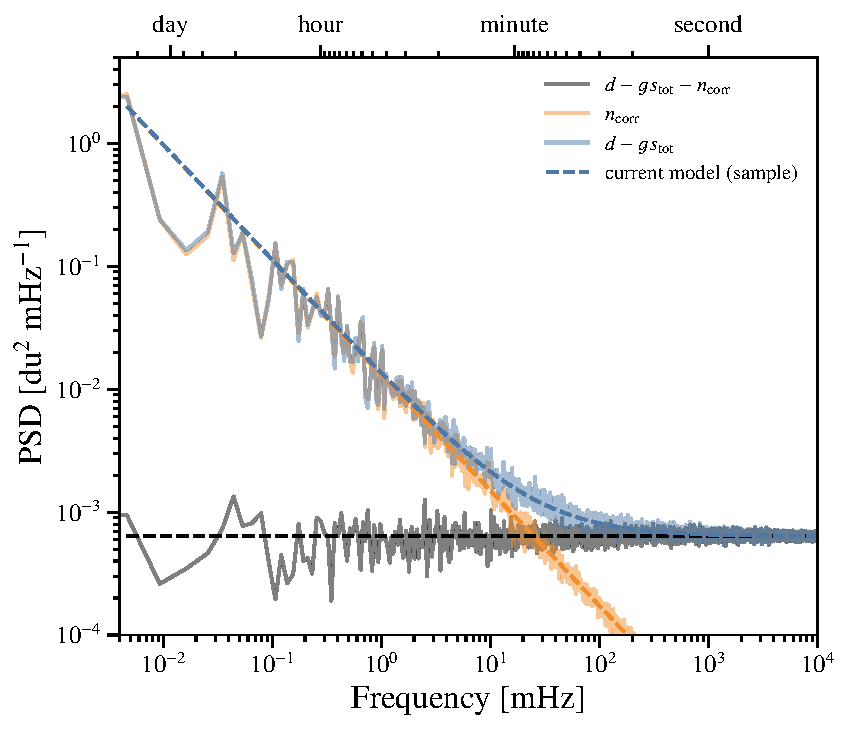
\includegraphics[width=\columnwidth]{figures/ps_test_W4_det1.pdf}
	\caption{PSD for radiometer \W413 that spans MJDs 52252.3--52254.8. The power spectrum of the blue line corresponds to the residual, while the gray line is the residual with a correlated noise realization removed.}
	\label{fig:W413_psd}
\end{figure}

\begin{figure}
	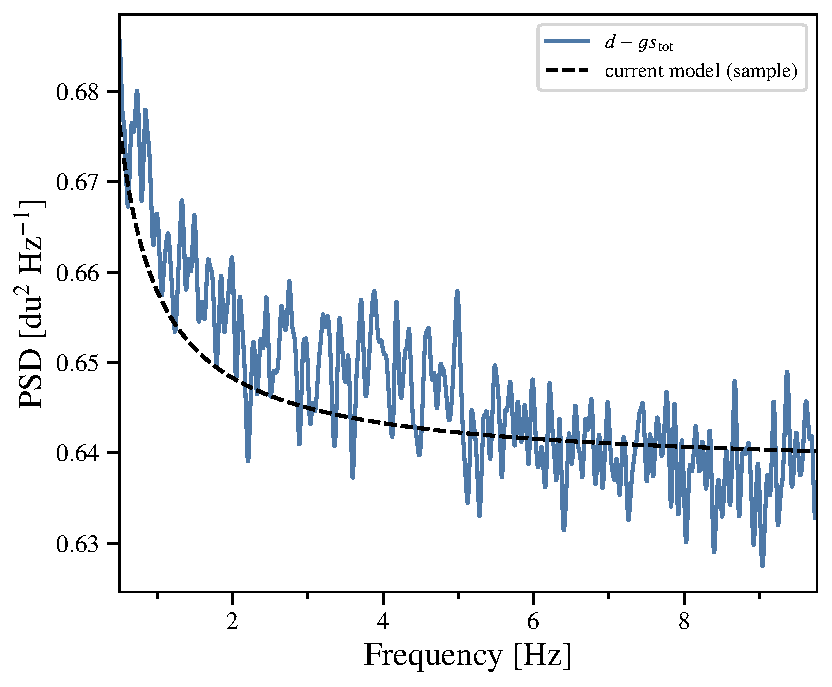
\includegraphics[width=\columnwidth]{figures/ps_test_W4_det1_zoom.pdf}
	\caption{PSD for radiometer \W413 that spans MJDs 52252.3--52254.8. 
	The black dashed line is a sample of the theoretical PSD, while the blue line is the smoothed residual power spectrum.
	}
	\label{fig:W413_psd_zoom}
\end{figure}





%\subsection{Frequency difference maps}




%Need to have the things that go directly into likelihood, the template-corrected WMAP data, theirs versus ours.
%
%Show the low-resolution one. Plotting the W3-W4, W1-W2, V1-V2, Q1-Q2, Ka-0.32K.
%Include the SED from the 03 paper, reference it, remove the power law.


%\lipsum[1-8]


%\subsection{Internal half-difference maps}

%\subsection{Comparison of noise rms maps}

%\begin{figure}
%	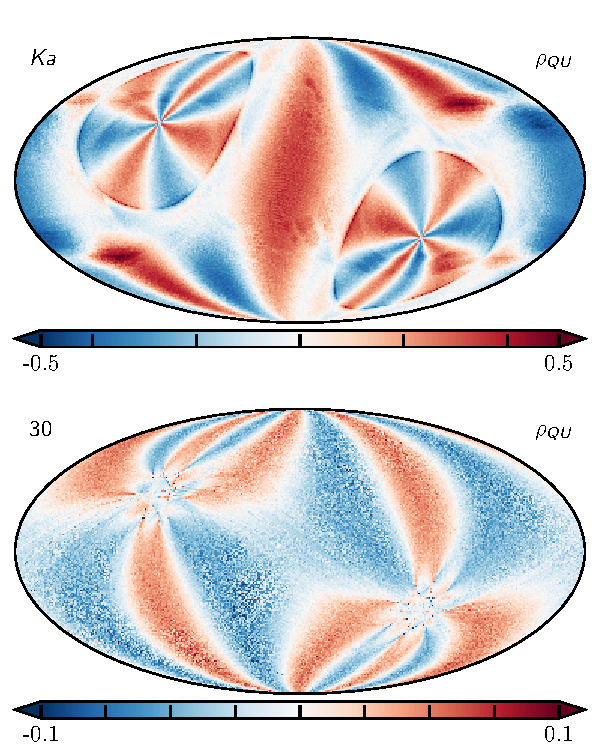
\includegraphics[width=\columnwidth]{figures/rho_QU.pdf}
%	\caption{$QU$ correlation for \WMAP\ \Ka-band \textit{(top)} and \Planck\ 30\,GHz \textit{(bottom)}. Note the differing dynamic range in the two maps.}
%	\label{fig:rho_qu}
%\end{figure}

%\subsection{Angular power spectra}



%\clearpage

%\section{High-level posterior distributions}
%\label{sec:maps}

%\subsection{Astrophysical sky model}
%\label{sec:skymodel}
%
%Given the frequency maps,\footnote{As the maps are deterministic functions of the instrumental parameters, they are discussed in Sect.~\ref{sec:maps}.} we can determine the component's amplitude maps as part of the Gibbs chain. Due to the high signal-to-noise of the \K-band map, which was not used in the \citet{bp01} for this reason, the spectral indices were not fit in this chain but rather drawn from prior distributions.








%\lipsum[5]


%\begin{figure}
%	\centering
%	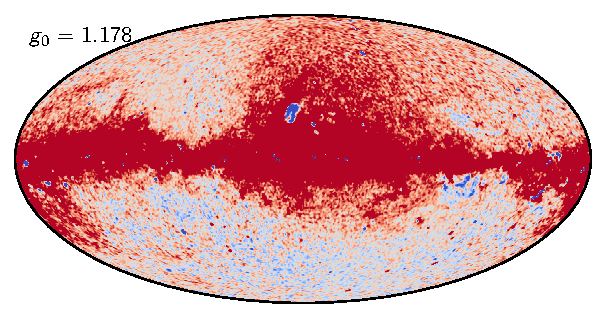
\includegraphics[width=\columnwidth]{figures/ame_g01_178.pdf}
%	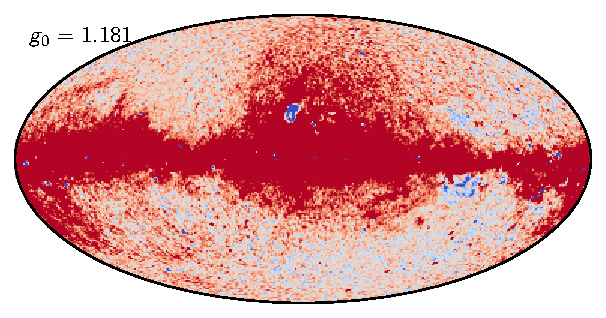
\includegraphics[width=\columnwidth]{figures/ame_g01_181.pdf}
%	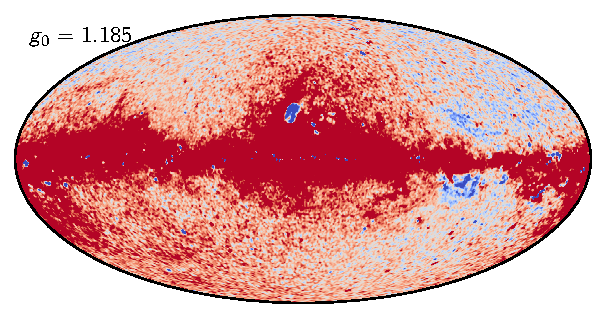
\includegraphics[width=\columnwidth]{figures/ame_g01_185.pdf}
%	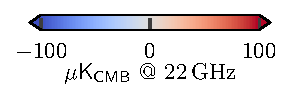
\includegraphics[width=0.5\columnwidth]{figures/cbar_100uK.pdf}
%	\caption{Dependence on AME amplitude evaluated at 22\,GHz as a function of absolute calibration. Each map comes from the fifth iteration of a dedicated \commander\ run that fixed $g_0$ while letting all other TOD parameters be fit. The values of $g_0=1.178$ and $g_0=1.185$ represent $3.5\sigma$ draws from the prior distribution with mean $1.1815$ and standard deviation $0.001$. The dipole visible in the top and bottom panels is aligned perfectly with the Solar dipole, and is directly due to variations in the \K-band absolute calibration.}
%	\label{fig:g0_ame}
%\end{figure}




%These parameters are themselves sampled conditioned on a full sky model.
%
%Remember that the frequency maps themselves are deterministic functions of the low-level sampled parameters.


%\subsection{Gain and baselines}

%\lipsum[1]



%\subsection{Transmission imbalance}



%\subsection{Noise characterization}

% \textit{The second main deviation\ldots} is in the treatment the noise power spectra. As shown
% in Sect~2.5 of \citet{jarosik2007}, the noise autocorrelation spectrum is fit
% on a year-by-year basis to a polynomial in $\log(\Delta t)$, where $\Delta t$
% is the time lag between data points. This method is very similar to the
% \commanderthree\ approach, which fits for the power spectrum in Fourier space
% using a correlated noise model of the form
% $\sigma_0^2(f/f_\mathrm{knee})^{\alpha}$. Properly parameterized, these two
% approaches should yield similar results, albeit with different levels of
% uncertainty and time resolution. However, we have confirmed that in many cases
% the simple $1/f$ noise model does not fit the signal-subtracted TOD, yielding
% $\chi^2$ values that are up to $10\sigma$ discrepant from their expected
% values.  [Show, discuss figure with the PSDs, residual spectrum, and Bessel
% filter.]
% 
% Deviations from the $1/f$ model consist either of a linear increase or downturn
% above 10\,Hz. This can be partially explained by the use of a two pole Bessel
% low-pass filter just prior to signal quantization, which introduces a 2.62\%
% correlation between 25.6\,ms sample integrations
% \citep[][Sect.~5.3]{jarosik2003:MAP}. The exact form of the Bessel filter was
% not used on flight data, but rather the parametric fit as discussed above.
% However, the filter is designed to reduce the signal by half at 100\,Hz, and as
% such has a negligible effect. 




%\subsection{Goodness-of-fit}

%\lipsum[1-4]

%\clearpage


\section{Frequency maps}
\label{sec:maps}

In this section, we present the reprocessed \WMAP\ frequency maps and their properties. In Sect~\ref{ssec:means} we present the reprocessed \WMAP\ maps themselves, commenting on notable features. Section~\ref{sec:wmap_comparison} compares the properties of the individual DAs with the published \WMAPnine\ results, while Sect.~\ref{sec:internal_consistency} focuses on the internal consistency between the \WMAP\ channels themselves. Finally, we assess the consistency between the LFI channels and \WMAP\ in Sect.~\ref{sec:lfi_consistency} and compare with legacy results.



\subsection{Map summary statistics}
\label{ssec:means}

For each DA, we present the mean maps, the white noise contribution in the form of RMS maps, and the standard deviation of the maps accounting for the sampling of instrumental parameters. Each mean map retains the Solar dipole, which we will estimate separately in Sect.~\ref{sec:dipole}. Additionally, we present inverse-weighted mean maps of \Q, \V, and \W\ rather than displaying each individual DA.

The \K-band, \Ka-band, \Q-band, \V-band, and \W-band mean maps are presented in Figs.~\ref{fig:kband}, \ref{fig:kaband}, \ref{fig:qband}, \ref{fig:vband}, and \ref{fig:wband}, respectively, given in $\mu\mathrm{K_{CMB}}$ units. 
The \Q, \V, and \W-band maps are generated by inverse-variance weighting the individual DAs.
The temperature maps are presented at full resolution, while the polarization maps have been smoothed with a $2^\circ$ Gaussian beam. The maps in temperature behave as expected, with consistent Solar dipole and Galactic foreground emission decreasing as the frequency increases. Similarly, the polarized maps decrease from \K--\V-band following the expected synchrotron behavior, with a slight increase at \W-band due to the contribution of thermal dust. Most striking, especially when compared with the delivered \WMAPnine\ maps, is the lack of transmission imbalance modes or poorly measured modes in the polarized maps.

The RMS maps are computed during the mapmaking routine, adding $\sigma_{0,i}^{-2}$ for every timestep that horn is in a given pixel, appropriately scaled by polarization angle and imbalance parameters. The top row of Fig.~\ref{fig:K_rms_std} shows the white noise for the Stokes parameters and the correlation coefficient between Stokes $Q$ and $U$. The white noise pattern for $T$ follows the usual pattern with highest sensitivity at the North and South ecliptic poles, as well as circles around the poles corresponding to times when the partner horn is observing the opposite ecliptic pole. There are also regions of higher noise level corresponding to planets crossing the ecliptic, and regions of higher emission $\simeq140^\circ$ away from the Galactic center, which correspond to the times when the partner horn lies within the processing mask.

The polarized RMS maps share all of these characteristics, but with an overall amplitude shift due to polarization measurements having half the effective number of observations per pixel. In addition, the poles have a characteristic ``X''-like structure that is rotated $45^\circ$ degrees between $Q$ and $U$, corresponding to different polarization orientations. There are also characteristic large scale structures visible in Galactic coordinates, corresponding to polarization modes poorly constrained by the \WMAP\ scan strategy.

While the maps in the top row of Fig.~\ref{fig:K_rms_std} are directly comparable to the \WMAPnine\ products, the bottom row shows a unique product, the standard deviation and $QU$ correlation of the output chain maps. These maps can be considered the ``systematic'' error contributions, as their variation depends on the sampled instrumental parameters, i.e., gain, imbalance parameters, correlated noise, and sidelobe correction. The temperature map contains a clear quadrupole signature. This is due to the variation in the absolute calibration $g_0$, which changes the Solar dipole in the final map. In addition to the quadrupole, the Galactic plane also varies due to the gain solution being varied. As expected, the white noise patterns associated with the scan strategy also appear in the polarization maps, and become more clear in the temperature maps for the higher frequency DAs (Fig.~\ref{fig:std}).
As these maps only include 490 total samples out of full 500-sample Gibbs chain, they will be superseded by a larger future chain. While the quantitative solution will change, it is unlikely that the final maps will differ qualitatively from those presented here.


An additional useful term to consider is the difference between two arbitrary samples, which we show in Fig.~\ref{fig:Ksampdiff}. In temperature, the most clear term is a dipole corresponding to the absolute gain difference and the Galactic plane. There are also additional small lines associated with the scanning strategy, which correspond to different correlated noise realizations. In polarization, correlated noise is the dominant difference between two samples, with a small imprint of the Galactic plane due to relative gain variation. The polarization differences are aligned with \WMAP's scans, modulated by the polarization angle.

We also consider the spatial structure of the TOD corrections in pixel space, as shown in Fig.~\ref{fig:tod_corrections}. This corresponds to the TOD objects in Fig.~\ref{fig:timestreams} binned into Stokes $I$, $Q$, and $U$ maps. Note that the dynamic range of each of these figures varies by two orders of magnitude, indicating that some components most be subtracted more carefully than others. However, the amplitude of the signal is not proportional to the level of scrutiny necessary, as some, such as orbital dipole, are much more precisely known than the others. 

The variation of these TOD corrections is more important than the absolute amplitude. As shown in Fig.~\ref{fig:corrmap_stddev}, white noise is the dominant effect for $\ell\gtrsim100$ for all frequencies. For temperature, the low-multipole variation in the orbital dipole signal and far sidelobe corrections are the largest source of fluctuations and low multipoles, but remain orders of magnitude below the average signal. These fluctuations are directly related to absolute calibration uncertainty, and provide a practical limit to the magnitude gain effects the temperature signal. For the $C_\ell^\mathrm{EE}$ and $C_\ell^\mathrm{BB}$ spectra, the relative amplitude of the fluctuations are band-dependent. For example, bandpass leakage and orbital dipole corrections are the dominant effect, while for \Q-band, the correlated noise realizations contribute the most variation. In general, we find that for large angular scale polarization, modelling uncertainties in the form of gain and sidelobe estimation have a comparable effect to white noise and correlated noise estimates.



%\textit{Draft text} We can remove all of the expected signals in TOD space and bin $\boldsymbol r=(\data-\boldsymbol n_\mathrm{corr})/g-\boldsymbol s_\mathrm{tot}$, if the model is perfect we should get a map that is dominated by white noise. See Fig.~\ref{fig:Kres}.

\begin{figure*}
	\centering
	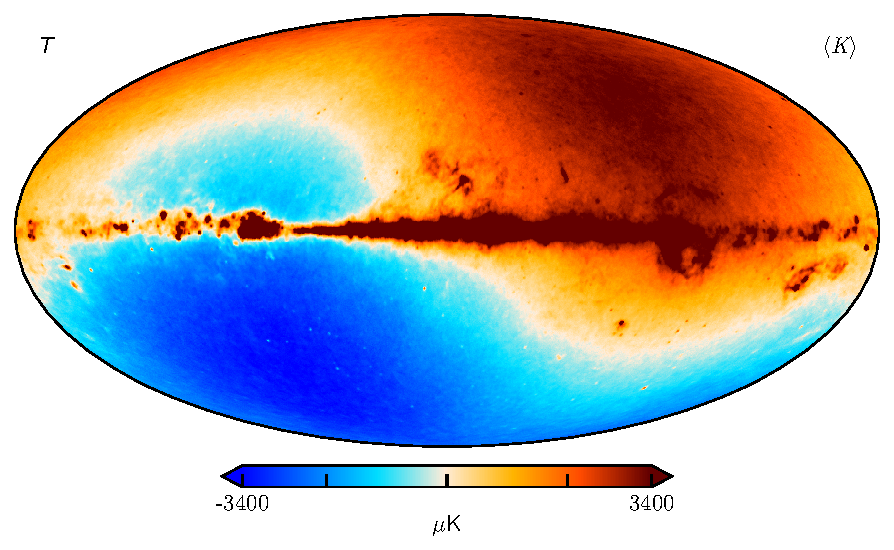
\includegraphics[width=0.75\textwidth]{figures/023-WMAP_K_mu_I.pdf}
	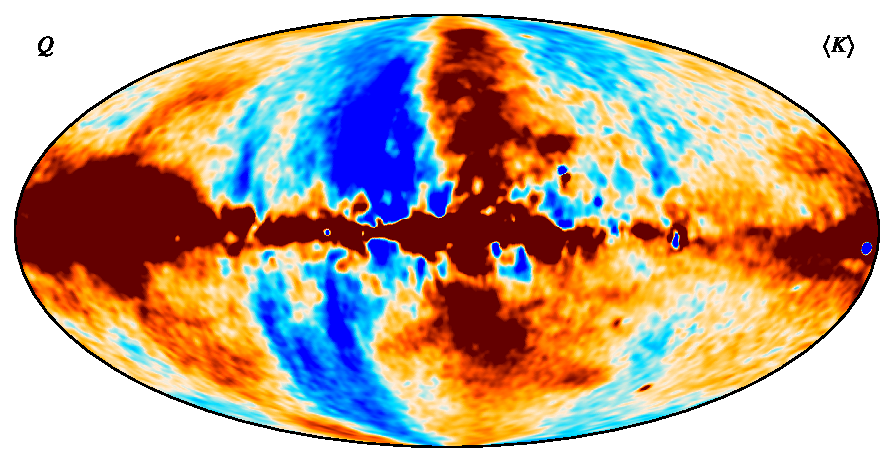
\includegraphics[width=0.75\textwidth]{figures/023-WMAP_K_mu_Q.pdf}
	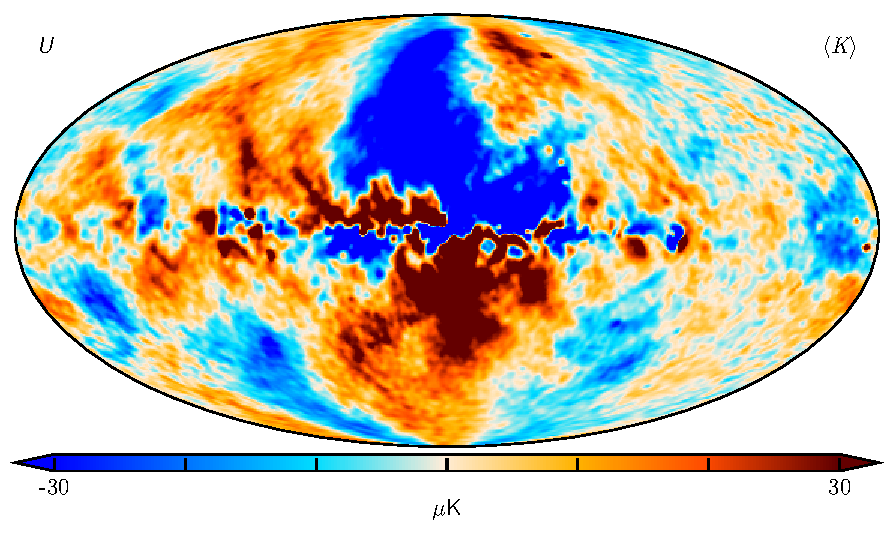
\includegraphics[width=0.75\textwidth]{figures/023-WMAP_K_mu_U.pdf}
	\caption{\K-band}
	\label{fig:kband}
\end{figure*}
\begin{figure*}
	\centering
	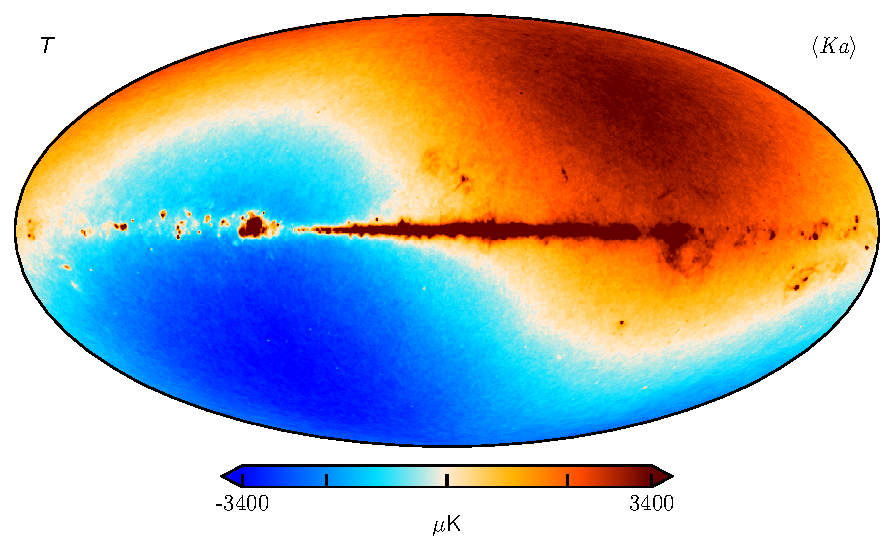
\includegraphics[width=0.75\textwidth]{figures/030-WMAP_Ka_mu_I.pdf}
	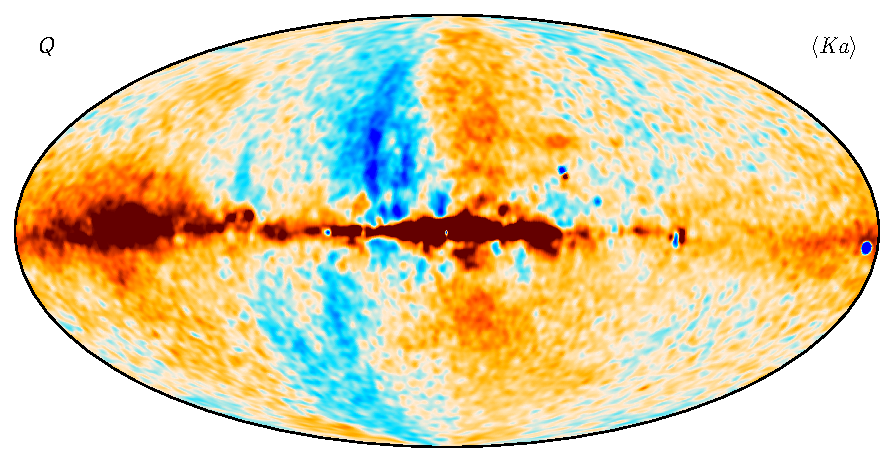
\includegraphics[width=0.75\textwidth]{figures/030-WMAP_Ka_mu_Q.pdf}
	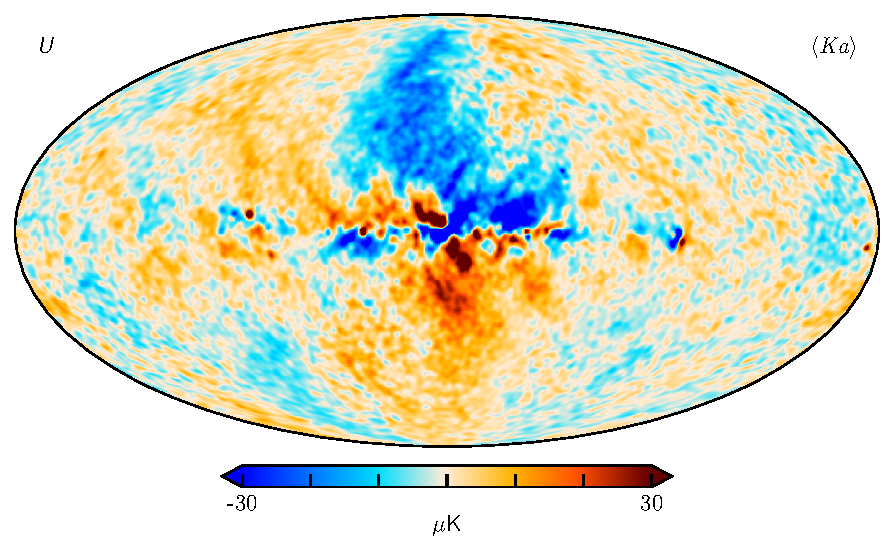
\includegraphics[width=0.75\textwidth]{figures/030-WMAP_Ka_mu_U.pdf}
	\caption{\Ka-band}
	\label{fig:kaband}
\end{figure*}
\begin{figure*}
	\centering
	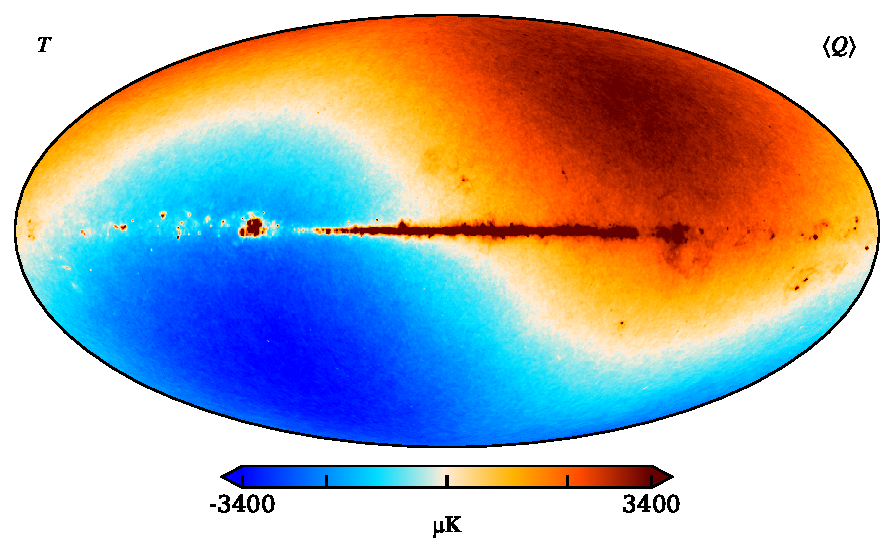
\includegraphics[width=0.75\textwidth]{figures/Q_mu_I.pdf}
	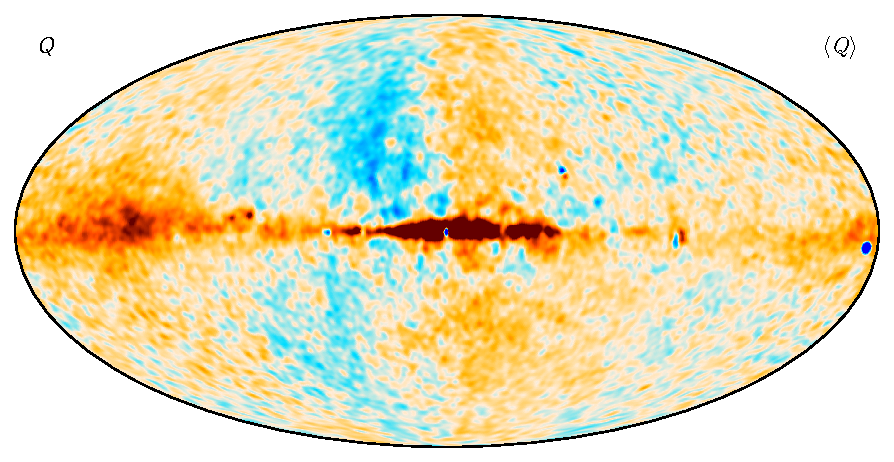
\includegraphics[width=0.75\textwidth]{figures/Q_mu_Q.pdf}
	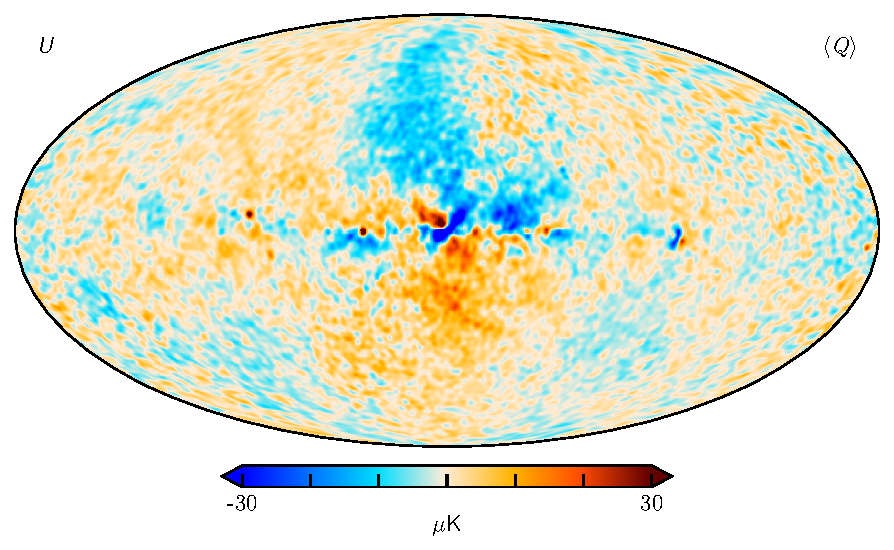
\includegraphics[width=0.75\textwidth]{figures/Q_mu_U.pdf}
	\caption{\Q-band}
	\label{fig:qband}
\end{figure*}
\begin{figure*}
	\centering
	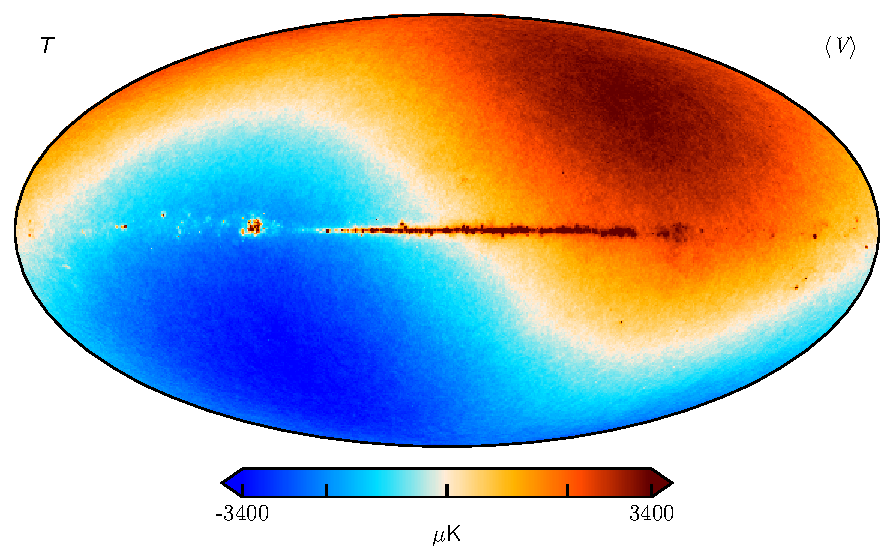
\includegraphics[width=0.75\textwidth]{figures/V_mu_I.pdf}
	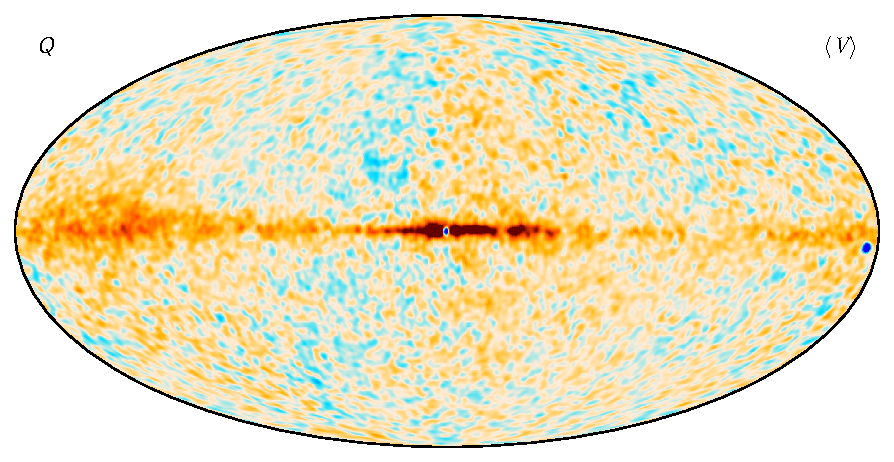
\includegraphics[width=0.75\textwidth]{figures/V_mu_Q.pdf}
	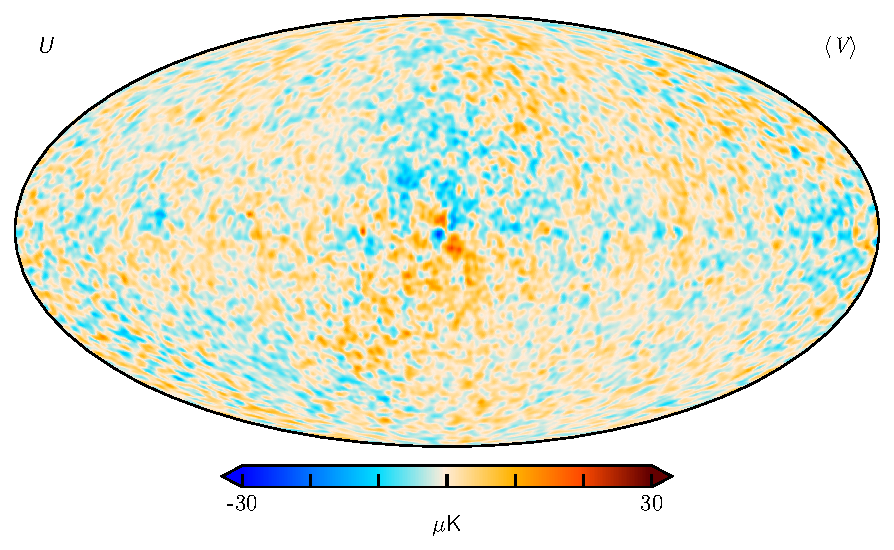
\includegraphics[width=0.75\textwidth]{figures/V_mu_U.pdf}
	\caption{\V-band}
	\label{fig:vband}
\end{figure*}
\begin{figure*}
	\centering
	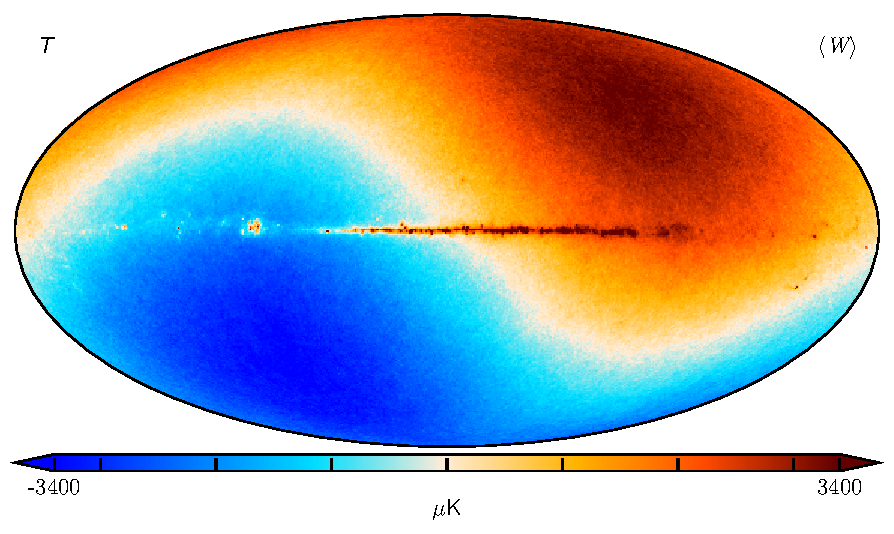
\includegraphics[width=0.75\textwidth]{figures/W_mu_I.pdf}
	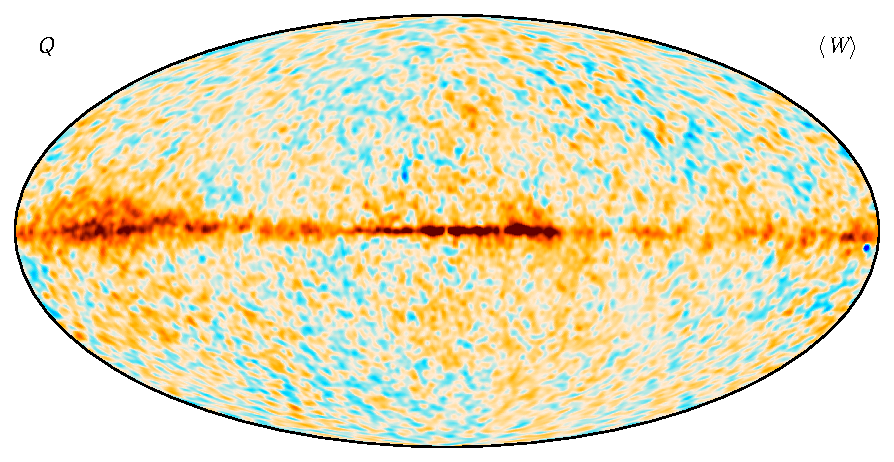
\includegraphics[width=0.75\textwidth]{figures/W_mu_Q.pdf}
	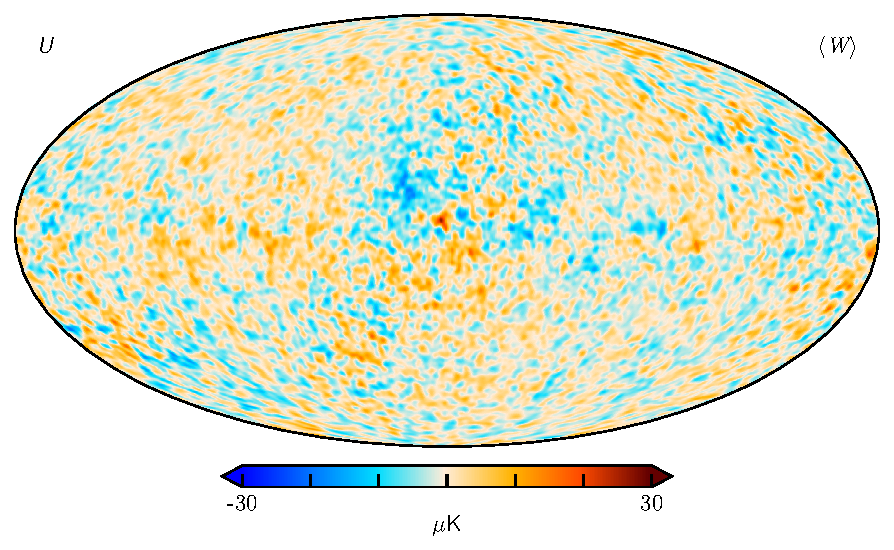
\includegraphics[width=0.75\textwidth]{figures/W_mu_U.pdf}
	\caption{\W-band}
	\label{fig:wband}
\end{figure*}


%\subsection{Posterior uncertainties}

\begin{figure*}[t]
	\centering
	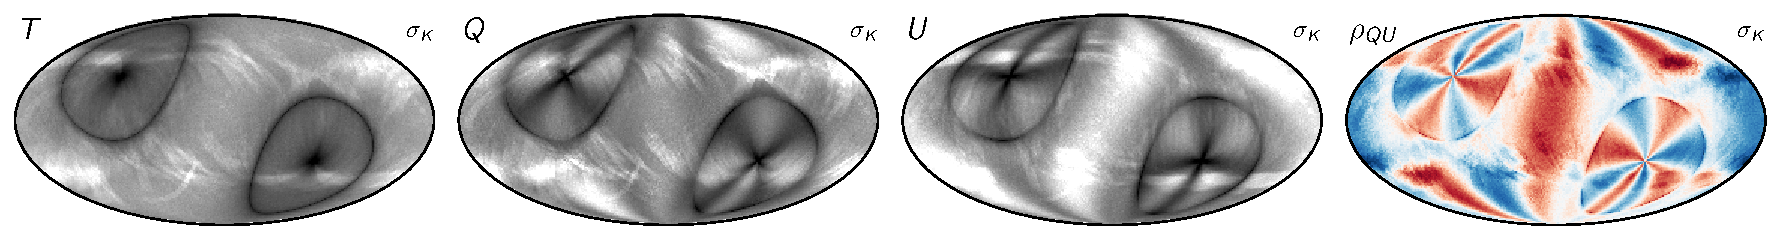
\includegraphics[width=\textwidth]{figures/023-WMAP_K_rms.pdf}\\
	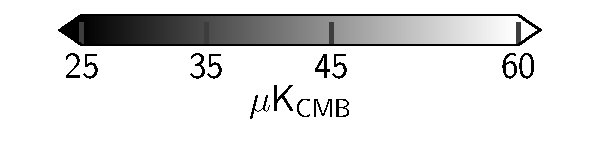
\includegraphics[width=0.245\textwidth]{figures/cbar_rms_I.pdf}
	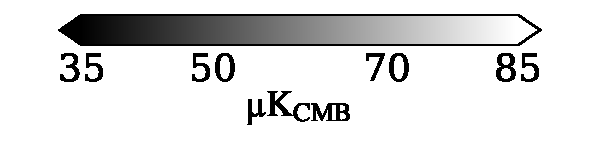
\includegraphics[width=0.245\textwidth]{figures/cbar_rms_P.pdf}
	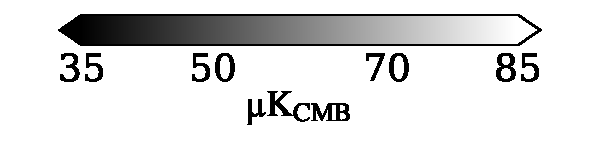
\includegraphics[width=0.245\textwidth]{figures/cbar_rms_P.pdf}
	\includegraphics[width=0.245\textwidth]{figures/cbar_rho.pdf}\\
	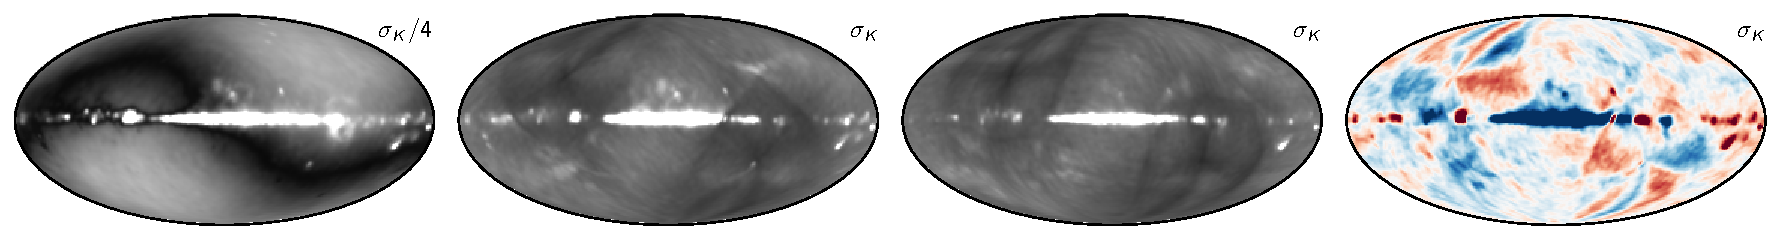
\includegraphics[width=\textwidth]{figures/023-WMAP_K_std.pdf}\\
	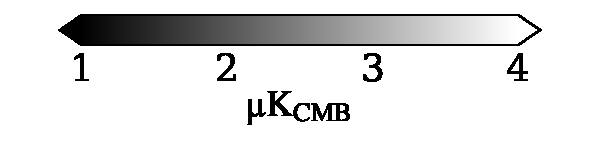
\includegraphics[width=0.245\textwidth]{figures/cbar_std.pdf}
	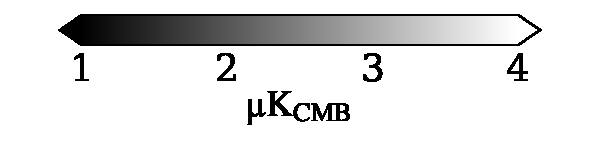
\includegraphics[width=0.245\textwidth]{figures/cbar_std.pdf}
	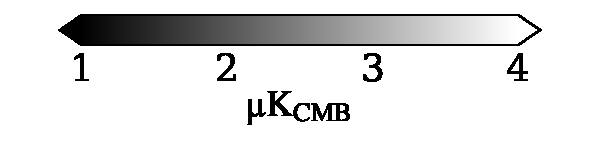
\includegraphics[width=0.245\textwidth]{figures/cbar_std.pdf}
	\includegraphics[width=0.245\textwidth]{figures/cbar_rho.pdf}\\
	\caption{Posterior variation maps for \K-band. Columns show the Stokes parameters and the correlation coefficient between $Q$ and $U$, while the rows show \textit{(top)} the white noise rms per pixel and \textit{(bottom)} the posterior standard deviation. The rms maps are unsmoothed, while the standard deviations have been smoothed to $7^\circ$.}
        \label{fig:K_rms_std}
\end{figure*}

\begin{figure*}[t]
	\centering
	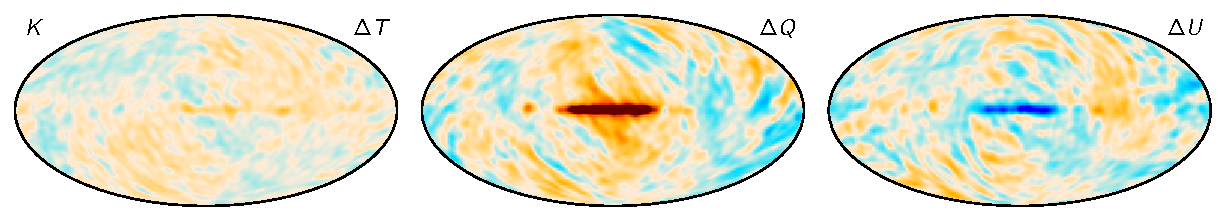
\includegraphics[width=\textwidth]{figures/023-WMAP_K_sampdiff.pdf}\\
	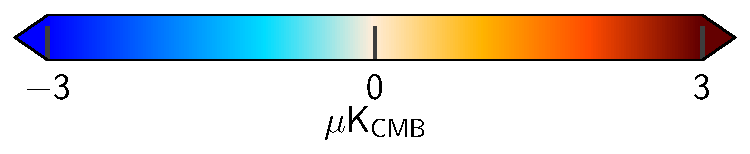
\includegraphics[width=0.30\textwidth]{figures/cbar_3uK.pdf}        
	\caption{Difference between two \K-band Gibbs samples, smoothed to $7^\circ$.}
        \label{fig:Ksampdiff}
\end{figure*}

\begin{figure*}[t]
	\centering
	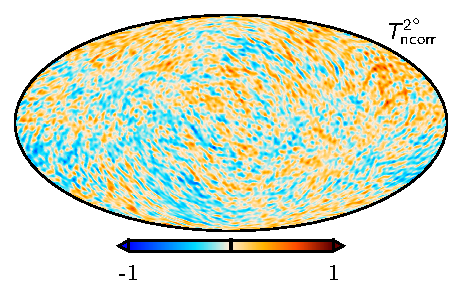
\includegraphics[width=0.32\textwidth]{figures/K_ncorr_I.pdf}
	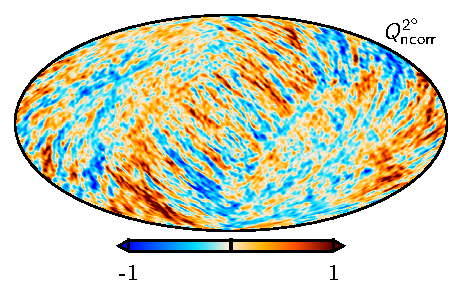
\includegraphics[width=0.32\textwidth]{figures/K_ncorr_Q.pdf}
	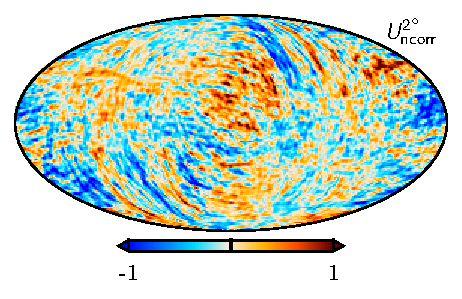
\includegraphics[width=0.32\textwidth]{figures/K_ncorr_U.pdf}\\
	\includegraphics[width=0.32\textwidth]{figures/K_orb_I.pdf}
	\includegraphics[width=0.32\textwidth]{figures/K_orb_Q.pdf}
	\includegraphics[width=0.32\textwidth]{figures/K_orb_U.pdf}\\
	\includegraphics[width=0.32\textwidth]{figures/K_leak_I.pdf}
	\includegraphics[width=0.32\textwidth]{figures/K_leak_Q.pdf}
	\includegraphics[width=0.32\textwidth]{figures/K_leak_U.pdf}\\
	\includegraphics[width=0.32\textwidth]{figures/K_sl_I.pdf}
	\includegraphics[width=0.32\textwidth]{figures/K_sl_Q.pdf}
	\includegraphics[width=0.32\textwidth]{figures/K_sl_U.pdf}\\
	\includegraphics[width=0.32\textwidth]{figures/K_res_I.pdf}
	\includegraphics[width=0.32\textwidth]{figures/K_res_Q.pdf}
	\includegraphics[width=0.32\textwidth]{figures/K_res_U.pdf}\\
	\caption{TOD corrections for \K-band for a single Gibbs sample, projected into maps. Columns show Stokes $T$, $Q$, and $U$ parameters. Rows show, from top to bottom, 1) correlated noise; 2) the orbital dipole; 3); bandpass mismatch leakage; and 4) sidelobe corrections. The bottom row shows the residual obtained when binning the sky and systematics-subtracted TOD into a sky map. Note that the correlated noise and residual have been smoothed by a $2^\circ$ Gaussian beam.}
	\label{fig:tod_corrections}
\end{figure*}

\begin{figure*}
  \center	
   \includegraphics[width=0.95\linewidth]{figures/components_power_spectrum_std_masked_WMAP_new_rms.pdf}
  \caption{Pseudo-spectrum standard deviation for each instrumental
    systematic correction shown in
    Fig.~\ref{fig:tod_corrections} (\emph{thin
      colored lines}). For comparison, thick black lines show spectra
    for the full coadded frequency map; thick red lines show the
    standard deviation of the same (i.e., the full systematic
    uncertainty); gray lines show white noise realizations; and black lines
    show the power spectra of the maps themselves. Columns show results for \K,
    \Ka, \Q1, and \W4, respectively, while rows show results for each of
    the six polarization states ($TT$, $EE$, $BB$, $TE$, $TB$, and
    $EB$). All spectra have been derived outside the CMB confidence
    mask presented by \citet{bp13} using the HEALPix \texttt{anafast}
    utility, correcting only for sky fraction and not for mask mode
    coupling. }
  \label{fig:corrmap_stddev}
\end{figure*}

%\begin{figure*}[t]
%	\centering
%	\includegraphics[width=\textwidth]{figures/tod_res_K_IQU.pdf}\\
%	\includegraphics[width=0.30\textwidth]{figures/cbar_5uK.pdf}        
%	\caption{\K-band TOD residual, smoothed with by $5^\circ$.}
%        \label{fig:Kres}
%\end{figure*}






%\subsection{Angular power spectra}

%Will combine these spectra shortly
As a final inspection of the \cosmoglobe\ map products, we take the angular power spectra of the maps themselves and compare with the \WMAPnine\ results in Fig.~\ref{fig:map_spectra}. To compute the power spectrum, we mask the data using the extended temperature analysis mask which allows a sky fraction of 68.8\,\% and obtain the pseudo-$C_\ell$ power spectra using the \texttt{NaMaster} \citep{namaster}\footnote{\url{https://github.com/LSSTDESC/NaMaster}} \texttt{compute\_full\_master} routine, returning a set of decoupled bandpowers.

As the temperature power spectra are signal-dominated up to $\ell\sim200$ for all DAs, it is more useful to look at the ratio of spectra in the left column of Fig.~\ref{fig:map_spectra}. Here we see that the spectra are consistent with each other at all but the very largest and smallest scales. The largest scale differences are due to mode-coupling effects -- the \WMAPnine\ maps were produced by removing the Solar dipole in the timestream before mapmaking, while the \cosmoglobe\ maps needed a dipole estimate to be removed as a post-processing step. The small scale differences above $\ell\sim200$ can be attributed to the white noise treatment. In particular, the \WMAPnine\ processing gain solution varies every 23\,s compared to the \cosmoglobe\ solution which uses constant gain per scan. Conversely, the \cosmoglobe\ radiometer noise estimate varies per scan, whereas there is no mention of raw instrumental noise variation with time in the \WMAP\ suite of papers.


%\begin{figure*}
%	\centering
%	\includegraphics[width=0.8\textwidth]{figures/TT_spectra.pdf}
%	\caption{TT power spectra}
%	\label{fig:tt_cg}
%\end{figure*}
%\begin{figure*}
%	\centering
%	\includegraphics[width=0.8\textwidth]{figures/TT_spectra_ratio.pdf}
%	\caption{TT ratios}
%	\label{fig:tt_ratio}
%\end{figure*}

The $E$-mode power spectra, displayed in the second column of Fig.~\ref{fig:map_spectra}, are mainly dominated by noise and polarized synchrotron emission. As expected, the large scale foreground-dominated multipoles decrease in amplitude according to the relative amplitude of the synchrotron spectrum. Aside from the $\ell=8$ \W2 multipole, the \cosmoglobe\ power spectra are well-behaved across all bands. The large fluctuations in the \WMAP\ power spectrum, in particular \W2 and \W4, are almost completely gone in the \cosmoglobe\ analysis.

The $B$-mode power spectra, displayed in the third column of Fig.~\ref{fig:map_spectra}, should follow the same pattern as in the $E$-modes, but with foregrounds reduced by a factor of $\simeq2$ \citep{bennett2012}. Indeed, with the notable exception of the \Ka\ and \Q1 $\ell=3$ multipoles and the \W3 $\ell=7$ multipole, this pattern is largely borne out, with nearly white noise across all angular scales. The $C_{\ell=3}^\mathrm{BB}$ mode has been identified as being poorly measured by, e.g., \citet{jarosik2010}, due to its symmetry aligning with $\gtrsim10\,\mathrm{min}$ signals in the TOD induced by the \WMAP\ scan strategy.

In general, we find that the reprocessed \WMAP\ maps produced in the \cosmoglobe\ framework have map and power spectrum properties that contain traces of the \WMAP\ observation strategy than the \WMAPnine\ products. To fully assess the quality of these frequency maps compared to the official \WMAPnine\ products, we compare the maps explicitly in Sect.~\ref{sec:wmap_comparison}.



%\begin{figure*}
%	\centering
%	\includegraphics[width=0.8\textwidth]{figures/EE_spectra.pdf}
%	\caption{EE power spectra}
%	\label{fig:ee_cg}
%\end{figure*}
%\begin{figure*}
%	\centering
%	\includegraphics[width=0.8\textwidth]{figures/BB_spectra.pdf}
%	\caption{BB power spectra}
%	\label{fig:bb_cg}
%\end{figure*}

\begin{figure*}
	\centering
	\includegraphics{figures/TT_ratio.pdf}
	\includegraphics{figures/EE_BB_spec.pdf}
	\caption{Comparison of the $C_\ell^\mathrm{TT}$, $C_\ell^\mathrm{EE}$, and $C_\ell^\mathrm{BB}$ from \WMAPnine\ and \cosmoglobe. Each row corresponds to a different DA, with frequency increasing from top to bottom. \textit{(left):} ratio of $C_\ell^\mathrm{TT}$ from \cosmoglobe\ compared to \WMAPnine. \textit{(middle/right):} $C_\ell^\mathrm{EE/BB}$ power spectra with \WMAPnine\ in blue and \cosmoglobe\ in orange.}
	\label{fig:map_spectra}
\end{figure*}


\subsection{Comparison with 9-year \WMAP\ maps}
\label{sec:wmap_comparison}

\begin{figure*}
	\centering
	\includegraphics[width=0.32\textwidth]{figures/megadiff_K_I.pdf}
        \includegraphics[width=0.32\textwidth]{figures/megadiff_K_Q.pdf}
        \includegraphics[width=0.32\textwidth]{figures/megadiff_K_U.pdf}\\\vspace*{-4mm}
	\includegraphics[width=0.32\textwidth]{figures/megadiff_Ka_I.pdf}
        \includegraphics[width=0.32\textwidth]{figures/megadiff_Ka_Q.pdf}
        \includegraphics[width=0.32\textwidth]{figures/megadiff_Ka_U.pdf}\\\vspace*{-4mm}
	\includegraphics[width=0.32\textwidth]{figures/megadiff_Q_I.pdf}
        \includegraphics[width=0.32\textwidth]{figures/megadiff_Q_Q.pdf}
        \includegraphics[width=0.32\textwidth]{figures/megadiff_Q_U.pdf}\\\vspace*{-4mm}
	\includegraphics[width=0.32\textwidth]{figures/megadiff_V_I.pdf}
        \includegraphics[width=0.32\textwidth]{figures/megadiff_V_Q.pdf}
        \includegraphics[width=0.32\textwidth]{figures/megadiff_V_U.pdf}\\\vspace*{-4mm}
	\includegraphics[width=0.32\textwidth]{figures/megadiff_W_I.pdf}
        \includegraphics[width=0.32\textwidth]{figures/megadiff_W_Q.pdf}
        \includegraphics[width=0.32\textwidth]{figures/megadiff_W_U.pdf}\\\vspace*{-4mm}
	\includegraphics[width=0.32\textwidth]{figures/cbar_5uK_cmb.pdf}
	\caption{Difference maps between the \cosmoglobe\ and 9-year \WMAP\ frequency maps. Columns show Stokes $T$, $Q$, and $U$ parameter maps, while rows show \K-, \Ka-, \Q-, \V-, and \W-band maps. The maps are all smoothed with a $2^\circ$ FWHM Gaussian beam.}
        \label{fig:megadiff_wmap}
\end{figure*}

We present difference maps between the official 9-year \WMAP\ maps and the maps produced in this work in Fig.~\ref{fig:megadiff_wmap}. This figure shows a total of fifteen difference maps, one for each of the main \WMAP\ bands (\K, \Ka, \Q, \V, and \W), in the three Stokes parameters. 

The differences are overall quite small, as the data processing between \cosmoglobe\ and \WMAPnine\ are quite similar, with subtle differences as described in Sec.~\ref{sec:data}. In total intensity, we see good agreement with the full \WMAPnine\ results, with deviations at the few $\mu\mathrm{K}$ level. The largest difference between the two analyses is shown in the \K-band difference map, which demonstrates the difference between the band calibration as described in Sects.~\ref{sec:gain} and \ref{sec:ame_Kband}.
This can be attributed to the absolute calibration differences between the two pipelines. In particular, \citet{bennett2012} estimates a calibration uncertainty of 0.2\,\% across all bands, corresponding to a $\sim7\,\mathrm{\mu K}$ variation in the Solar dipole amplitude.
On the other hand, the  \cosmoglobe\ absolute calibration prior width of 0.002 can induce a $6\,\mathrm{\mu K}$ Solar dipole residual. Therefore, a dipole difference such as this is not unexpected.
In bands \Ka--\W, the absolute calibration is driven wholly by the sampling algorithms descrbed in Sect.~\ref{ssec:oldsamplers}, and as such is much more susceptible to poor modeling of the data. The fact then that the dipole amplitude in the difference maps is so small is strong evidence that the parametric modeling of the absolute calibration performance is comparable to the \WMAPnine\ approach of modelling the gain using on-board thermistors.

In the \V\ and \W-band temperature maps, there is an additional quadrupole signal closely aligned with the Solar dipole. As noted in \citet{larson2014}, the \WMAPnine\ maps retain the kinematic quadrupole, whereas \commanderthree\ removes this component. While kinematic quadrupole has the expected shape, the frequency dependence is not consistent with the expected functional form $x\coth x$ where $x=h\nu/(2kT_\mathrm{CMB})$ \citep{Notari:2015}. It is therefore likely that the quadrupole difference comes from some second-order effects in the time variation of the gain. There is indeed an oscillatory structure in the relative difference between the gain solutions, which can be most seen in Fig.~\ref{fig:dgain}.



In polarization, we note large scale differences in both Stokes $Q$ and $U$. These large scale differences do not match known Galactic component morphologies. All of these differences are well-described by linear combinations of the  poorly measured modes, though the map-space morphologies are not identical. These large mode differences are due to three main effects: 1) poor polarization angle coverage for a few large-scale modes; 2) errors in transmission imbalance coupled with the Solar dipole; and 3) interplay between the transmission imbalance, the far sidelobe, and the Solar dipole, as briefly described in Sect.~\ref{sec:official_pipeline}. The scale of these effect is most pronounced in the \W-band polarization results, where we see the largest differences between the two processing pipelines.

The removal of the poorly measured modes demonstrates the benefit of jointly processing these two experiments simultaneously in the same framework. The differences shown in Fig.~\ref{fig:megadiff_wmap}, particularly in polarization, are due to effects in the \WMAPnine\ maps that cannot be constrained by the \WMAP\ observation strategy. 
Instead, in the joint analysis, the full sky model allows for a framework in which large scale modes,
clearly not Galactic in origin, to be attributed to the combination of imbalance parameter and Solar dipole uncertainty. 
%work, these modes would either be clearly present in Galactic component maps, or in the component separation residuals (Sect.~\ref{sec:astrophysics}, Fig.~\ref{fig:compsep_residual}) and they are present in neither. 


%\textit{Comment on the differences} -- the kinematic quadrupole is not removed in the \WMAPnine\ maps \citep{larson2014}, and the amplitude goes as $\nu/(2T_0)\coth(\nu/(2T_0))$ \citep{Notari:2015}.

\begin{table}
\newdimen\tblskip \tblskip=5pt
\caption{Difference map $\chi^2$ statistics.  }
\label{tab:chisq}
\vskip -4mm
\footnotesize
\setbox\tablebox=\vbox{
 \newdimen\digitwidth
 \setbox0=\hbox{\rm 0}
 \digitwidth=\wd0
 \catcode`*=\active
 \def*{\kern\digitwidth}
%
  \newdimen\dpwidth
  \setbox0=\hbox{.}
  \dpwidth=\wd0
  \catcode`!=\active
  \def!{\kern\dpwidth}
%
  \halign{\hbox to 2.5cm{#\leaderfil}\tabskip 2em&
    \hfil$#$\hfil \tabskip 2em&
    \hfil$#$\hfil \tabskip 2em&    
    \hfil$#$\hfil \tabskip 0em\cr
\noalign{\doubleline}
\omit\hfil\sc Difference \hfil& \chi^2_{\mathrm{uncorr}} & \chi^2_{\mathrm{corr}} & \Delta \chi^2\cr
\noalign{\vskip 3pt\hrule\vskip 5pt}
$0.32\times$K1 $-$ Ka1  & 4291  & 4287  & **4 \cr
Q1 $-$ Q2         & 4500  & 4380  & 120 \cr
V1 $-$ V2         & 4490  & 4429  & *61 \cr
W1 $-$ W2         & 4328  & 4270  & *68 \cr
W3 $-$ W4         & 4257  & 4145  & 112 \cr
\noalign{\vskip 5pt\hrule\vskip 5pt}}}
\endPlancktablewide
\end{table}


\begin{table}
\newdimen\tblskip \tblskip=5pt
\caption{Transmission imbalance template amplitudes for each \WMAP\ radiometer as estimated by fitting the official templates to low-resolution difference maps between \cosmoglobe\ and \WMAP. The templates are provided in mK, and the template amplitudes are therefore dimensionless. The fourth column lists the relative decrease in standard deviation, $\sqrt{\sigma_{\mathrm{raw}}^2 - \sigma_{\mathrm{corr}}^2}/\sigma_{\mathrm{raw}}$,  after subtracting the best-fit templates in percent. }
\label{tab:transmission}
\vskip -4mm
\footnotesize
\setbox\tablebox=\vbox{
 \newdimen\digitwidth
 \setbox0=\hbox{\rm 0}
 \digitwidth=\wd0
 \catcode`*=\active
 \def*{\kern\digitwidth}
%
  \newdimen\dpwidth
  \setbox0=\hbox{.}
  \dpwidth=\wd0
  \catcode`!=\active
  \def!{\kern\dpwidth}
%
  \halign{\hbox to 1.8cm{#\leaderfil}\tabskip 2em&
    \hfil$#$\hfil \tabskip 2em&
    \hfil$#$\hfil \tabskip 2em&    
    \hfil$#$\hfil \tabskip 0em\cr
\noalign{\doubleline}
\omit\hfil\sc DA \hfil& a_1 & a_2 & \Delta \sigma [\%]\cr
\noalign{\vskip 3pt\hrule\vskip 5pt}
K1 &   -27.5*  &  -50.6* & 30 \cr
Ka1 &   -1.4  &   -1.9 & 25 \cr
Q1 &   -30.0* &  -71.6* & 11 \cr
Q2 &   -7.1  &  -1.5 & 20 \cr
V1 &   -32.8*  &  -53.4* & *6 \cr
V2 &   *8.8  &  -4.1 & 16 \cr
W1 &   -2.8  &  *4.6 & *8 \cr
W2 &   -6.9  & -3.5 & 11 \cr
W3 &   29.1  & 53.4 & 12 \cr
W4 &   15.5  & -6.8 & 52 \cr
\noalign{\vskip 5pt\hrule\vskip 5pt}}}
\endPlancktablewide
\end{table}




\subsection{Consistency within \WMAP\ channels}
\label{sec:internal_consistency}

An important test for how well the instrumental systematics are being modeled is by checking the agreement within each of the \WMAP\ channels. As described in Sect.~\ref{sec:official_pipeline}, the \Q-band and \V-band channels each had two DAs, while the \W-band had four DAs. Checking for discrepancies between each of the individual DA maps within the same frequency channel can highlight mismodeled systematics. While the \K-band and \Ka-band have different central frequencies, they are close enough that we can compare them by scaling \K-band assuming a polarized synchrotron power law of $\beta_\mathrm s=-3.1$.

The interchannel maps for Stokes $Q$ and $U$ are shown in Fig.~\ref{fig:internal_diff}. 
For the \K-\Ka\ difference, there are coherent signals in both the \WMAPnine\ and \cosmoglobe\ difference maps. An unsurprising difference is along the Galactic plane, due to the sky not being well-described by a simple global power law in this region. However, the large-scale Stokes $Q$ map has a large scale residual that is not matched in $U$. This coherent structure is present in both the \WMAPnine\ and \cosmoglobe\ maps, although in \WMAPnine\ the structure is interrupted by the poorly measured modes. In comparison, the \cosmoglobe\ $U$ map has much less large-scale structure than the \WMAPnine\ difference map.

The internal DA differences provide a cleaner comparison, with no astrophysical assumptions required. The \Q-band and \V-band half-difference maps from \cosmoglobe\ have virtually no trace of the poorly measured modes, and the difference patterns are well-traced by the rms maps, with smaller differences at the ecliptic poles and larger differences along the ecliptic plane. The largest visual improvement is in the \W-band half-difference, where the \cosmoglobe\ case is almost entirely consistent with white noise, as opposed to the \WMAPnine\ difference that is dominated by the poorly measured modes.  Based on these visual comparisons, the \cosmoglobe\ maps themselves contain essentially none of the poorly-measured modes and are more self-consistent than the \WMAPnine\ frequency maps.


\begin{figure*}
	\centering
	\includegraphics[width=0.24\textwidth]{figures/KKa_deltaQ.pdf}
	\includegraphics[width=0.24\textwidth]{figures/KKa_W_deltaQ.pdf}
	\includegraphics[width=0.24\textwidth]{figures/KKa_deltaU.pdf}
	\includegraphics[width=0.24\textwidth]{figures/KKa_W_deltaU.pdf}\\
	\includegraphics[width=0.24\textwidth]{figures/Q_deltaQ.pdf}
	\includegraphics[width=0.24\textwidth]{figures/Q_W_deltaQ.pdf}
	\includegraphics[width=0.24\textwidth]{figures/Q_deltaU.pdf}
	\includegraphics[width=0.24\textwidth]{figures/Q_W_deltaU.pdf}\\
	\includegraphics[width=0.24\textwidth]{figures/V_deltaQ.pdf}
	\includegraphics[width=0.24\textwidth]{figures/V_W_deltaQ.pdf}
	\includegraphics[width=0.24\textwidth]{figures/V_deltaU.pdf}
	\includegraphics[width=0.24\textwidth]{figures/V_W_deltaU.pdf}\\
	\includegraphics[width=0.24\textwidth]{figures/W_deltaQ.pdf}
	\includegraphics[width=0.24\textwidth]{figures/W_W_deltaQ.pdf}
	\includegraphics[width=0.24\textwidth]{figures/W_deltaU.pdf}
	\includegraphics[width=0.24\textwidth]{figures/W_W_deltaU.pdf}
        \includegraphics[width=0.25\textwidth]{figures/cbar_10uK.pdf}
	\caption{Internal \WMAP\ difference maps, smoothed by $10^\circ$. The two left columns are Stokes $Q$, and the two right columns are Stokes $U$, with the \cosmoglobe\ and \WMAPnine\ maps alternating between columns. The top to bottom rows are difference maps in increasing frequency.}
	\label{fig:internal_diff}
\end{figure*}


As noted by \citet{jarosik2010}, the low-$\ell$ \W-band polarization data were excluded from cosmological analysis due to excess variance in the $\ell\leq7$ multipoles. To test the \cosmoglobe\ maps' performance at these scales, we take the power spectrum of the full-sky difference maps using the standard \texttt{anafast} routine in Fig.~\ref{fig:cl_halfdiff}. With very few exceptions, the \WMAPnine\ power spectra have much more power at $\ell\leq7$ than the \cosmoglobe\ maps in both the $E$-modes and $B$-modes. Of particular note is the $\ell=3$ $B$-mode, which has consistently been identified as poorly measured in the \WMAP\ scan strategy, and has been reduced in every difference spectrum. Based on these power spectra, we can identify no reason to exclude the reprocessed \W-band polarization data in future cosmological analyses.


\begin{figure}
	\centering
	\includegraphics[width=\linewidth]{figures/cls_cg_WMAP_lowl.pdf}
	\caption{Full sky half-difference spectra. The red lines are the power spectra of the \WMAPnine\ difference maps, while the black lines are the same for the reprocessed \cosmoglobe\ maps.}
        \label{fig:cl_halfdiff}
\end{figure}



\subsection{Consistency between \WMAP\ and LFI}
\label{sec:lfi_consistency}


As \WMAP\ and LFI observe an overlapping frequency range, it is vital to assess
how well these two experiments agree with each other, as the sky they observe
is the same. Inspecting comparisons of the two experiments' sky maps can help
elucidate differences between them induced by scan strategy and instrument
design. Figure~\ref{fig:wmap_lfi_compare} shows comparisons between the \WMAP\
$K$- and $Ka$-bands and the LFI 30 GHz channel, between the \WMAP\ $Q$-band and
LFI 44 GHz, and finally between \WMAP\ $V$-band and LFI 70 GHz. For
demonstration, the sky maps produced in this work are compared against the
offical \WMAPnine\ and \BP\ maps. Additionally, we compare the mean \W-band
maps with the DR4 100\,GHz channel. In this comparison, the HFI map has had no
input from \commanderthree\ so this difference map is an independent comparison
between two datasets and processing methods.

Starting with the \cosmoglobe\ maps, we see in the first and third columns of
Fig.~\ref{fig:wmap_lfi_compare} that the magnitude of the differences are small
in both Stokes $Q$ and $U$. Overall, across all five frequency map comparisons
we see small levels of variation, with structure contained to the Galactic
plane. Notably, however, there is a larger sky signal within the
$\mathit{Ka}-30$ Stokes $Q$ comparison.  This deviation is consistent with that
from the $\mathit{Ka}-\mathit{K}$ comparison in Fig.~\ref{fig:internal_diff}.
The fact that this difference persists between these two difference maps
indicates that this large-scale signal is confined to \Ka, and is due either to
data processing artifacts unique to this DA or to unmodeled sky polarization in
the \Ka\ bandpass. This large-scale difference also exists in the $\mathit
Q-44$ Stokes $Q$, but did not appear in the internal \Q\ half-difference map.
This strengthens the hypothesis that the signal is on the sky, but could still
be a result of \WMAP\ data processing, as the signal consistently appears in
the \WMAP\ data.  Overall, across all frequency map comparisons, deviations at
high Galactic latitudes are low, demonstrating a robust ability to remove
poorly measured modes from both experiments thanks to the joint processing. The
clearest improvement in reprocessing is shown in the final row of
Fig.~\ref{fig:wmap_lfi_compare}. The structure of the \cosmoglobe\ difference
maps in both Stokes $Q$ and $U$ shows ery low levels of variation, in both the
Galactic plane and at high latitudes. 


Columns two and four of Fig.~\ref{fig:wmap_lfi_compare} show the differences
between the official \WMAPnine\ and \BP\ LFI frequency maps. Similar to the
\cosmoglobe\ sky map comparisons, we see differences in the Galactic center,
and to a lesser degree along the Galactic plane due to the slight differences
in the frequency coverage. When comparing the official \WMAP\ maps,
particularly for \K-band, we see structures sweeping across large angular
scales across the sky, likely due to the poorly measured modes in \K-band. 
These structures were noted within the
\BP\ project, particularly in the polarized component separation and
large-scale polarized AME studies \citep{bp14,bp15}. 


Of particular note is the $100-\mathit W$ difference map. The \cosmoglobe\
difference maps here have a similar level of white noise and Galactic
contamination as the $\mathit V-70$ maps,  whereas the \WMAPnine\ differences
are driven by the transmission imbalance modes, each with an opposite sign and
magnitude. The difference between 100\,GHz and \W\ demonstrates that the good
agreement between the \WMAP\ and \Planck\ LFI is not simply due to fitting
low-level parameters in a joint analysis framework -- by obtaining \W-band maps
that are consistent with an independent 100\,GHz polarization map, we have
shown that the \WMAP\ is not simply the result of adding more free parameters
to the fit, but a genuine improvement in data processing.



\begin{figure*}
	\centering
	\includegraphics[width=0.24\textwidth]{figures/K30_deltaQ.pdf}
	\includegraphics[width=0.24\textwidth]{figures/K30_W_deltaQ.pdf}
	\includegraphics[width=0.24\textwidth]{figures/K30_deltaU.pdf}
	\includegraphics[width=0.24\textwidth]{figures/K30_W_deltaU.pdf}\\
	\includegraphics[width=0.24\textwidth]{figures/30Ka_deltaQ.pdf}
	\includegraphics[width=0.24\textwidth]{figures/30Ka_W_deltaQ.pdf}
	\includegraphics[width=0.24\textwidth]{figures/30Ka_deltaU.pdf}
	\includegraphics[width=0.24\textwidth]{figures/30Ka_W_deltaU.pdf}\\
	\includegraphics[width=0.24\textwidth]{figures/44Q_deltaQ.pdf}
	\includegraphics[width=0.24\textwidth]{figures/44Q_W_deltaQ.pdf}
	\includegraphics[width=0.24\textwidth]{figures/44Q_deltaU.pdf}
	\includegraphics[width=0.24\textwidth]{figures/44Q_W_deltaU.pdf}\\
	\includegraphics[width=0.24\textwidth]{figures/70V_deltaQ.pdf}
	\includegraphics[width=0.24\textwidth]{figures/70V_W_deltaQ.pdf}
	\includegraphics[width=0.24\textwidth]{figures/70V_deltaU.pdf}
	\includegraphics[width=0.24\textwidth]{figures/70V_W_deltaU.pdf}\\
	\includegraphics[width=0.24\textwidth]{figures/100W_deltaQ.pdf}
	\includegraphics[width=0.24\textwidth]{figures/100W_W_deltaQ.pdf}
	\includegraphics[width=0.24\textwidth]{figures/100W_deltaU.pdf}
	\includegraphics[width=0.24\textwidth]{figures/100W_W_deltaU.pdf}
	
        \includegraphics[width=0.25\textwidth]{figures/cbar_10uK.pdf}
	\caption{Difference maps between similar \WMAP\ and \Planck\ frequency maps. The comparison plots go, by column: Stokes $Q$ for the \cosmoglobe\ sky maps, Stokes $Q$ for official \WMAP\ and \BP\ data products, Stokes $U$ for the \cosmoglobe sky maps, and Stokes $U$ for the official data products. (Top row) \WMAP\ LFI 30 GHz minus \K-band, scaled by the synchrotron power-law. (Top middle row) \WMAP\ \Ka-band minus LFI 30 GHz, also scaled by the synchrotron power-law. (Middle row) \WMAP\ \Q-band compared to the LFI 44 GHz sky maps, scaled by the synchrotron power-law. (Bottom middle row) \WMAP\ \V-band minus LFI 70 GHz, with unit scalings for each band. (Bottom row) The \Planck\ DR4 100 GHz map minus the \WMAP\ \W-band\, also with unit scalings for each band.}
	\label{fig:wmap_lfi_compare}
\end{figure*}


\section{Preliminary astrophysical results}
\label{sec:astrophysics}

In this section, we present initial results for the astrophysical component separation temperature power spectra. The frequency coverage in this analysis is essentially the same as \bp, with the notable addition of the high signal-to-noise \K-band and the reprocessed \W-band. As such, the results presented here are similar in quality to the results presented in \citet{bp01}.

\subsection{CMB results}
\label{sec:cmb}

Cosmological parameter estimation is left for future work, in large part because the two chains of length 250 are too short to reliably estimate cosmological parameters in this framework. For comparison, \citet{bp12} demonstrated that at least 2000 Gibbs samples were required before the reionizaiton optical depth $\tau$ value had converged. Similarly, for \bp\ in the temperature case, the Gelman-Rubin statistic is just above $R=1.01$ for $\ell\lesssim600$ then continues to increase, indicating marginally acceptable convergence across all multipoles. Therefore, the results for the CMB presented here serve mainly as consistency checks. Given these caveats, we present preliminary CMB analysis in Sects.~\ref{sec:dipole}--\ref{sec:cls}.





\begin{figure*}
	\centering
	\includegraphics[width=0.8\textwidth]{figures/cmb_I_dipole.pdf}
	\caption{Posterior mean CMB \cosmoglobe\ temperature map, smoothed to an angular resolution of $14'$ FWHM.}
\end{figure*}

\begin{figure*}
	\includegraphics[width=0.33\textwidth]{figures/cmb_I_nodipole.pdf}
	\includegraphics[width=0.33\textwidth]{figures/cmb_Q.pdf}
	\includegraphics[width=0.33\textwidth]{figures/cmb_U.pdf}\\
	\includegraphics[width=0.33\textwidth]{figures/cmb_I_sigma.pdf}
	\includegraphics[width=0.33\textwidth]{figures/cmb_Q_sigma.pdf}
	\includegraphics[width=0.33\textwidth]{figures/cmb_U_sigma.pdf}\\
	\caption{Posterior mean CMB \cosmoglobe\ maps and their standard deviation.}
\end{figure*}

\subsubsection{Solar dipole}
\label{sec:dipole}


\begin{table*}
\newdimen\tblskip \tblskip=5pt
\caption{Comparison of Solar dipole measurements from \COBE, \WMAP, and \Planck. }
\label{tab:dipole}
\vskip -4mm
\footnotesize
\setbox\tablebox=\vbox{
 \newdimen\digitwidth
 \setbox0=\hbox{\rm 0}
 \digitwidth=\wd0
 \catcode`*=\active
 \def*{\kern\digitwidth}
%
  \newdimen\dpwidth
  \setbox0=\hbox{.}
  \dpwidth=\wd0
  \catcode`!=\active
  \def!{\kern\dpwidth}
%
  \halign{\hbox to 2.5cm{#\leaderfil}\tabskip 2em&
    \hfil$#$\hfil \tabskip 2em&
    \hfil$#$\hfil \tabskip 2em&
    \hfil$#$\hfil \tabskip 2em&
    #\hfil \tabskip 0em\cr
\noalign{\doubleline}
\omit&&\multispan2\hfil\sc Galactic coordinates\hfil\cr
\noalign{\vskip -3pt}
\omit&\omit&\multispan2\hrulefill\cr
\noalign{\vskip 3pt} 
\omit&\omit\hfil\sc Amplitude\hfil&l&b\cr
\omit\hfil\sc Experiment\hfil&[\muK_{\rm
CMB}]&\omit\hfil[deg]\hfil&\omit\hfil[deg]\hfil&\hfil\sc Reference\hfil\cr
\noalign{\vskip 3pt\hrule\vskip 5pt}
\COBE \rlap{$^{\rm a,b}$}&                  3358!**\pm23!**&     264.31*\pm0.16*&
     48.05*\pm0.09*&\citet{lineweaver1996}\cr
\WMAP\ \rlap{$^{\rm c}$}&                  3355!**\pm*8!**&     263.99*\pm0.14*&
     48.26*\pm0.03*&\citet{hinshaw2009}\cr
\noalign{\vskip 3pt}
LFI 2015 \rlap{$^{\rm b}$}&              3365.5*\pm*3.0*&     264.01*\pm0.05*&
     48.26*\pm0.02*&\citet{planck2014-a03}\cr
HFI 2015 \rlap{$^{\rm d}$}&              3364.29\pm*1.1*&     263.914\pm0.013&
     48.265\pm0.002&\citet{planck2014-a09}\cr
\noalign{\vskip 3pt}
LFI 2018 \rlap{$^{\rm b}$}&              3364.4*\pm*3.1*&     263.998\pm0.051&
     48.265\pm0.015&\citet{planck2016-l02}\cr
HFI 2018 \rlap{$^{\rm d}$}&              3362.08\pm*0.99&     264.021\pm0.011&
     48.253\pm0.005&\citet{planck2016-l03}\cr
\noalign{\vskip 3pt}
Bware & 3361.90\pm*0.40 & 263.959\pm0.019 & 48.260\pm0.008  & \citet{delouis:2021}  \cr
\Planck\ PR4\ \rlap{$^{\rm a,c}$}& 3366.6*\pm*2.6*& 263.986\pm0.035&
48.247\pm0.023&\citet{planck2020-LVII}\cr
\noalign{\vskip 3pt}
\BP\ \rlap{$^{\rm e}$} & 3362.7*\pm*1.4*& 264.11*\pm0.07*&
 48.279\pm0.026&\citet{bp11}\cr
\noalign{\vskip 3pt}
\bf\cosmoglobe\ \rlap{$^{\rm e}$} & \bf3366.2*\pm*1.4*& \bf264.08*\pm0.07*&
 \bf48.273\pm0.024&This work\cr
\noalign{\vskip 5pt\hrule\vskip 5pt}}}
\endPlancktablewide
\tablenote {{\rm a}} Statistical and systematic uncertainty estimates are added in quadrature.\par
\tablenote {{\rm b}} Computed with a naive dipole estimator that does not account for higher-order CMB fluctuations.\par
\tablenote {{\rm c}} Computed with a Wiener-filter estimator that estimates, and marginalizes over, higher-order CMB fluctuations jointly with the dipole.\par
\tablenote {{\rm d}} Higher-order fluctuations as estimated by subtracting a dipole-adjusted CMB-fluctuation map from frequency maps prior to dipole evaluation. \par
\tablenote {{\rm e}} Estimated with a sky fraction of 68\,\%. Error bars include only statistical uncertainties, as defined by the global \cosmoglobe\ posterior framework, and they thus account for instrumental noise, gain fluctuations, parametric foreground variations etc. 
\par
\end{table*}

As argued by \citet{thommesen:2019}, estimating the Solar dipole is one of the more difficult parameters to accurately constrain. This is in part due to the effect of mode-coupling when masking the Galactic plane, but also due to the Solar dipole in the calibration step. In essence, the Solar dipole's amplitude couples strongly to the calibration parameters. Misestimation of the calibration can propagate to an incorrect CMB dipole, and vice-versa.

The results of our Solar dipole estimate are displayed in Table~\ref{tab:dipole} and Fig.~\ref{fig:dip_amp}. We find that the dipole direction is consistent with the \citet{bp11} result, but is $11\,\mathrm{\mu K}$ higher than the result from \citet{hinshaw2009}. Assuming a $3400\,\mathrm{\mu K}$ Solar dipole amplitude, an absolute calibration error of $0.3\,\%$ is sufficient to to induce an $11\,\mathrm{\mu K}$ error. In fact, the 0.2\,\% absolute calibration error reported by \citet{bennett2012} can induce a $6.7\,\mathrm{\mu K}$ Solar dipole amplitude error, dominating the error budget for the final reported Solar dipole.

\begin{figure}
	\includegraphics[width=\columnwidth]{figures/dip_amplitude.pdf}
	\caption{CMB dipole amplitude as a function of sky fraction. The gray band indicates the 68\,\% posterior confidence region.}
	\label{fig:dip_amp}
\end{figure}

It is also noteworthy that the \bp\ Solar dipole differs from the \cosmoglobe\ Solar dipole with a higher significance even than the \WMAPnine\ result, despite using a nearly identical framework and almost identical datasets. First, we note that the \Planck\ PR4 analysis \citep{npipe} showed a similarly apparently paradoxical discrepancy. On its face, the LFI 2018 and HFI 2018 Solar dipole values would average according to their uncertainties to $\sim3362.3\,\mathrm{\mu K}$. In this analysis, \citet{npipe} identify relative calibration uncertainty between 100 and 143\,GHz as the dominant source of uncertainty.

In the \cosmoglobe\ analysis, we find that \K-band has the highest signal-to-noise among all low freuqency components, while being absolutely calibrated using a prior distribution. Therefore, it is likely that the chosen prior mean directly impacts the final Solar dipole amplitude, as it sets the amplitude of all low frequency components. 





\subsubsection{Angular temperature power spectrum}
\label{sec:cls}

\begin{figure}
	\includegraphics[width=\columnwidth]{figures/cl_TT_CG_v1.pdf}
	\caption{\textit{(Top:)} CMB temperature power spectrum, $D_\ell^\mathrm{TT}$, as derived by \cosmoglobe\ (black), \bp\ (green), \planck\ (red), and \WMAPnine\ (blue). The best-fit \planck\ 2018 \LCDM\ spectrum is showed in dashed gray. \textit{(Middle:)} Residual power spectrum relative to \LCDM, measured relative to the quoted error bars, $(D_\ell-D_\ell^\mathrm{\Lambda CDM})/\sigma_\ell$. For pipelines that report asymmetric error bars, $\sigma_\ell$ is taken to be the average of the upper and lower error bar. \textit{(Bottom:)} Fractional difference with respect to the \planck\ \LCDM\ spectrum. In this panel, each curve has been boxcar averaged with a window of $\Delta\ell=100$ to suppress random fluctuations.}
	\label{fig:cl_tt}
\end{figure}


Figure~\ref{fig:cl_tt} shows the angular temperature power spectrum derived from the CMB samples from the main Gibbs chain, obtained using a Blackwell-Rao estimator \citep{chu2005,bp11}. We compare with the official \WMAP\ \citep{hinshaw2012} and \planck\ \citep{planck2016-l05} power spectra, as well as the \bp\ \citep{bp11} spectrum. For reference, the best-fit \planck\ 2018 \LCDM\ spectrum is plotted along side them. The middle panel shows the deviation from the \planck\ \LCDM\ solution, in units of $\sigma_\ell$ from each individual pipeline, while the bottom panel shows the fractional difference with respect to the \planck\ \LCDM\ spectrum.

At $\ell\lesssim500$, each of these datasets are signal-dominated, and each of the spectra agree at nearly every multipole. Notable exceptions include specifically the quadrupole, which we will discuss in Sect.~\ref{sec:anomalies}, and $50\lesssim\ell\lesssim100$. In the latter, the \cosmoglobe\ multipoles are consistently $\geq5\,\%$ higher than the \LCDM\ solution.

At $\ell\gtrsim500$, the \WMAPnine\ solution becomes noise dominated, and there is much larger variation between the multipoles. While \planck\ and \bp\ mostly agree with the \cosmoglobe\ solution, the convergence properties of the power spectrum are much worse, and would require an order of magnitude more samples to converge \citep{bp11}. We therefore caution against overinterpreting the specific values from the \cosmoglobe\ power spectrum in this regime.


\subsubsection{Low-$\ell$ anomalies}
\label{sec:anomalies}

Even though the CMB is well described by \LCDM, there are several anomalies, especially at low multipoles, that seem to be in tension with \LCDM. As a rule, the existence of these anomalies is not debated, but rather their significance within \LCDM. Indeed, as argued by \citet{bennett2010}, the existence of these anomalies may simply be described using a posteriori predictions rather than confirming pre-existing predictions. The relevant question is not ``How unlikely is \LCDM\ given this effect's existence?'', but rather, ``How unlikely is this effect's existence given \LCDM?''. Additionally, it is difficult in the standard methodology to determine how much of a given effect is due to unmodeled systematic errors. In this section, we use the full propagation of uncertainty to re-evaluate the significance of outstanding low-$\ell$ anomalies,

It has been noted since \COBE-DMR that the quadrupole amplitude of our CMB is lower than expected from \LCDM\ \citep{bennett:1992}. This has later been confirmed in \wmap\ \citep{hinshaw2003a} and \planck\ \citep{planck2013-XV}, but with large discrepancies in mean value and error bars. Here we compare our estimate of the true realization of the quadrupole, $\sigma_2$, with the mean value predicted by \LCDM, $C_2^\mathrm{\Lambda CDM}$. 
From the marginal distribution $P(\sigma_2\mid\data)$, we find that $\sigma_2=120\pm65\,\mathrm{\mu K^2}$, on its face a $\gtrsim14\sigma$ deviation from the \LCDM\ prediction of $C_2^\mathrm{\Lambda CDM}=1064.7\,\mathrm{\mu K^2}$. 
A more meaningful comparison is against the realizations of $\sigma_2$ observed given \LCDM\ compared to the posterior probability distribution $P(\sigma_2\mid\data)$. To evaluate this, we draw $10^5$ simulations of $\sigma_2$ given $C_2^\mathrm{\Lambda CDM}=1064.7\,\mathrm{\mu K^2}$. In Fig.~\ref{fig:quad_realizations}, we show this comparison with the \BP\ and \cosmoglobe\ posterior distributions.
Following \citet{bp11}, we compute the Blackwell-Rao likelihood for the true $C_2$ given the ensemble of observed $\sigma_2$ in Fig.~\ref{fig:blackwell_rao}. From this analysis, we find the probability-to-exceed (PTE) $C_2^\mathrm{\Lambda CDM}$ to be 10\,\% for the \cosmoglobe\ results. In comparison, the \bp\ result had a PTE of 21\,\%. 


\begin{figure}
	\includegraphics[width=\columnwidth]{figures/WMAP_P_sig_d_c.pdf}
	\caption{Histogram of 100 000 realizations of $C_2$ given $C_2^{\Lambda \mathrm{CDM}} = 1064.7$ compared with the measured power spectrum $\sigma_2$ of our universe for \Cosmoglobe\ (black) and \BP\ (blue).}
	\label{fig:quad_realizations}
\end{figure}

\begin{figure}
	\includegraphics[width=\columnwidth]{figures/WMAP_blackwell-rao.pdf}
	\caption{Marginal probability distribution of the ensemble-averaged $C_2$ given the data, $P(C_2|d)$, as measured by \Cosmoglobe\ (black) and \BP\ (blue).}
	\label{fig:blackwell_rao}
\end{figure}

\begin{figure}
	\includegraphics[width=\columnwidth]{figures/WMAP_n_2_n_3.pdf}
	\caption{The quadrupole-octopole alignment of \Cosmoglobe\ compared with \BP.}
\end{figure}

\begin{figure}
	\includegraphics[width=\columnwidth]{figures/WMAP_t_3.pdf}
	\caption{The octopole planarity statistics $t_3$ compared with the \BP\ analysis (blue).}
\end{figure}

\begin{figure}
	\includegraphics[width=\columnwidth]{figures/WMAP_best_q_fit.pdf}
	\caption{Best-fit amplitude, $q$, of the low multipole power spectrum $C_{\ell} = q C^{\Lambda \mathrm{CDM}}_{\ell}$, $2 \leq \ell \leq \ell_{\mathrm{max}}$ compared to \planck\ 2015 (grey) and \BP\ (blue).}
\end{figure}


\subsection{Galactic foregrounds}

As described in Sect.~\ref{subsec:sky_model}, we adopt a similar sky model to that of \cite{bp01}. Explicitly, in this work the low frequency component (free-free, anomalous microwave, and synchrotron) emission amplitudes and their spectral parameters are fit in total intensity. The thermal dust amplitude is also fit here, though the addition of \Planck\ 857 GHz provides most of the constraining power. The results for each of these foreground components are displayed in Fig.~\ref{fig:intensity_foregrounds}. Though the form of the AME model is different in this work, the morphologies of the components match well with those presented in \cite{bp13}. This is an unsurprising result as the only true difference other than the AME model is the addition of the \WMAP\ $K$-band to this analysis.

In polarization, the addition of \Planck\ 353 GHz provides an anchor for the polarized thermal dust emission, and as a result only the polarized synchrotron emission amplitude is explicitly fit in this work. The Stokes $Q$ and $U$ synchrotron amplitude mean and standard deviations are shown in Fig.~\ref{fig:polarized_foregrounds}. The mean amplitude map is in good agreement with that presented in \cite{bp14}, though the morphology of the standard deviation map matches more closely with that presented in \cite{bp15}, which shows a combination of the \WMAP\ and \Planck\ scanning strategies. However, the uncertainty of the signal along the Galactic plane is more tightly constrained in this work as the AME component is assumed to be unpolarized.

We can assess the quuality of the component separation procedure is evaluated through a reduced-$\chi^2$   map, shown in Fig.~\ref{fig:reduced_chisq}, as well as through the map space residuals Fig.~\ref{fig:compsep_residual}.  The $\chi^2$ per pixel is plotted in the form $(\chi^2-n_\mathrm{dof})/\sqrt{2n_\mathrm{dof}}$, where $n_\mathrm{dof}$ is approximately the number of degrees of freedom, including the number of full-frequency pixels within each $N_\mathrm{side}=128$ pixel, minus the number of fitted parameters. As noted by, e.g., \citet{planck2014-a12} and \citet{bp14}, the total $n_\mathrm{dof}$ is difficult to rigorously compute, due spatial correlations and priors induced. To aid in interpretation, we find $n_\mathrm{dof}=900$ is a good approximate fit to the $\chi^2$ outside of the \K-band processing mask. For comparison, the total number of subpixels within each $N_\mathrm{side}=128$ superpixel is approximately 976, which is in fair agreement with 900 when taking into account smoothing of each beam.

Overall, we find that the model appears well at high Galactic latitudes high-significance deviation associated with radio point sources. In addition, there is a clear excess along the Galactic plane. As the Galactic Center is difficult to model correctly, it is not surprising that the parametric fit used in this paper failed to characterize low-latitude emission. Overall, we find that the goodness-of-fit failures are not associated with instrumental effects. In particular, there is no trace of the poorly measured modes in the reduced-$\chi^2$ map, indicating that they have been properly mitigated and characterized by the RMS estimation.

\begin{figure*}
	\centering
	\includegraphics[width=0.45\textwidth]{figures/ff_I.pdf}
	\includegraphics[width=0.45\textwidth]{figures/ame_I.pdf}\\
	\includegraphics[width=0.45\textwidth]{figures/dust_I.pdf}
	\includegraphics[width=0.45\textwidth]{figures/synch_I.pdf}\\
	\caption{Foreground intensity maps, evaluated at their respective reference frequencies. (Top left) Free-free emission at 40~GHz. (Top right) Anomalous microwave emission evaluated at 22~GHz. (Bottom left) Thermal dust emission at 70~GHz. (Bottom right) Synchrotron emission evaluated at 408~MHz.}\label{fig:intensity_foregrounds}
\end{figure*}
\begin{figure*}
	\centering
	\includegraphics[width=0.45\textwidth]{figures/synch_Q.pdf}
	\includegraphics[width=0.45\textwidth]{figures/synch_U.pdf}\\
	\includegraphics[width=0.45\textwidth]{figures/synch_Q_std.pdf}
	\includegraphics[width=0.45\textwidth]{figures/synch_U_std.pdf}\\
	\caption{Polarized synchrotron maps and their standard deviations evaluated at 30~\GHz.}\label{fig:polarized_foregrounds}
\end{figure*}


\begin{figure}
	\centering
	\includegraphics[width=\linewidth]{figures/chisq_IQU.pdf}
	\newline
	\includegraphics[width=0.3\textwidth]{figures/cbar_3sigma.pdf}
	\caption{Reduced-$\chi^2$, using $n_\mathrm{dof}=900$, which comes from fitting to the regions outside of the \K-band processing mask.}\label{fig:reduced_chisq}
\end{figure}


\subsection{\WMAP-versus-LFI signal-to-noise ratio comparison}
\label{sec:s2n}

With a robust estimate of the sky model within the instrumental uncertainties, we can quantitatively assess the relative importance of each channel for constraining individual foreground components. In Fig.~\ref{fig:fg_s2n}, we \textbf{how do we do this exactly?} to find the relative constraining power each individual band from \K\ to \W\ inclusive contributes to the foreground fit. In particular, by comparing the relative uncertainty of each band to the amplitude of the signal we expect it to observe, we can assign a ranked relative importance of each band within the component separation solution. Note that we leave out Haslam and \Planck\ 353 and 857\,GHz in this comparison, as they essentially act as pure noiseless templates in this framework.

For the CMB and thermal dust, we find that LFI's 70\,GHz channel contains the most constraining power, both in temperature and polarization. In particular, thermal dust is constrained better by 70\,GHz than \W-band due to its lower white noise level. More surprising is the strength of \K-band to constrain all low-frequency foregrounds in both intensity and polarization. At 23\,GHz, the \K-band  measurement is the lowest-frequency full-sky map of polarizaed synchrotron emission, which has been rightly recognized as part of the longstanding legacy of the \WMAP\ experiment. However, the strength of \K-band with respect to, e.g., the LFI 30\,GHz channel in intensity is more surprising, as the white noise level of 30\,GHz is lower than that of \K-band, and the spectral dependence of free-free and AME is less dramatic than for synchrotron.

\textbf{Say a bit more about the long-lasting legacy of K-band}


\begin{figure}
  \center	
  \includegraphics[width=\linewidth]{figures/fg_s2n_v1.pdf}
  \caption{Relative signal-to-noise ratios for \WMAP\ and LFI channels and various components. }
  \label{fig:fg_s2n}
\end{figure}




%\clearpage
\section{Systematic error corrections and uncertainties}
\label{sec:systematics}

\subsection{Sky map corrections}



\subsection{Power spectrum residuals}


















%\clearpage
\section{Outstanding issues}
\label{sec:issues}


\subsection{Noise modeling}
\label{sec:noisemodel}


\subsection{$V$-band quadrupole residual}
\label{sec:quadres}


\subsection{Degeneracy between $K$-band calibration and AME dipole}
\label{sec:ame_Kband}


\subsection{Other minor effects}
\label{sec:minor}

\subsubsection{Time-variable bandpass modeling}

\subsubsection{Polarized sidelobe modeling}


\section{Conclusions}
\label{sec:conclusions}

\begin{figure*}
	\includegraphics[height=0.15\textheight]{figures/diff_18_DR5_Q.pdf}
	\includegraphics[height=0.15\textheight]{figures/diff_18_DR5_U.pdf}
	\newline
	\includegraphics[height=0.15\textheight]{figures/diff_NPIPE_DR5_Q.pdf}
	\includegraphics[height=0.15\textheight]{figures/diff_NPIPE_DR5_U.pdf}
	\newline
	\includegraphics[height=0.15\textheight]{figures/diff_BP_DR5_Q.pdf}
	\includegraphics[height=0.15\textheight]{figures/diff_BP_DR5_U.pdf}
	\newline
	\includegraphics[height=0.15\textheight]{figures/diff_CG_Q.pdf}
	\includegraphics[height=0.15\textheight]{figures/diff_CG_U.pdf}\\
	%\newline
	%\includegraphics{figures/cbar_10uK.pdf}
        \hspace*{40mm}\includegraphics[width=0.25\textheight]{figures/cbar_10uK.pdf}
	\caption{Difference maps between the \Planck\ 30\,GHz and \WMAP\ \K-band maps. The columns are \textit{(1)} \Planck\ 2018 v.~\WMAP9, \textit{(2)} \Planck\ PR4 v.~\WMAP9, \textit{(3)} \BP\ v.~\WMAP9, and \textit{(4)} \cosmoglobe\ \Planck\ 30\,GHz and \WMAP\ \K-band both produced in this paper. All maps have been smoothed to a common resolution of $2^\circ$ FWHM, and the \K-band map has been scaled by $0.495$ to account for different central frequencies, assuming a synchrotron spectral index $\beta_\mathrm s=-3.1$.}
\end{figure*}









%\input{BP_wmap_acknowledgments.tex}

\bibliographystyle{../../common/aa}

\bibliography{../../common/Planck_bib,../../common/BP_bibliography}


\appendix

\section{Survey of instrumental parameters}

\subsection{Gain, baselines, noise and $\chi^2$}

%\begin{figure*}[p]
%	\centering
%	\includegraphics[width=\textwidth]{figures/instpar_CG_baseline_v1.pdf}
%	\caption{baseline.}
%	\label{fig:baseline}
%\end{figure*}

\begin{figure*}[p]
	\centering
	\includegraphics[width=\textwidth]{figures/instpar_CG_dbaseline_v1.pdf}
	\caption{Difference in baseline solution, $b_0^\mathrm{CG}-b_0^\mathit{WMAP}$.}
	\label{fig:baseline}
\end{figure*}

\begin{figure*}[p]
	\centering
	\includegraphics[width=\textwidth]{figures/instpar_CG_baseslope_v1.pdf}
	\caption{baseline slopes.}
	\label{fig:baseslope}
\end{figure*}

\begin{figure*}[p]
	\centering
	\includegraphics[width=\textwidth]{figures/instpar_CG_gain_v1.pdf}
	\caption{Gain.}
	\label{fig:gain}
\end{figure*}

\begin{figure*}[p]
	\centering
	\includegraphics[width=\textwidth]{figures/instpar_CG_dgain_v1.pdf}
	\caption{Relative difference in gain solutions, $(g^\mathrm{CG}-g^\mathit{WMAP})/g^\mathit{WMAP}$.}
	\label{fig:dgain}
\end{figure*}


\begin{figure*}[p]
	\centering
	\includegraphics[width=\textwidth]{figures/instpar_CG_sigma0_v1.pdf}
	\caption{sigma0.}
	\label{fig:sigma0}
\end{figure*}

\begin{figure*}[p]
	\centering
	\includegraphics[width=\textwidth]{figures/instpar_CG_fknee_v1.pdf}
	\caption{Fknee.}
	\label{fig:fknee}
\end{figure*}

\begin{figure*}[p]
	\centering
	\includegraphics[width=\textwidth]{figures/instpar_CG_alpha_v1.pdf}
	\caption{alpha.}
	\label{fig:alpha}
\end{figure*}


\begin{figure*}[p]
	\centering
	\includegraphics[width=\textwidth]{figures/instpar_CG_chisq_v1.pdf}
	\caption{chisq.}
	\label{fig:chisq}
\end{figure*}


\subsection{Transmission imbalance}

\begin{figure*}[t]
  \centering
        \includegraphics[width=0.16\linewidth]{figures/diff_K1_Q.pdf}
        \includegraphics[width=0.16\linewidth]{figures/temp_corr_K1_Q.pdf}
        \includegraphics[width=0.16\linewidth]{figures/res_loss_K1_Q.pdf}\hspace*{2mm}
        \includegraphics[width=0.16\linewidth]{figures/diff_K1_U.pdf}
        \includegraphics[width=0.16\linewidth]{figures/temp_corr_K1_U.pdf}
        \includegraphics[width=0.16\linewidth]{figures/res_loss_K1_U.pdf}\\
        \includegraphics[width=0.16\linewidth]{figures/diff_Ka1_Q.pdf}
        \includegraphics[width=0.16\linewidth]{figures/temp_corr_Ka1_Q.pdf}
        \includegraphics[width=0.16\linewidth]{figures/res_loss_Ka1_Q.pdf}\hspace*{2mm}
        \includegraphics[width=0.16\linewidth]{figures/diff_Ka1_U.pdf}
        \includegraphics[width=0.16\linewidth]{figures/temp_corr_Ka1_U.pdf}
        \includegraphics[width=0.16\linewidth]{figures/res_loss_Ka1_U.pdf}\\
        \includegraphics[width=0.16\linewidth]{figures/diff_Q1_Q.pdf}
        \includegraphics[width=0.16\linewidth]{figures/temp_corr_Q1_Q.pdf}
        \includegraphics[width=0.16\linewidth]{figures/res_loss_Q1_Q.pdf}\hspace*{2mm}
        \includegraphics[width=0.16\linewidth]{figures/diff_Q1_U.pdf}
        \includegraphics[width=0.16\linewidth]{figures/temp_corr_Q1_U.pdf}
        \includegraphics[width=0.16\linewidth]{figures/res_loss_Q1_U.pdf}\\
        \includegraphics[width=0.16\linewidth]{figures/diff_Q2_Q.pdf}
        \includegraphics[width=0.16\linewidth]{figures/temp_corr_Q2_Q.pdf}
        \includegraphics[width=0.16\linewidth]{figures/res_loss_Q2_Q.pdf}\hspace*{2mm}
        \includegraphics[width=0.16\linewidth]{figures/diff_Q2_U.pdf}
        \includegraphics[width=0.16\linewidth]{figures/temp_corr_Q2_U.pdf}
        \includegraphics[width=0.16\linewidth]{figures/res_loss_Q2_U.pdf}\\
        \includegraphics[width=0.16\linewidth]{figures/diff_V1_Q.pdf}
        \includegraphics[width=0.16\linewidth]{figures/temp_corr_V1_Q.pdf}
        \includegraphics[width=0.16\linewidth]{figures/res_loss_V1_Q.pdf}\hspace*{2mm}
        \includegraphics[width=0.16\linewidth]{figures/diff_V1_U.pdf}
        \includegraphics[width=0.16\linewidth]{figures/temp_corr_V1_U.pdf}
        \includegraphics[width=0.16\linewidth]{figures/res_loss_V1_U.pdf}\\
        \includegraphics[width=0.16\linewidth]{figures/diff_V2_Q.pdf}
        \includegraphics[width=0.16\linewidth]{figures/temp_corr_V2_Q.pdf}
        \includegraphics[width=0.16\linewidth]{figures/res_loss_V2_Q.pdf}\hspace*{2mm}
        \includegraphics[width=0.16\linewidth]{figures/diff_V2_U.pdf}
        \includegraphics[width=0.16\linewidth]{figures/temp_corr_V2_U.pdf}
        \includegraphics[width=0.16\linewidth]{figures/res_loss_V2_U.pdf}\\
        \includegraphics[width=0.16\linewidth]{figures/diff_W1_Q.pdf}
        \includegraphics[width=0.16\linewidth]{figures/temp_corr_W1_Q.pdf}
        \includegraphics[width=0.16\linewidth]{figures/res_loss_W1_Q.pdf}\hspace*{2mm}
        \includegraphics[width=0.16\linewidth]{figures/diff_W1_U.pdf}
        \includegraphics[width=0.16\linewidth]{figures/temp_corr_W1_U.pdf}
        \includegraphics[width=0.16\linewidth]{figures/res_loss_W1_U.pdf}\\
        \includegraphics[width=0.16\linewidth]{figures/diff_W2_Q.pdf}
        \includegraphics[width=0.16\linewidth]{figures/temp_corr_W2_Q.pdf}
        \includegraphics[width=0.16\linewidth]{figures/res_loss_W2_Q.pdf}\hspace*{2mm}
        \includegraphics[width=0.16\linewidth]{figures/diff_W2_U.pdf}
        \includegraphics[width=0.16\linewidth]{figures/temp_corr_W2_U.pdf}
        \includegraphics[width=0.16\linewidth]{figures/res_loss_W2_U.pdf}\\
        \includegraphics[width=0.16\linewidth]{figures/diff_W3_Q.pdf}
        \includegraphics[width=0.16\linewidth]{figures/temp_corr_W3_Q.pdf}
        \includegraphics[width=0.16\linewidth]{figures/res_loss_W3_Q.pdf}\hspace*{2mm}
        \includegraphics[width=0.16\linewidth]{figures/diff_W3_U.pdf}
        \includegraphics[width=0.16\linewidth]{figures/temp_corr_W3_U.pdf}
        \includegraphics[width=0.16\linewidth]{figures/res_loss_W3_U.pdf}\\
        \includegraphics[width=0.16\linewidth]{figures/diff_W4_Q.pdf}
        \includegraphics[width=0.16\linewidth]{figures/temp_corr_W4_Q.pdf}
        \includegraphics[width=0.16\linewidth]{figures/res_loss_W4_Q.pdf}\hspace*{2mm}
        \includegraphics[width=0.16\linewidth]{figures/diff_W4_U.pdf}
        \includegraphics[width=0.16\linewidth]{figures/temp_corr_W4_U.pdf}
        \includegraphics[width=0.16\linewidth]{figures/res_loss_W4_U.pdf}\\
        \includegraphics[width=0.30\linewidth]{figures/colourbar_3uK.pdf}\\         
	\caption{Transmission imbalance templates}
	\label{fig:imbal}
\end{figure*}


\section{\WMAP\ frequency map survey}

\begin{figure*}[t]
  \centering
        \includegraphics[width=0.16\linewidth]{figures/CG_K_n16_Q.pdf}
        \includegraphics[width=0.16\linewidth]{figures/WMAP_K_n16_Q.pdf}
        \includegraphics[width=0.16\linewidth]{figures/diff_K_n16_10deg_Q.pdf}\hspace*{2mm}
        \includegraphics[width=0.16\linewidth]{figures/CG_K_n16_U.pdf}
        \includegraphics[width=0.16\linewidth]{figures/WMAP_K_n16_U.pdf}
        \includegraphics[width=0.16\linewidth]{figures/diff_K_n16_10deg_U.pdf}\\
        \includegraphics[width=0.16\linewidth]{figures/CG_Ka_n16_Q.pdf}
        \includegraphics[width=0.16\linewidth]{figures/WMAP_Ka_n16_Q.pdf}
        \includegraphics[width=0.16\linewidth]{figures/diff_Ka_n16_10deg_Q.pdf}\hspace*{2mm}
        \includegraphics[width=0.16\linewidth]{figures/CG_Ka_n16_U.pdf}
        \includegraphics[width=0.16\linewidth]{figures/WMAP_Ka_n16_U.pdf}
        \includegraphics[width=0.16\linewidth]{figures/diff_Ka_n16_10deg_U.pdf}\\
        \includegraphics[width=0.16\linewidth]{figures/CG_Q1_n16_Q.pdf}
        \includegraphics[width=0.16\linewidth]{figures/WMAP_Q1_n16_Q.pdf}
        \includegraphics[width=0.16\linewidth]{figures/diff_Q1_n16_10deg_Q.pdf}\hspace*{2mm}
        \includegraphics[width=0.16\linewidth]{figures/CG_Q1_n16_U.pdf}
        \includegraphics[width=0.16\linewidth]{figures/WMAP_Q1_n16_U.pdf}
        \includegraphics[width=0.16\linewidth]{figures/diff_Q1_n16_10deg_U.pdf}\\
        \includegraphics[width=0.16\linewidth]{figures/CG_Q2_n16_Q.pdf}
        \includegraphics[width=0.16\linewidth]{figures/WMAP_Q2_n16_Q.pdf}
        \includegraphics[width=0.16\linewidth]{figures/diff_Q2_n16_10deg_Q.pdf}\hspace*{2mm}
        \includegraphics[width=0.16\linewidth]{figures/CG_Q2_n16_U.pdf}
        \includegraphics[width=0.16\linewidth]{figures/WMAP_Q2_n16_U.pdf}
        \includegraphics[width=0.16\linewidth]{figures/diff_Q2_n16_10deg_U.pdf}\\
        \includegraphics[width=0.16\linewidth]{figures/CG_V1_n16_Q.pdf}
        \includegraphics[width=0.16\linewidth]{figures/WMAP_V1_n16_Q.pdf}
        \includegraphics[width=0.16\linewidth]{figures/diff_V1_n16_10deg_Q.pdf}\hspace*{2mm}
        \includegraphics[width=0.16\linewidth]{figures/CG_V1_n16_U.pdf}
        \includegraphics[width=0.16\linewidth]{figures/WMAP_V1_n16_U.pdf}
        \includegraphics[width=0.16\linewidth]{figures/diff_V1_n16_10deg_U.pdf}\\
        \includegraphics[width=0.16\linewidth]{figures/CG_V2_n16_Q.pdf}
        \includegraphics[width=0.16\linewidth]{figures/WMAP_V2_n16_Q.pdf}
        \includegraphics[width=0.16\linewidth]{figures/diff_V2_n16_10deg_Q.pdf}\hspace*{2mm}
        \includegraphics[width=0.16\linewidth]{figures/CG_V2_n16_U.pdf}
        \includegraphics[width=0.16\linewidth]{figures/WMAP_V2_n16_U.pdf}
        \includegraphics[width=0.16\linewidth]{figures/diff_V2_n16_10deg_U.pdf}\\
        \includegraphics[width=0.16\linewidth]{figures/CG_W1_n16_Q.pdf}
        \includegraphics[width=0.16\linewidth]{figures/WMAP_W1_n16_Q.pdf}
        \includegraphics[width=0.16\linewidth]{figures/diff_W1_n16_10deg_Q.pdf}\hspace*{2mm}
        \includegraphics[width=0.16\linewidth]{figures/CG_W1_n16_U.pdf}
        \includegraphics[width=0.16\linewidth]{figures/WMAP_W1_n16_U.pdf}
        \includegraphics[width=0.16\linewidth]{figures/diff_W1_n16_10deg_U.pdf}\\
        \includegraphics[width=0.16\linewidth]{figures/CG_W2_n16_Q.pdf}
        \includegraphics[width=0.16\linewidth]{figures/WMAP_W2_n16_Q.pdf}
        \includegraphics[width=0.16\linewidth]{figures/diff_W2_n16_10deg_Q.pdf}\hspace*{2mm}
        \includegraphics[width=0.16\linewidth]{figures/CG_W2_n16_U.pdf}
        \includegraphics[width=0.16\linewidth]{figures/WMAP_W2_n16_U.pdf}
        \includegraphics[width=0.16\linewidth]{figures/diff_W2_n16_10deg_U.pdf}\\
        \includegraphics[width=0.16\linewidth]{figures/CG_W3_n16_Q.pdf}
        \includegraphics[width=0.16\linewidth]{figures/WMAP_W3_n16_Q.pdf}
        \includegraphics[width=0.16\linewidth]{figures/diff_W3_n16_10deg_Q.pdf}\hspace*{2mm}
        \includegraphics[width=0.16\linewidth]{figures/CG_W3_n16_U.pdf}
        \includegraphics[width=0.16\linewidth]{figures/WMAP_W3_n16_U.pdf}
        \includegraphics[width=0.16\linewidth]{figures/diff_W3_n16_10deg_U.pdf}\\
        \includegraphics[width=0.16\linewidth]{figures/CG_W4_n16_Q.pdf}
        \includegraphics[width=0.16\linewidth]{figures/WMAP_W4_n16_Q.pdf}
        \includegraphics[width=0.16\linewidth]{figures/diff_W4_n16_10deg_Q.pdf}\hspace*{2mm}
        \includegraphics[width=0.16\linewidth]{figures/CG_W4_n16_U.pdf}
        \includegraphics[width=0.16\linewidth]{figures/WMAP_W4_n16_U.pdf}
        \includegraphics[width=0.16\linewidth]{figures/diff_W4_n16_10deg_U.pdf}\\                
	\caption{Sky maps}
	\label{fig:skymaps}
\end{figure*}


\begin{figure*}[p]
	\centering
	\includegraphics[width=0.9\textwidth]{figures/023-WMAP_K_rms.pdf}
	\includegraphics[width=0.9\textwidth]{figures/030-WMAP_Ka_rms.pdf}
	\includegraphics[width=0.9\textwidth]{figures/040-WMAP_Q1_rms.pdf}
	\includegraphics[width=0.9\textwidth]{figures/040-WMAP_Q2_rms.pdf}
	\includegraphics[width=0.9\textwidth]{figures/060-WMAP_V1_rms.pdf}
	\includegraphics[width=0.9\textwidth]{figures/060-WMAP_V2_rms.pdf}
	\includegraphics[width=0.9\textwidth]{figures/090-WMAP_W1_rms.pdf}
	\includegraphics[width=0.9\textwidth]{figures/090-WMAP_W2_rms.pdf}
	\includegraphics[width=0.9\textwidth]{figures/090-WMAP_W3_rms.pdf}
	\includegraphics[width=0.9\textwidth]{figures/090-WMAP_W4_rms.pdf}
	\includegraphics[width=0.22\textwidth]{figures/cbar_rms_I.pdf}
	\includegraphics[width=0.22\textwidth]{figures/cbar_rms_P.pdf}
	\includegraphics[width=0.22\textwidth]{figures/cbar_rms_P.pdf}
	\includegraphics[width=0.22\textwidth]{figures/cbar_rho.pdf}
	\caption{RMS maps}
        \label{fig:rms}
\end{figure*}

\begin{figure*}[p]
	\centering
	\includegraphics[width=0.9\textwidth]{figures/023-WMAP_K_std.pdf}
	\includegraphics[width=0.9\textwidth]{figures/030-WMAP_Ka_std.pdf}
	\includegraphics[width=0.9\textwidth]{figures/040-WMAP_Q1_std.pdf}
	\includegraphics[width=0.9\textwidth]{figures/040-WMAP_Q2_std.pdf}
	\includegraphics[width=0.9\textwidth]{figures/060-WMAP_V1_std.pdf}
	\includegraphics[width=0.9\textwidth]{figures/060-WMAP_V2_std.pdf}
	\includegraphics[width=0.9\textwidth]{figures/090-WMAP_W1_std.pdf}
	\includegraphics[width=0.9\textwidth]{figures/090-WMAP_W2_std.pdf}
	\includegraphics[width=0.9\textwidth]{figures/090-WMAP_W3_std.pdf}
	\includegraphics[width=0.9\textwidth]{figures/090-WMAP_W4_std.pdf}
	\includegraphics[width=0.22\textwidth]{figures/cbar_std.pdf}
	\includegraphics[width=0.22\textwidth]{figures/cbar_std.pdf}
	\includegraphics[width=0.22\textwidth]{figures/cbar_std.pdf}
	\includegraphics[width=0.22\textwidth]{figures/cbar_rho.pdf}
	\caption{STD std}
        \label{fig:std}
\end{figure*}
\begin{figure*}
	\centering
	\includegraphics[width=0.7\textwidth]{figures/023-WMAP_K_sampdiff.pdf}
	\includegraphics[width=0.7\textwidth]{figures/030-WMAP_Ka_sampdiff.pdf}
	\includegraphics[width=0.7\textwidth]{figures/040-WMAP_Q1_sampdiff.pdf}
	\includegraphics[width=0.7\textwidth]{figures/040-WMAP_Q2_sampdiff.pdf}
	\includegraphics[width=0.7\textwidth]{figures/060-WMAP_V1_sampdiff.pdf}
	\includegraphics[width=0.7\textwidth]{figures/060-WMAP_V2_sampdiff.pdf}
	\includegraphics[width=0.7\textwidth]{figures/090-WMAP_W1_sampdiff.pdf}
	\includegraphics[width=0.7\textwidth]{figures/090-WMAP_W2_sampdiff.pdf}
	\includegraphics[width=0.7\textwidth]{figures/090-WMAP_W3_sampdiff.pdf}
	\includegraphics[width=0.7\textwidth]{figures/090-WMAP_W4_sampdiff.pdf}\\
	\includegraphics[width=0.30\textwidth]{figures/cbar_3uK.pdf}
	\caption{Differences between two samples}
        \label{fig:sampdiff}
\end{figure*}
\begin{figure*}
	\centering
	\includegraphics[width=0.7\textwidth]{figures/tod_res_K_IQU.pdf}\\
	\includegraphics[width=0.7\textwidth]{figures/tod_res_Ka_IQU.pdf}\\
	\includegraphics[width=0.7\textwidth]{figures/tod_res_Q1_IQU.pdf}\\
	\includegraphics[width=0.7\textwidth]{figures/tod_res_Q2_IQU.pdf}\\
	\includegraphics[width=0.7\textwidth]{figures/tod_res_V1_IQU.pdf}\\
	\includegraphics[width=0.7\textwidth]{figures/tod_res_V2_IQU.pdf}\\
	\includegraphics[width=0.7\textwidth]{figures/tod_res_W1_IQU.pdf}\\
	\includegraphics[width=0.7\textwidth]{figures/tod_res_W2_IQU.pdf}\\
	\includegraphics[width=0.7\textwidth]{figures/tod_res_W3_IQU.pdf}\\
	\includegraphics[width=0.7\textwidth]{figures/tod_res_W4_IQU.pdf}\\
	\includegraphics[width=0.30\textwidth]{figures/cbar_5uK.pdf}
	\caption{TOD Residuals for each of the \WMAP\ channels, smoothed by $5^\circ$.}
\end{figure*}
\begin{figure*}
	\centering
	\includegraphics[width=0.7\textwidth]{figures/compsep_res_K_IQU.pdf}\\
	\includegraphics[width=0.7\textwidth]{figures/compsep_res_Ka_IQU.pdf}\\
	\includegraphics[width=0.7\textwidth]{figures/compsep_res_Q1_IQU.pdf}\\
	\includegraphics[width=0.7\textwidth]{figures/compsep_res_Q2_IQU.pdf}\\
	\includegraphics[width=0.7\textwidth]{figures/compsep_res_V1_IQU.pdf}\\
	\includegraphics[width=0.7\textwidth]{figures/compsep_res_V2_IQU.pdf}\\
	\includegraphics[width=0.7\textwidth]{figures/compsep_res_W1_IQU.pdf}\\
	\includegraphics[width=0.7\textwidth]{figures/compsep_res_W2_IQU.pdf}\\
	\includegraphics[width=0.7\textwidth]{figures/compsep_res_W3_IQU.pdf}\\
	\includegraphics[width=0.7\textwidth]{figures/compsep_res_W4_IQU.pdf}\\
	\includegraphics[width=0.30\textwidth]{figures/cbar_5uK.pdf}
	\caption{Component separation residuals for each of the \WMAP\ channels, smoothed by $5^\circ$.}
	\label{fig:compsep_residual}
\end{figure*}


\section{Comparison with \BP\ LFI results}

\end{document}


\subsubsection{\K-band calibration and AME}
\label{sec:kband_correlation}

In a preliminary \commanderthree\ run, we discovered an unbounded rise in the
\K-band absolute calibration, $g_0$, and the dipole in the AME component of the sky. Because the AME is strongest among all bands at \K-band, any increase in the \K-band absolute calibration can easily be accounted for by changing the amplitude of the AME, while leaving goodness-of-fit tests such as relative-$\chi^2$ and residual maps unaffected.

In order to break this degeneracy, it was necessary to impose a prior either on the AME itself or on the absolute calibration. The AME prior we explored followed the approach of \citet{bp13}, in which the prior mean was the \Planck\ DR4\,857 GHz map scaled by $3\cdot10^{-5}$, and the variance is given in angular scales by a parameter $q$. We found that a prior of $q=10^{-2}\,\mathrm{\mu K}^2$ was necessary to stabilize the gain, resulting in an AME map that was nearly identical to the \Planck\ 857\,GHz band. As this gave a result that was inconsistent with many previous results, we opted insted to sample the absolute calibration instead.

In general, any error in $g_0$ leads to a residual due to the large Solar dipole. In practice, we found that the typical variation of $g_0$ was 0.002, giving a relative error of $\sim0.1\,\%$. This variation induces a $\sim6\,\mathrm{\mu K}$ Solar dipole uncertainty, which is easily attributed to AME during component separation. In Figure \ref{fig:g0_ame}, we demonstrate this effect on recovered AME maps using extreme $g_0$ values of 1.175 and 1.9. We find that AME maps consistent with those presented in \citet{bennett2012} and \citet{planck2014-a12} are recovered when $g_0$ is between 1.180 and 1.182. Based on this analysis, we sample $g_0$ from a Gaussian with mean 1.1815 and standard deviation 0.001.

\citet{bennett2012} and \citet{planck2014-a12} find AME peak frequencies 12.0--17.5\,GHz and 17--23\,GHz, respectively, both with low signal-to-noise at high Galactic latitude and with structure along the plane. The Q-U-I JOint Tenerife Experiment (QUIJOTE) has recently released maps of the sky with approximately 70\,\% sky coverage at frequencies 11, 13, 17, and 19\,GHz \citep{QUIJOTE_IV}. QUIJOTE is optimized for characterizing the polarized sky, and constraints from, e.g., \citet{QUIJOTE_VIII}, will be critical for future polarized synchrotron SED characterization and polarized AME limits. While in principle the AME SED can be constrained by a joint \WMAP/LFI/QUIJOTE analysis, we consider this outside of the scope of the paper, which aims to evaluate the effect of jointly analyzing \WMAP\ and \Planck\ LFI at the TOD level.  Future analysis will include the QUIJOTE data, and hopefully break the $g_0$-$a_\mathrm{ame}$ degeneracy.
